\documentclass[xcolor=x11names]{beamer}

% For including screenshots
\usepackage{graphicx}
\usepackage{tikz}
\usepackage{hyperref}


\definecolor{nagoyaGreen}{HTML}{006E4F}
\definecolor{darkText}{RGB}{34,34,34}


%% Beamer Layout %%%%%%%%%%%%%%%%%%%%%%%%%%%%%%%%%%
\useoutertheme[subsection=false,shadow]{miniframes}
\useinnertheme{circles}
\usefonttheme{serif}
\usepackage{palatino}

\setbeamerfont{title like}{shape=\scshape}
\setbeamerfont{frametitle}{shape=\scshape}
\setbeamerfont{block body}{size=\footnotesize}

\setbeamercolor*{lower separation line head}{bg=nagoyaGreen}
\setbeamercolor*{normal text}{fg=black,bg=white}
\setbeamercolor*{alerted text}{fg=red}
\setbeamercolor*{example text}{fg=black}
\setbeamercolor*{structure}{fg=nagoyaGreen} % itemize, enumerate, etc

\setbeamercolor*{palette tertiary}{fg=black,bg=black!10}
\setbeamercolor*{palette quaternary}{fg=black,bg=black!10}

\renewcommand{\(}{\begin{columns}}
\renewcommand{\)}{\end{columns}}
\newcommand{\<}[1]{\begin{column}{#1}}
\renewcommand{\>}{\end{column}}
%%%%%%%%%%%%%%%%%%%%%%%%%%%%%%%%%%%%%%%%%%%%%%%%%%
\title[Self-Taught Journey with Rocq]{An Engineer's Self-Taught Journey with \\ Rocq Proof Assistant}
\author{Pierre-Emmanuel Wulfman}
\institute{Graduate School of Mathematics, Nagoya University}
\date{Rocqshop 2025}

\begin{document}

%-------------------
\begin{frame}
   \titlepage
\end{frame}

%-------------------
\section{\scshape Introduction}
\begin{frame}{Speaker Background}
   \begin{itemize}
      \item M Eng in Information Science 2016
      \item 2019-2023: Compilation Engineer at Marigold (Tezos)
      \item Self-taught OCaml and Type Theory (Pierce, 2002 TPL)
      \item Colleagues use Coq to prove the compiler correct
   \end{itemize}
\end{frame}

%-------------------

\begin{frame}{Motivation}
   \begin{itemize}
      \item 2022: Novel algorithm for red-black tree deletion
      \item Needed to prove correctness for publication
      \item Good opportunity to learn Rocq
   \end{itemize}
\end{frame}

%-------------------
\begin{frame}{Assumptions}
   \begin{itemize}
      \item The community want to attract `standard' developers
            \begin{itemize}
               \item Industry experienced programmers
               \item Not necessarily familiar with functional programming
               \item Not necessarily familiar with type theory
               \item Mathematical proofs ?
            \end{itemize}
      \item The online resources are intended to be used by such developers
   \end{itemize}
   \begin{block}{Culture difference}
      \([T]
      \<{0.49\textwidth}
      \centering
      \textbf{Developer} \\
      \vspace{0.5em}
      \begin{itemize}
         \item Job is to build and ship
         \item Goal is to make things work
         \item Breadth of knowledge
         \item Learn by doing
         \item Have a goldfish attention span
      \end{itemize}
      \>
      \<{0.49\textwidth}
      \centering
      \textbf{Researcher Culture} \\
      \vspace{0.5em}
      \begin{itemize}
         \item Job is to learn and discover
         \item Goal is to formalize things
         \item Depth of knowledge
         \item Learn by reading
         \item ...
      \end{itemize}
      \>
      \)
   \end{block}
\end{frame}

\section{\scshape Resources}
%-------------------
\begin{frame}{What Engineers Expect}
   \begin{itemize}
      \item Developer regularly learn new technologies
      \item In 2-3 clicks : minimal setup and examples (Hello World)
      \item Copy-paste code snippets to hack on.
   \end{itemize}
   \vspace{1em}
   % Screenshot placeholders:
   % \includegraphics[width=0.45\textwidth]{ocaml.png}
   \begin{center}
      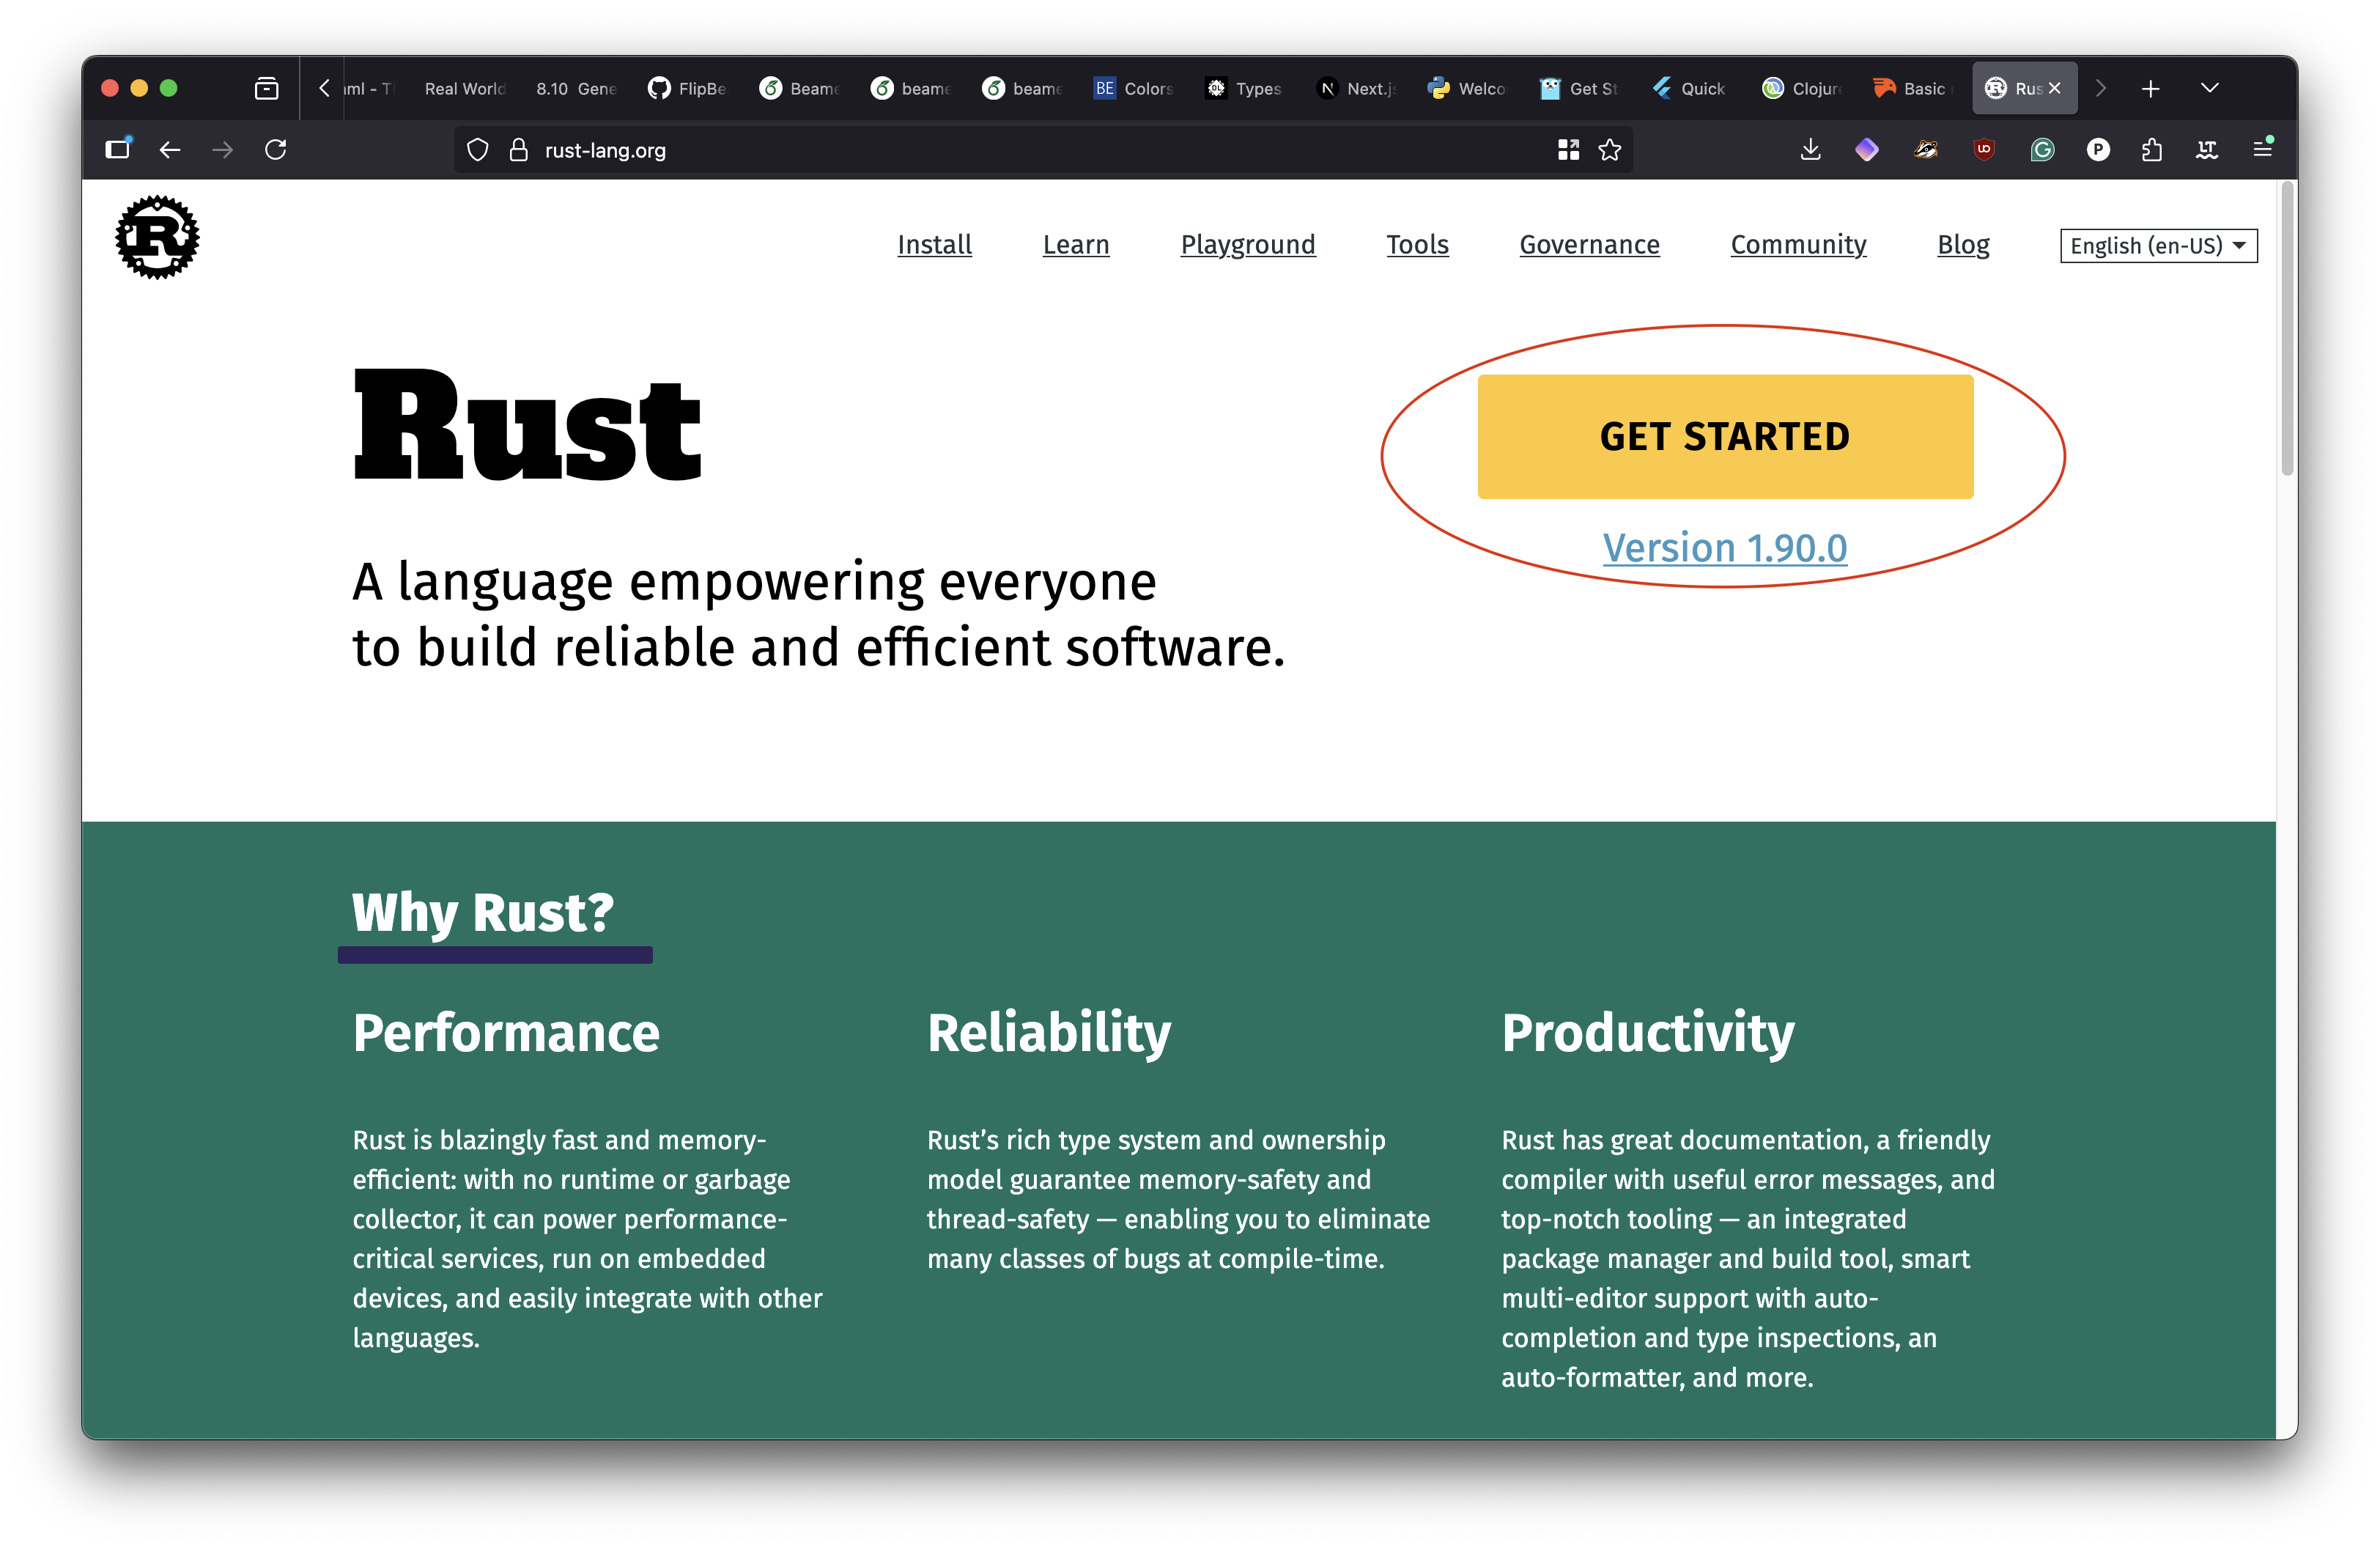
\includegraphics[width=0.45\textwidth]{rust/home.png}
      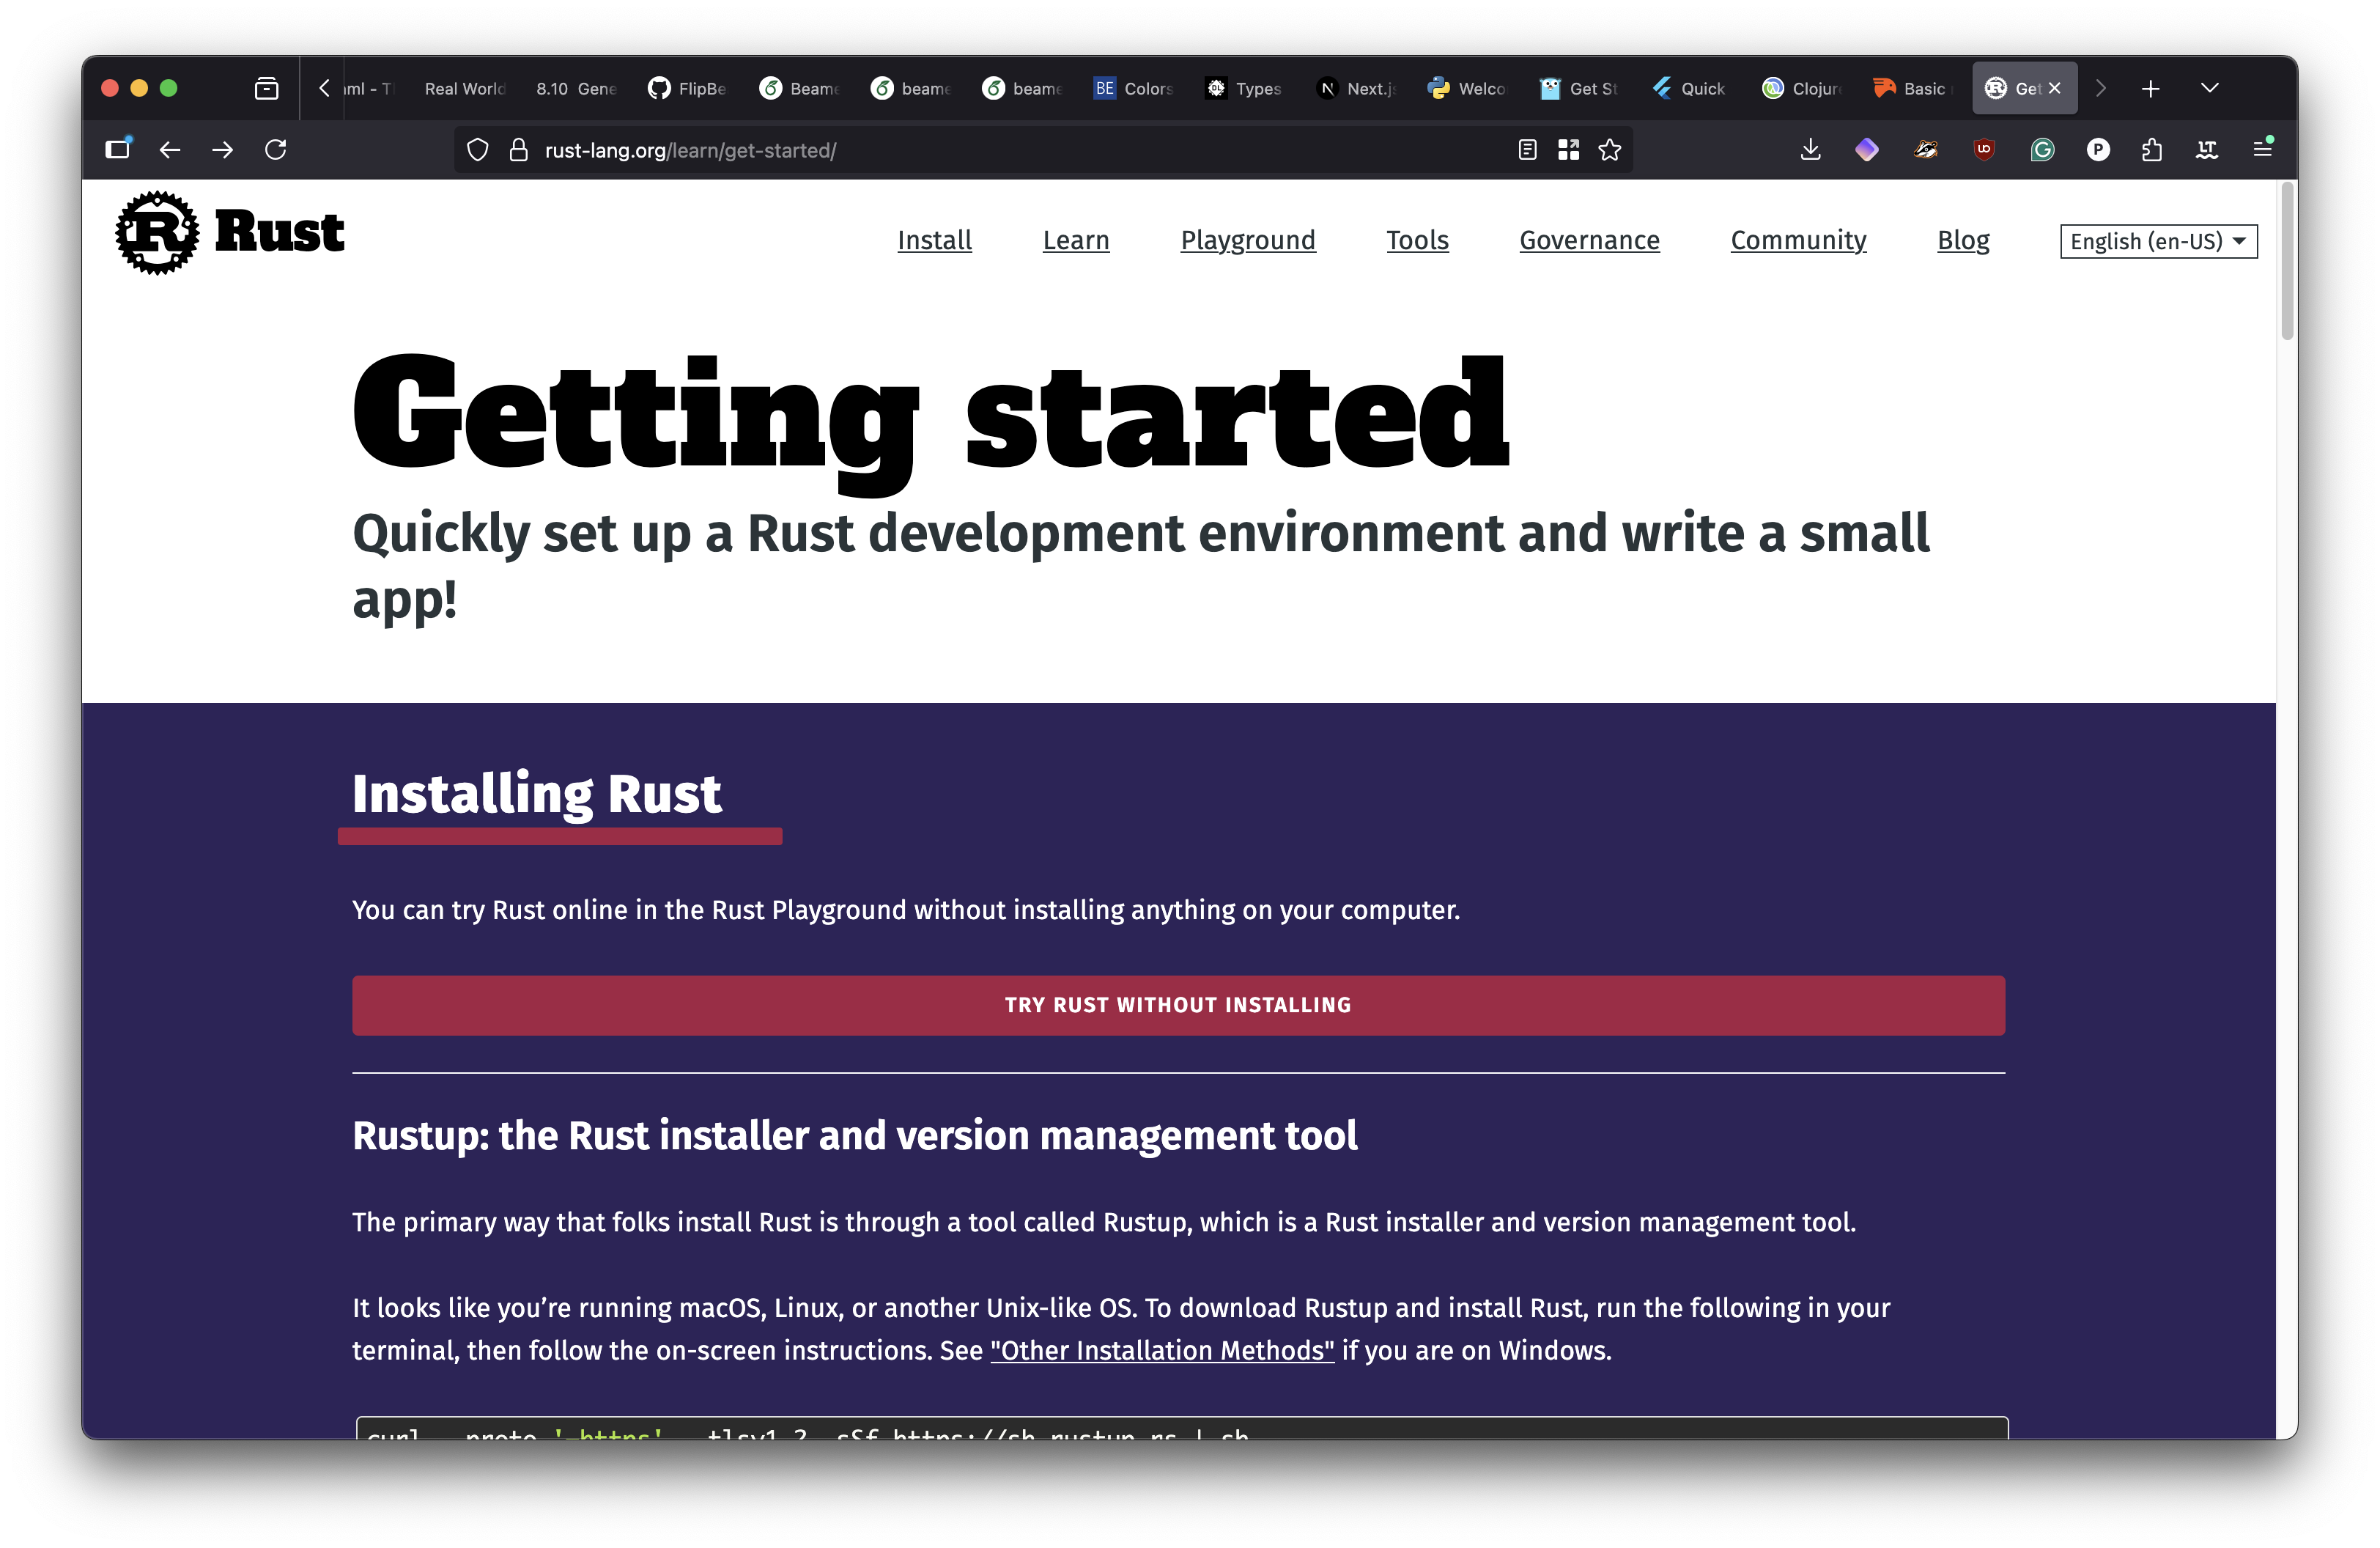
\includegraphics[width=0.45\textwidth]{rust/getstart.png}
   \end{center}
\end{frame}

%-------------------
\begin{frame}{Other examples}
   % Screenshot placeholder:
   % \includegraphics[width=0.7\textwidth]{rocq-old.png}
   \centering
   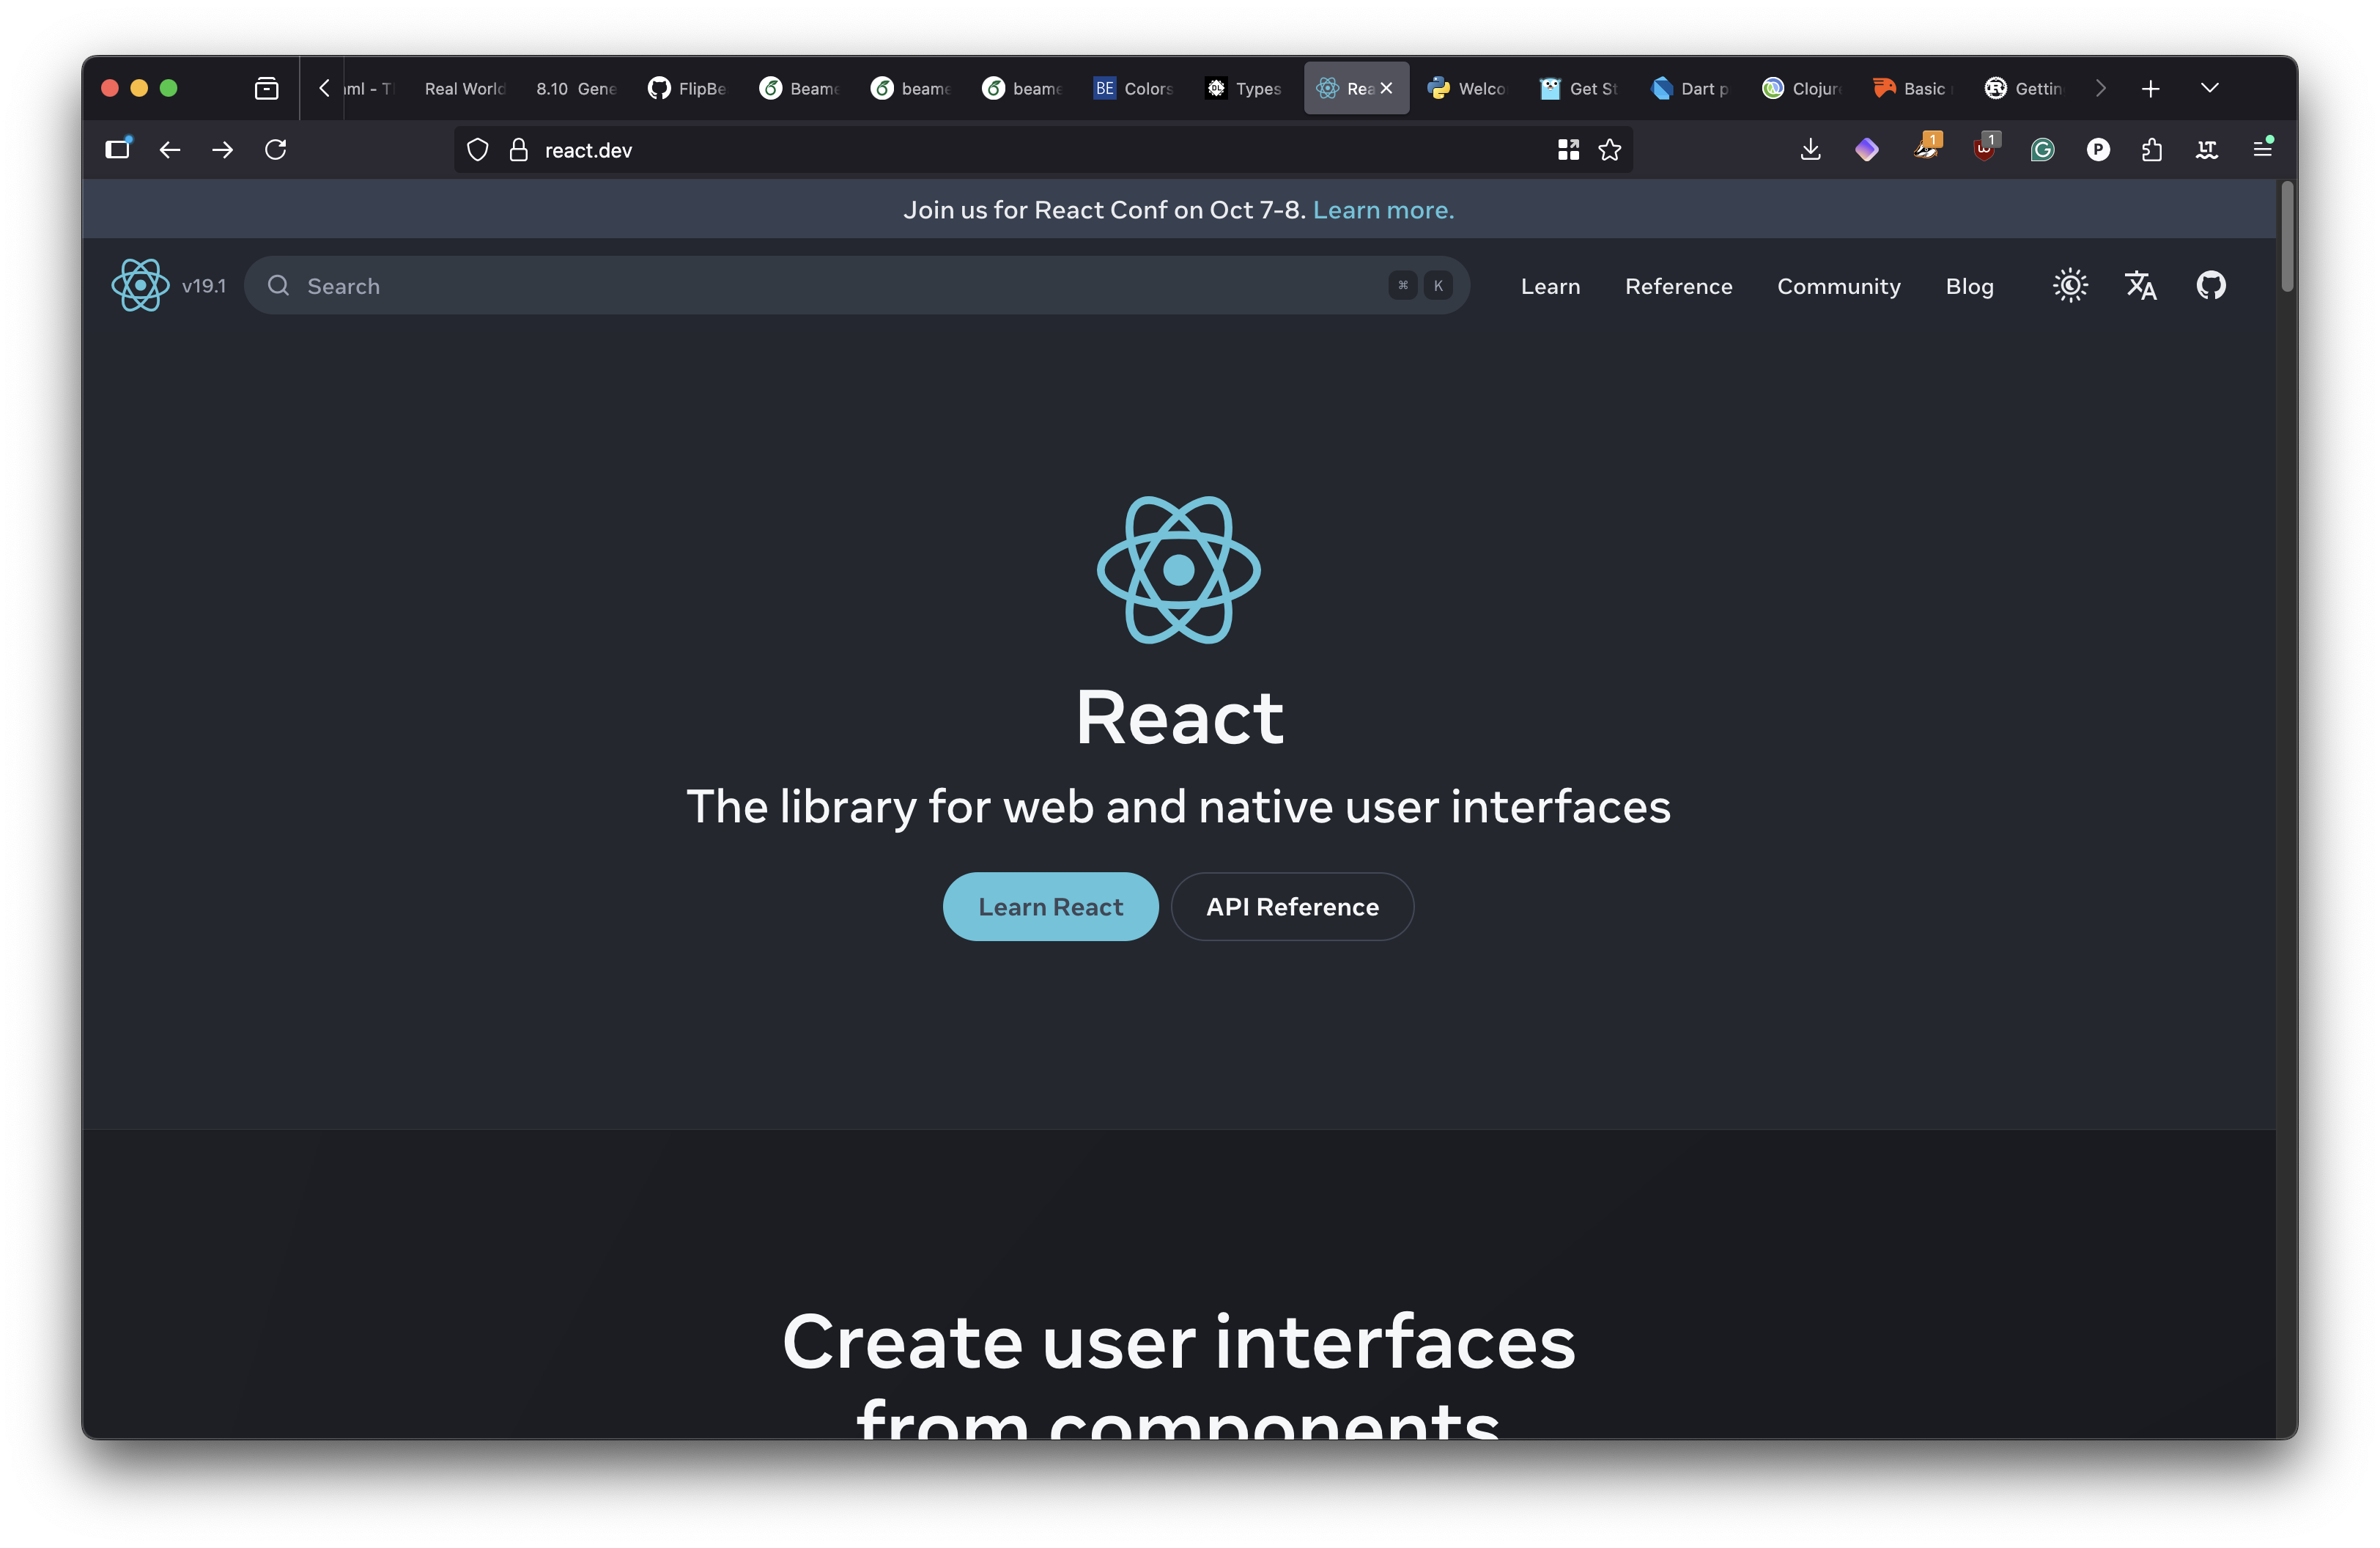
\includegraphics[width=0.45\textwidth]{react/home.png}
   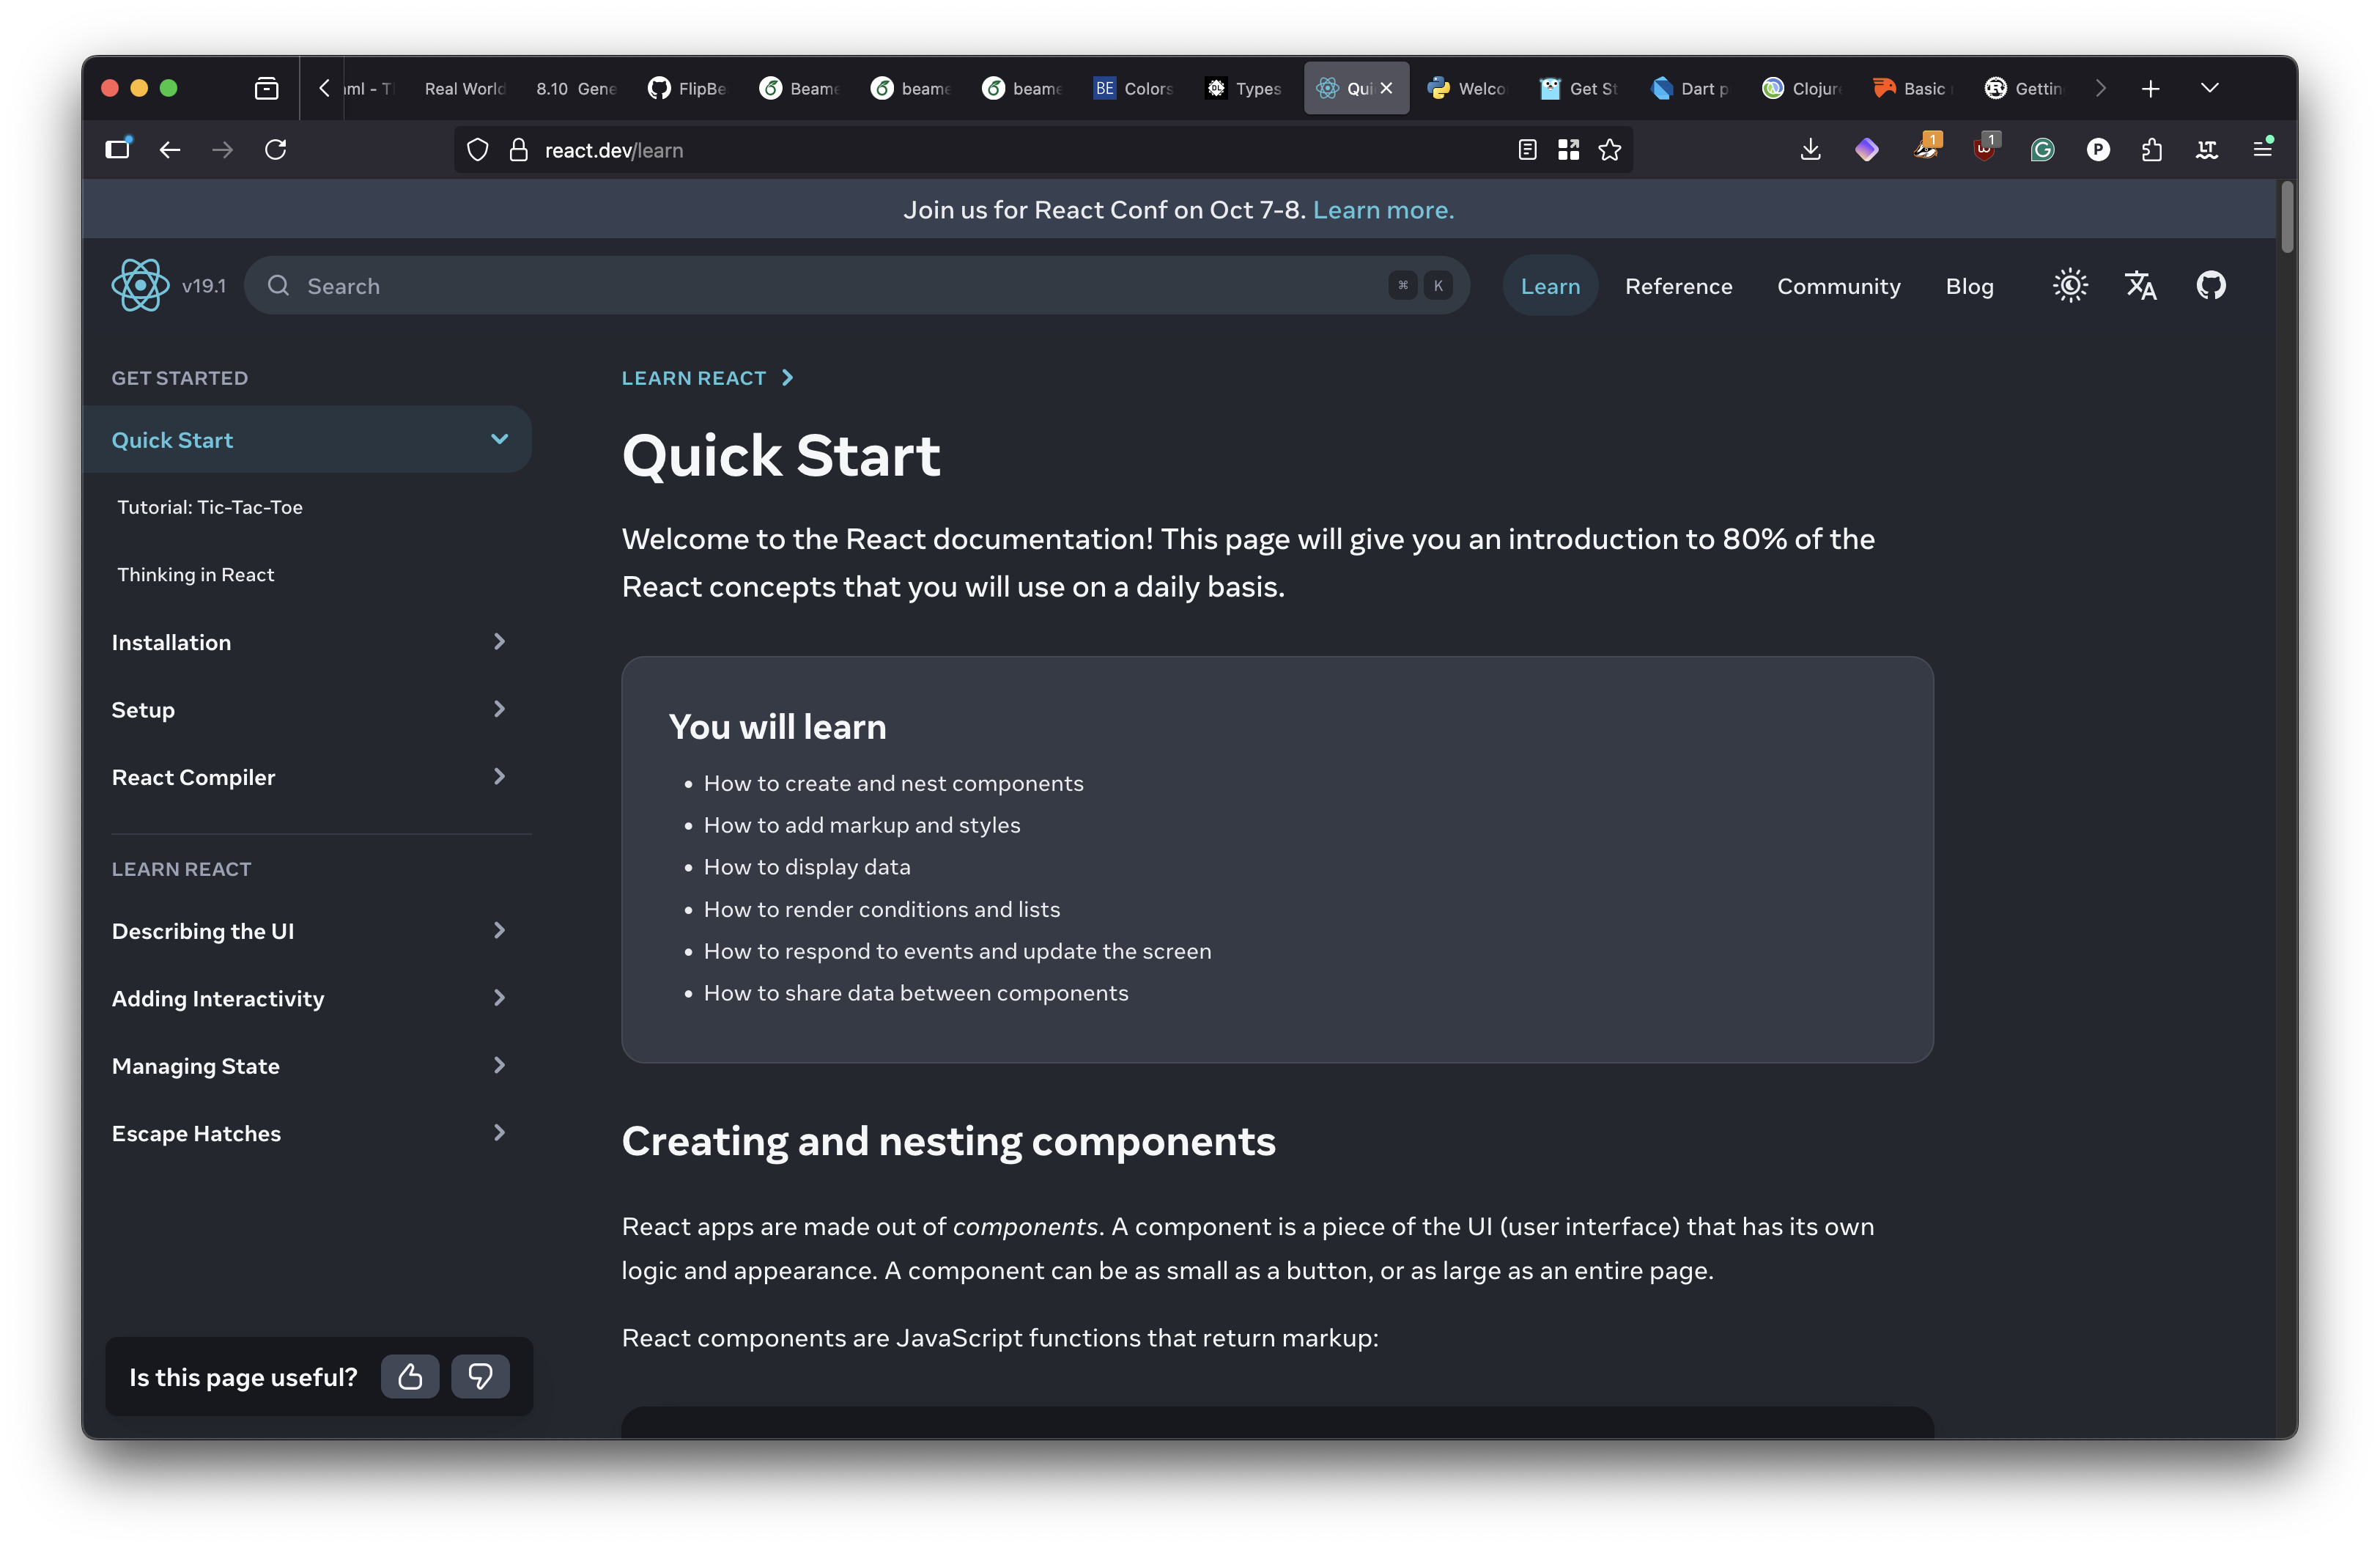
\includegraphics[width=0.45\textwidth]{react/learn.png}


   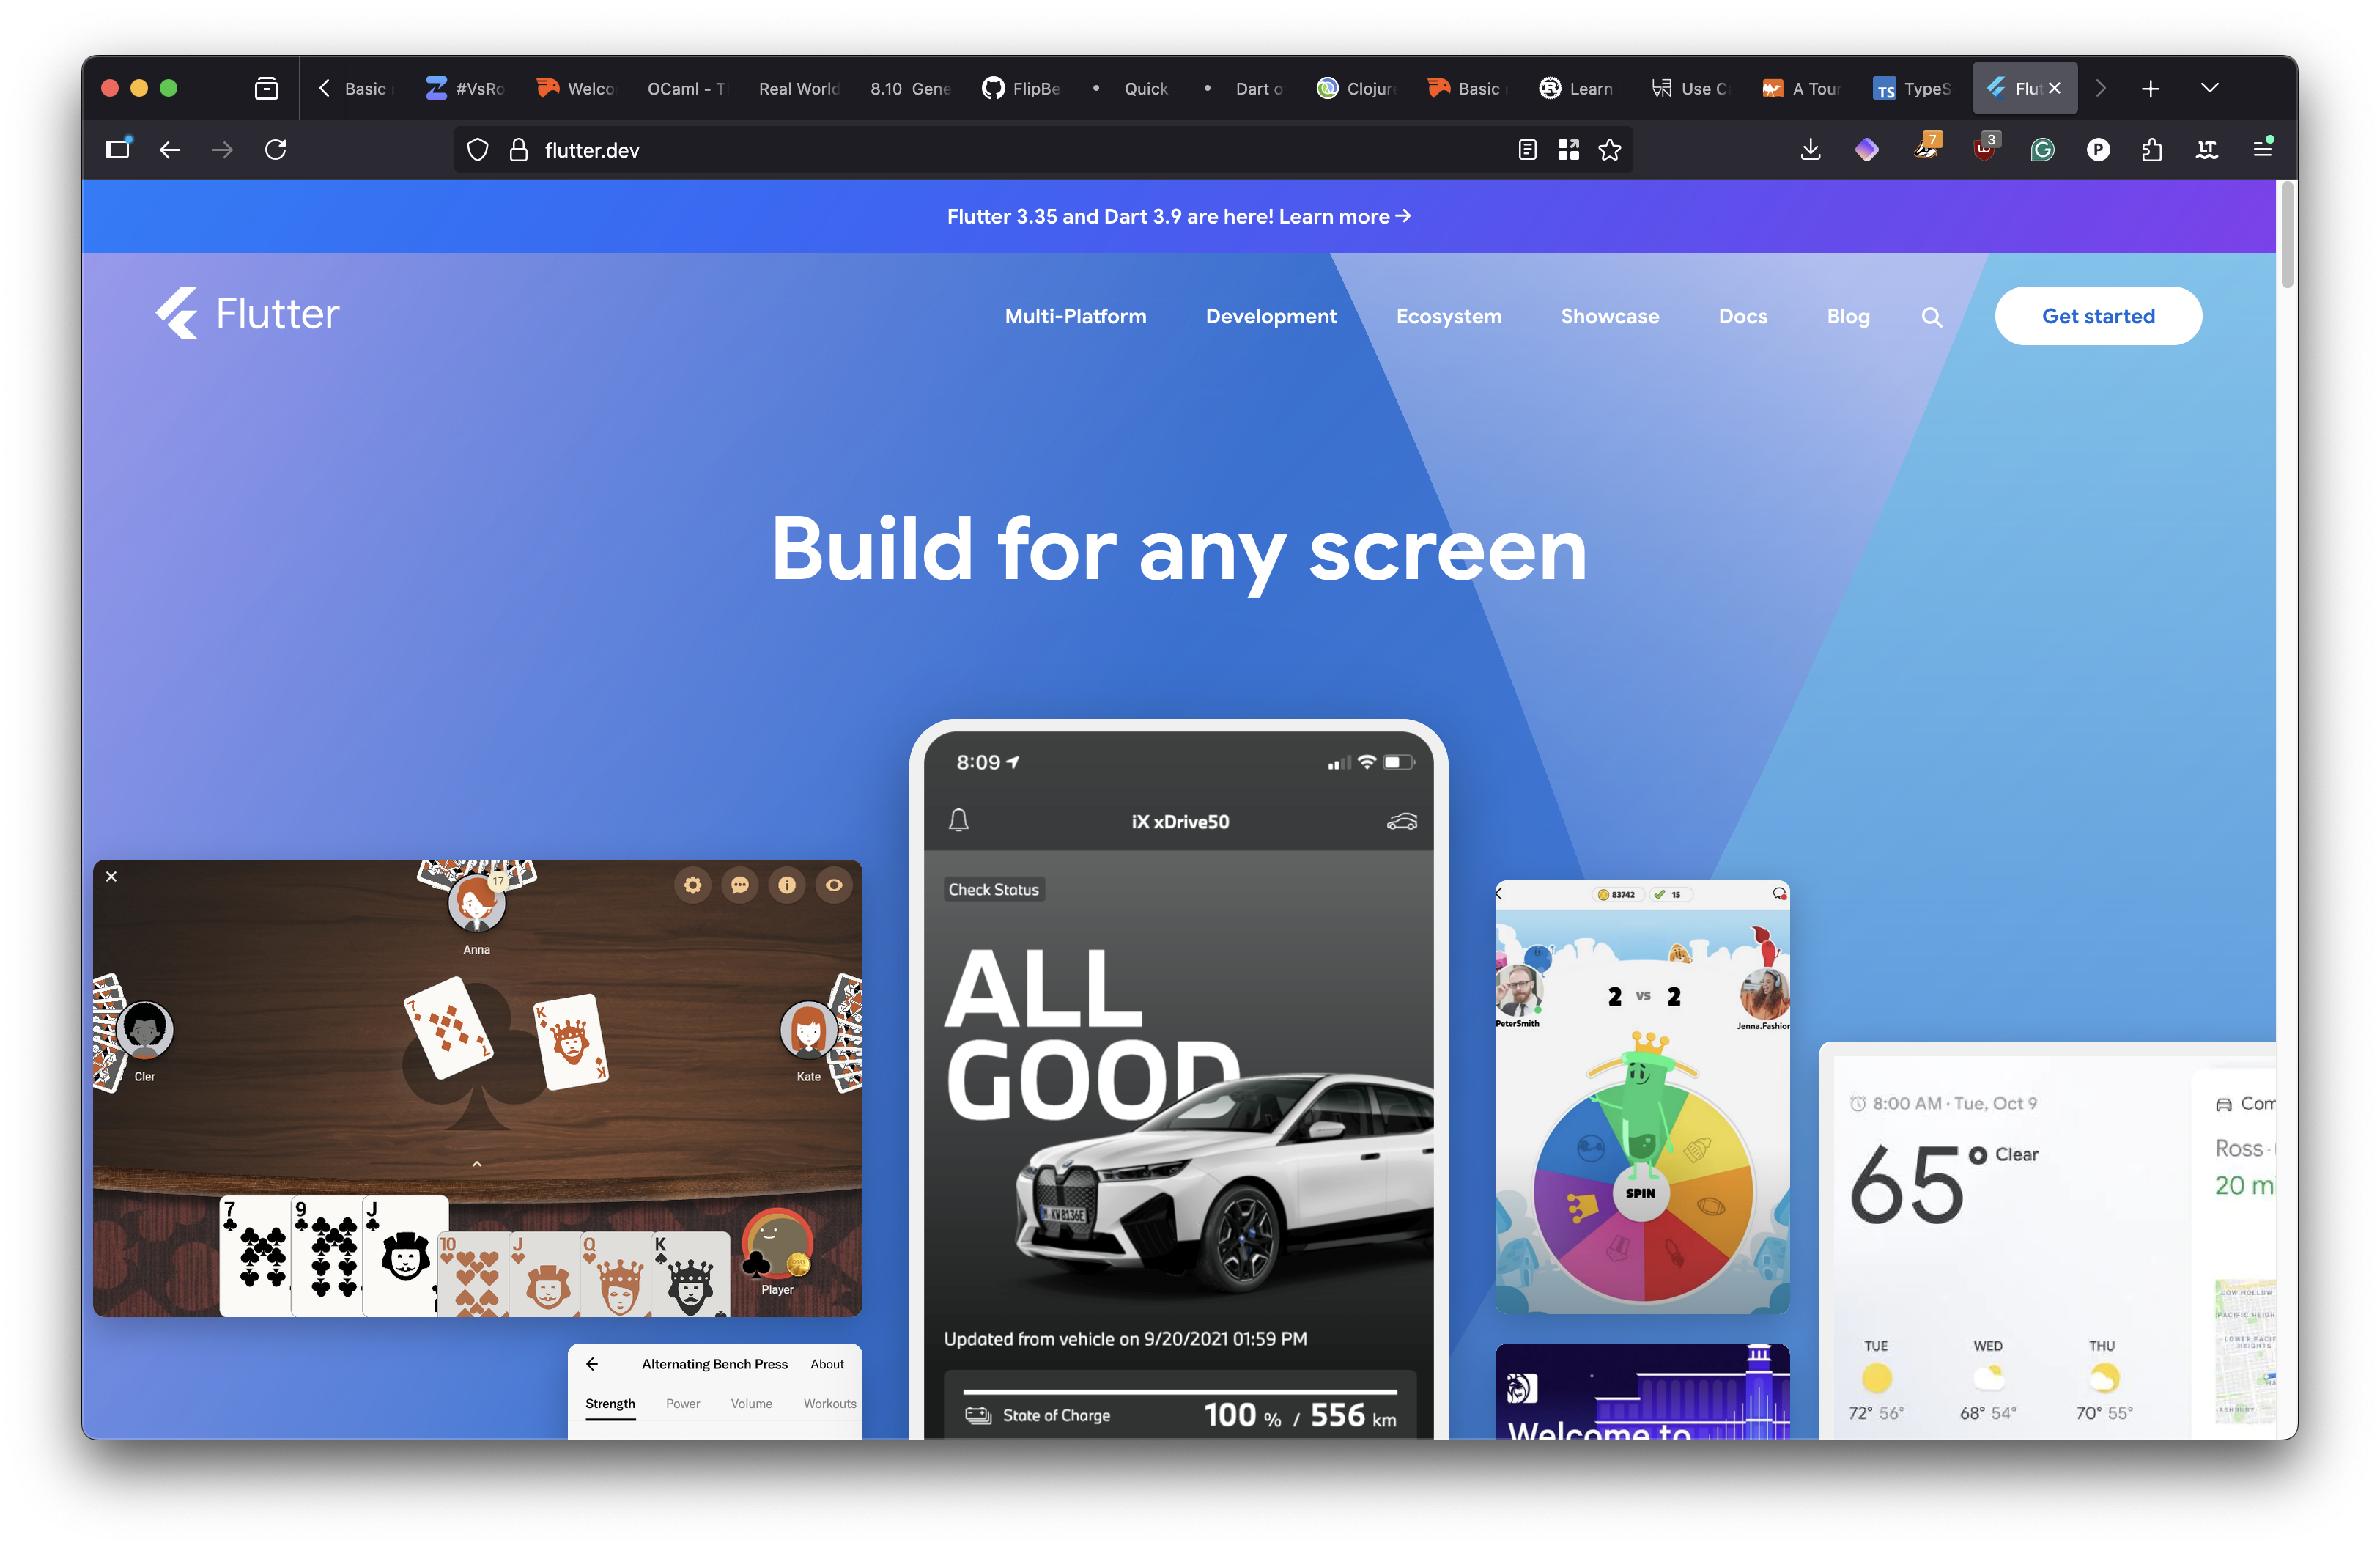
\includegraphics[width=0.45\textwidth]{flutter/home.png}
   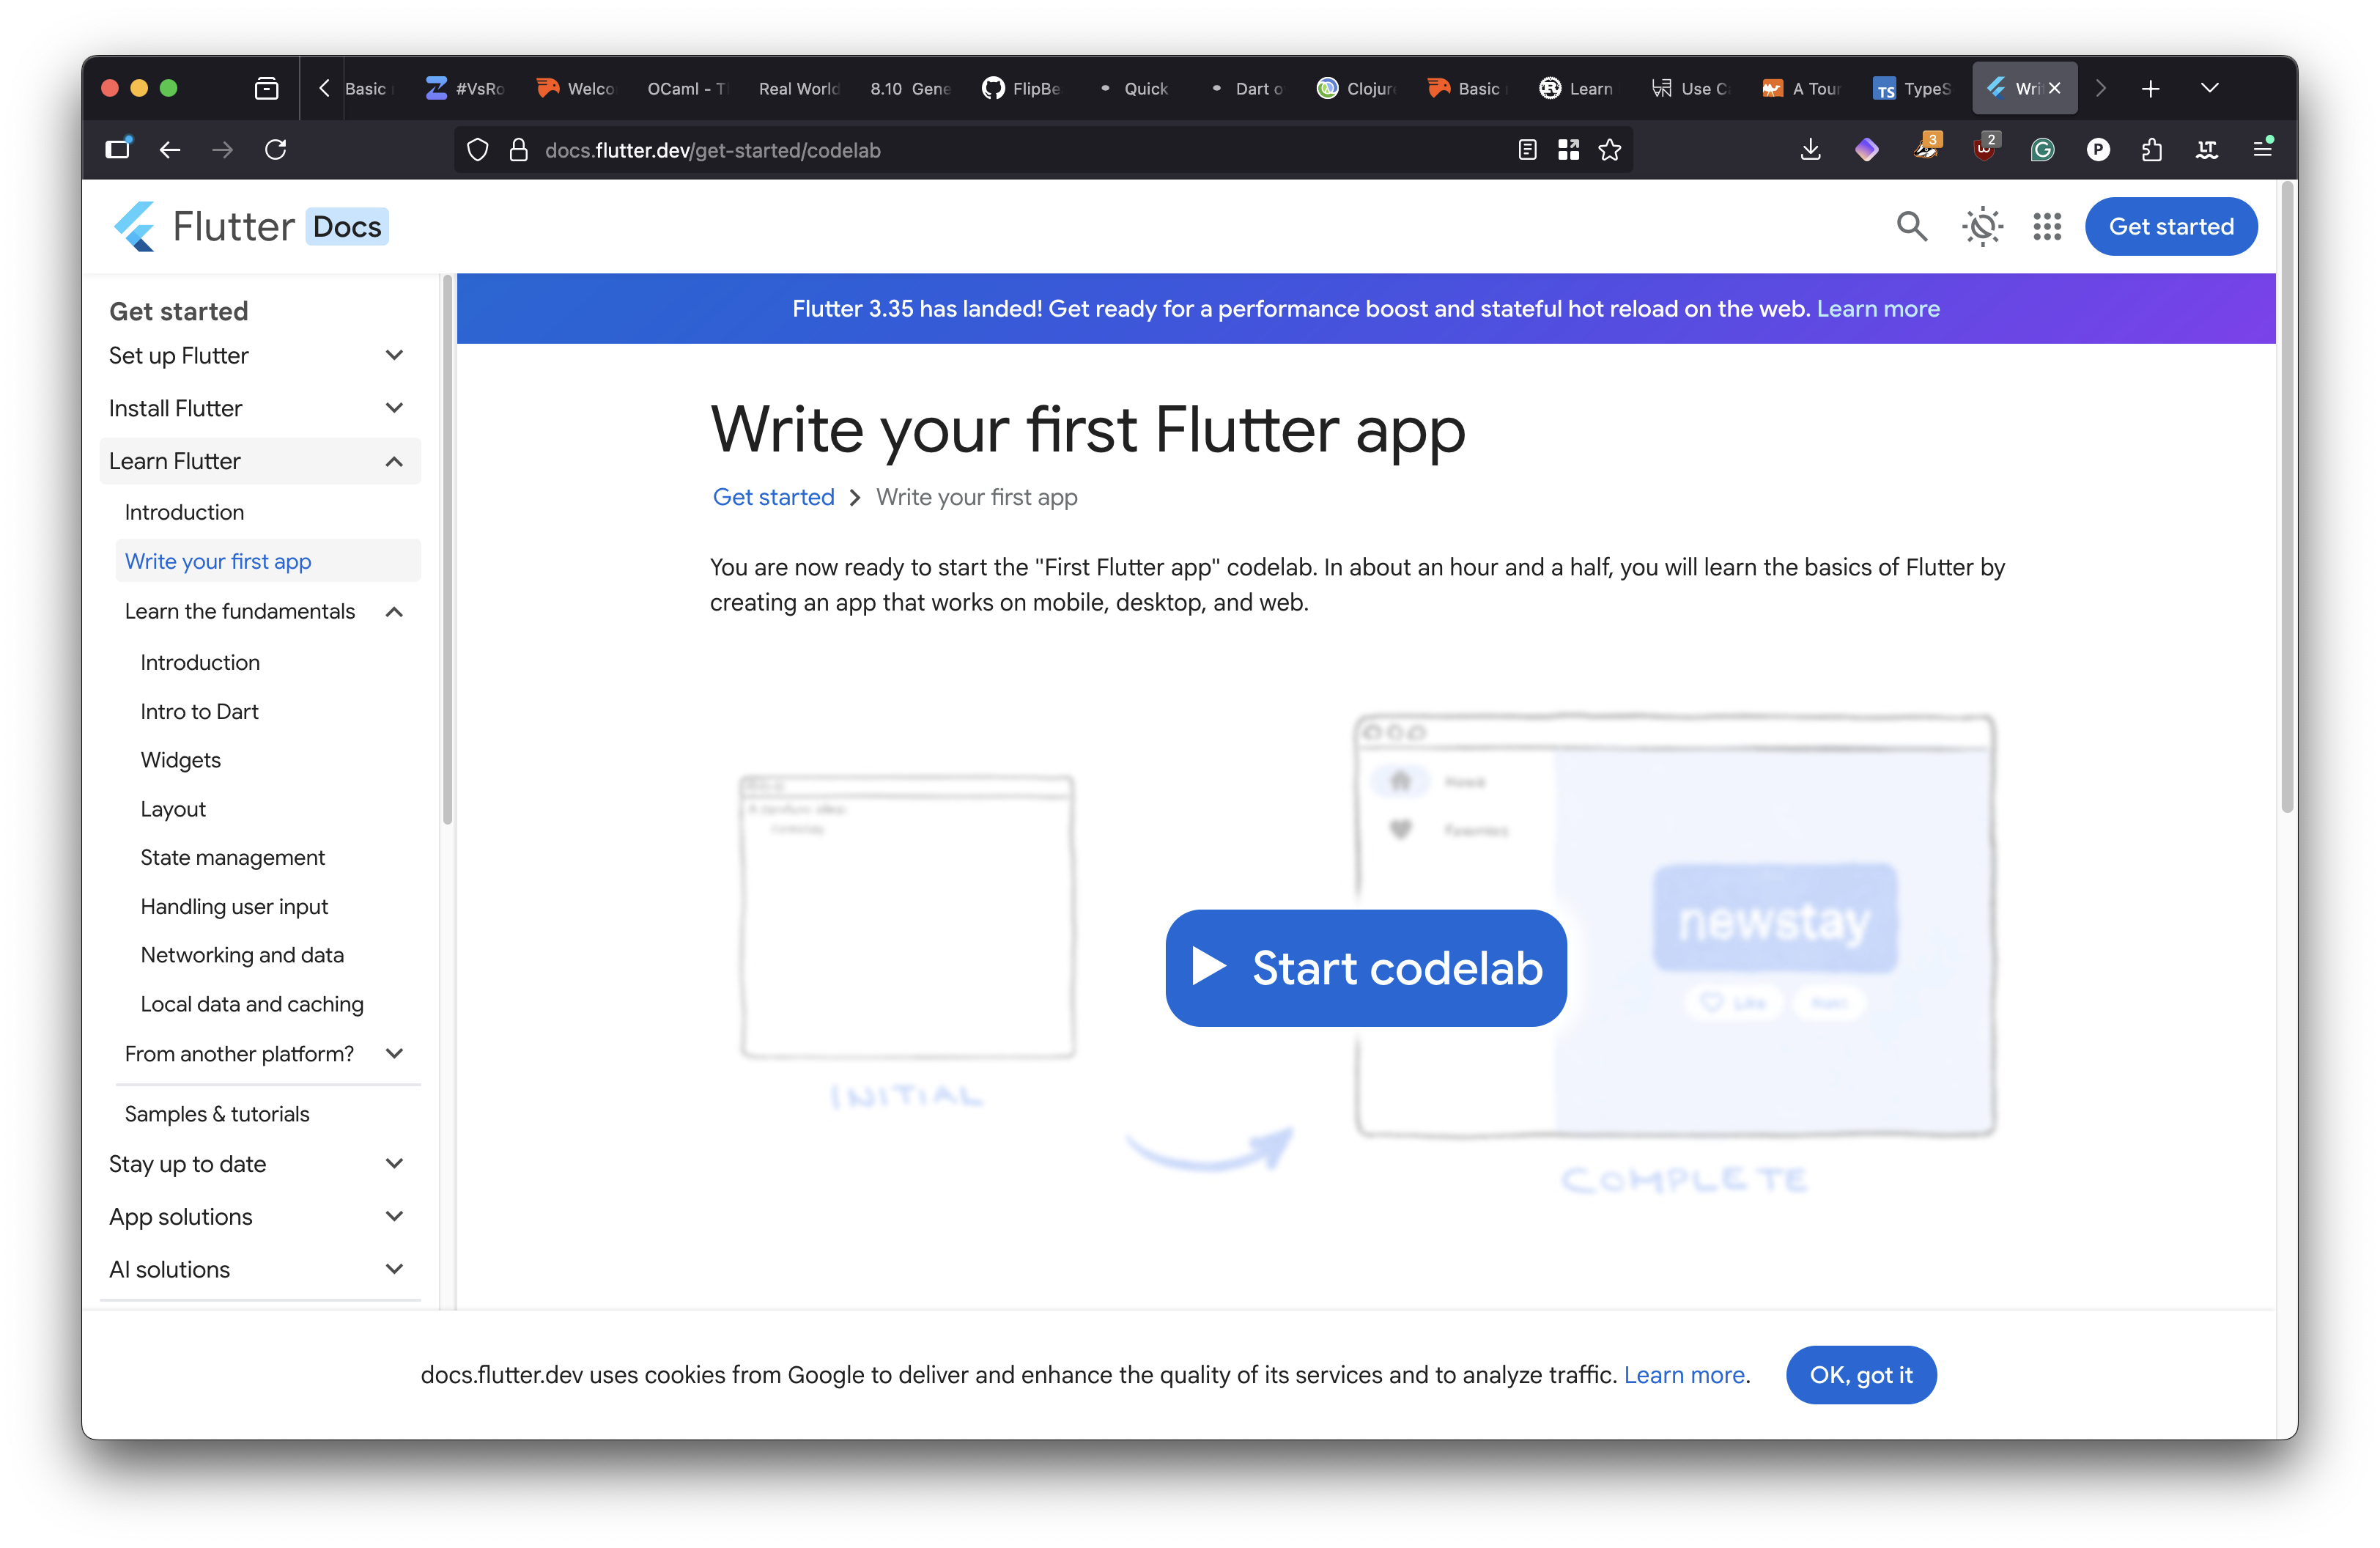
\includegraphics[width=0.45\textwidth]{flutter/learn.png}
\end{frame}

%-------------------
\begin{frame}{What I found for Coq}
   \centering
   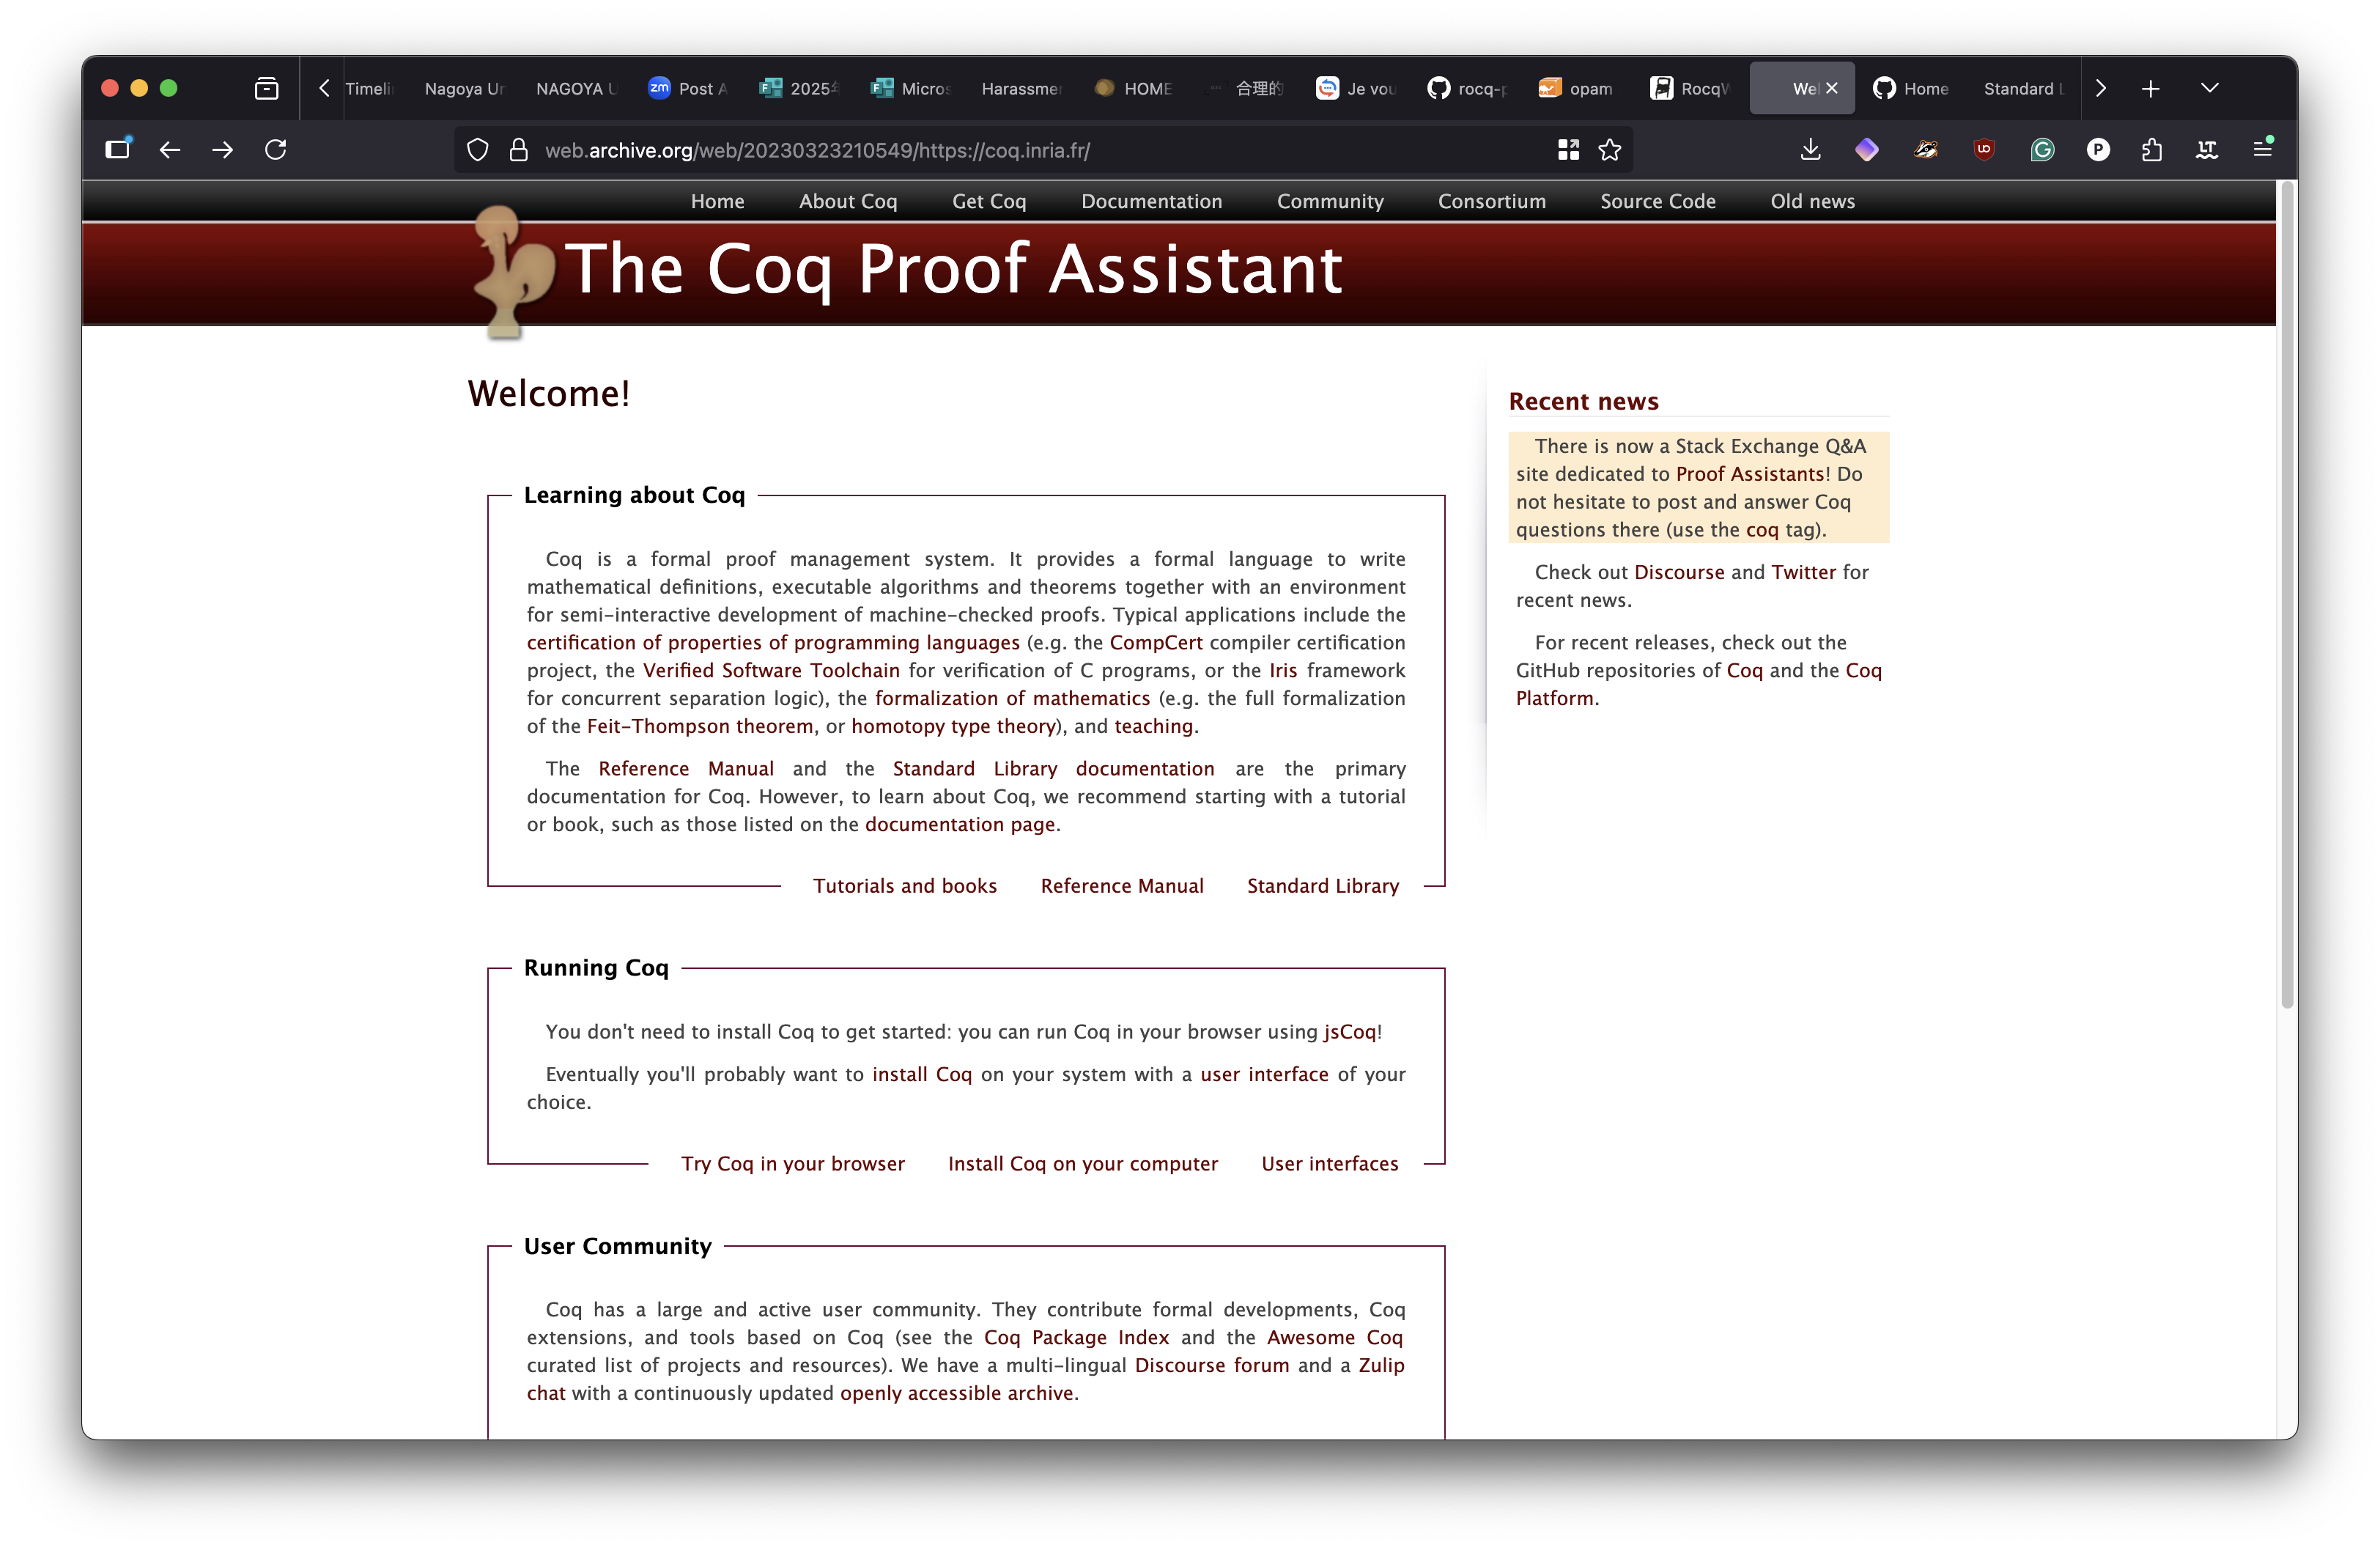
\includegraphics[width=0.45\textwidth]{coq/home.png}
   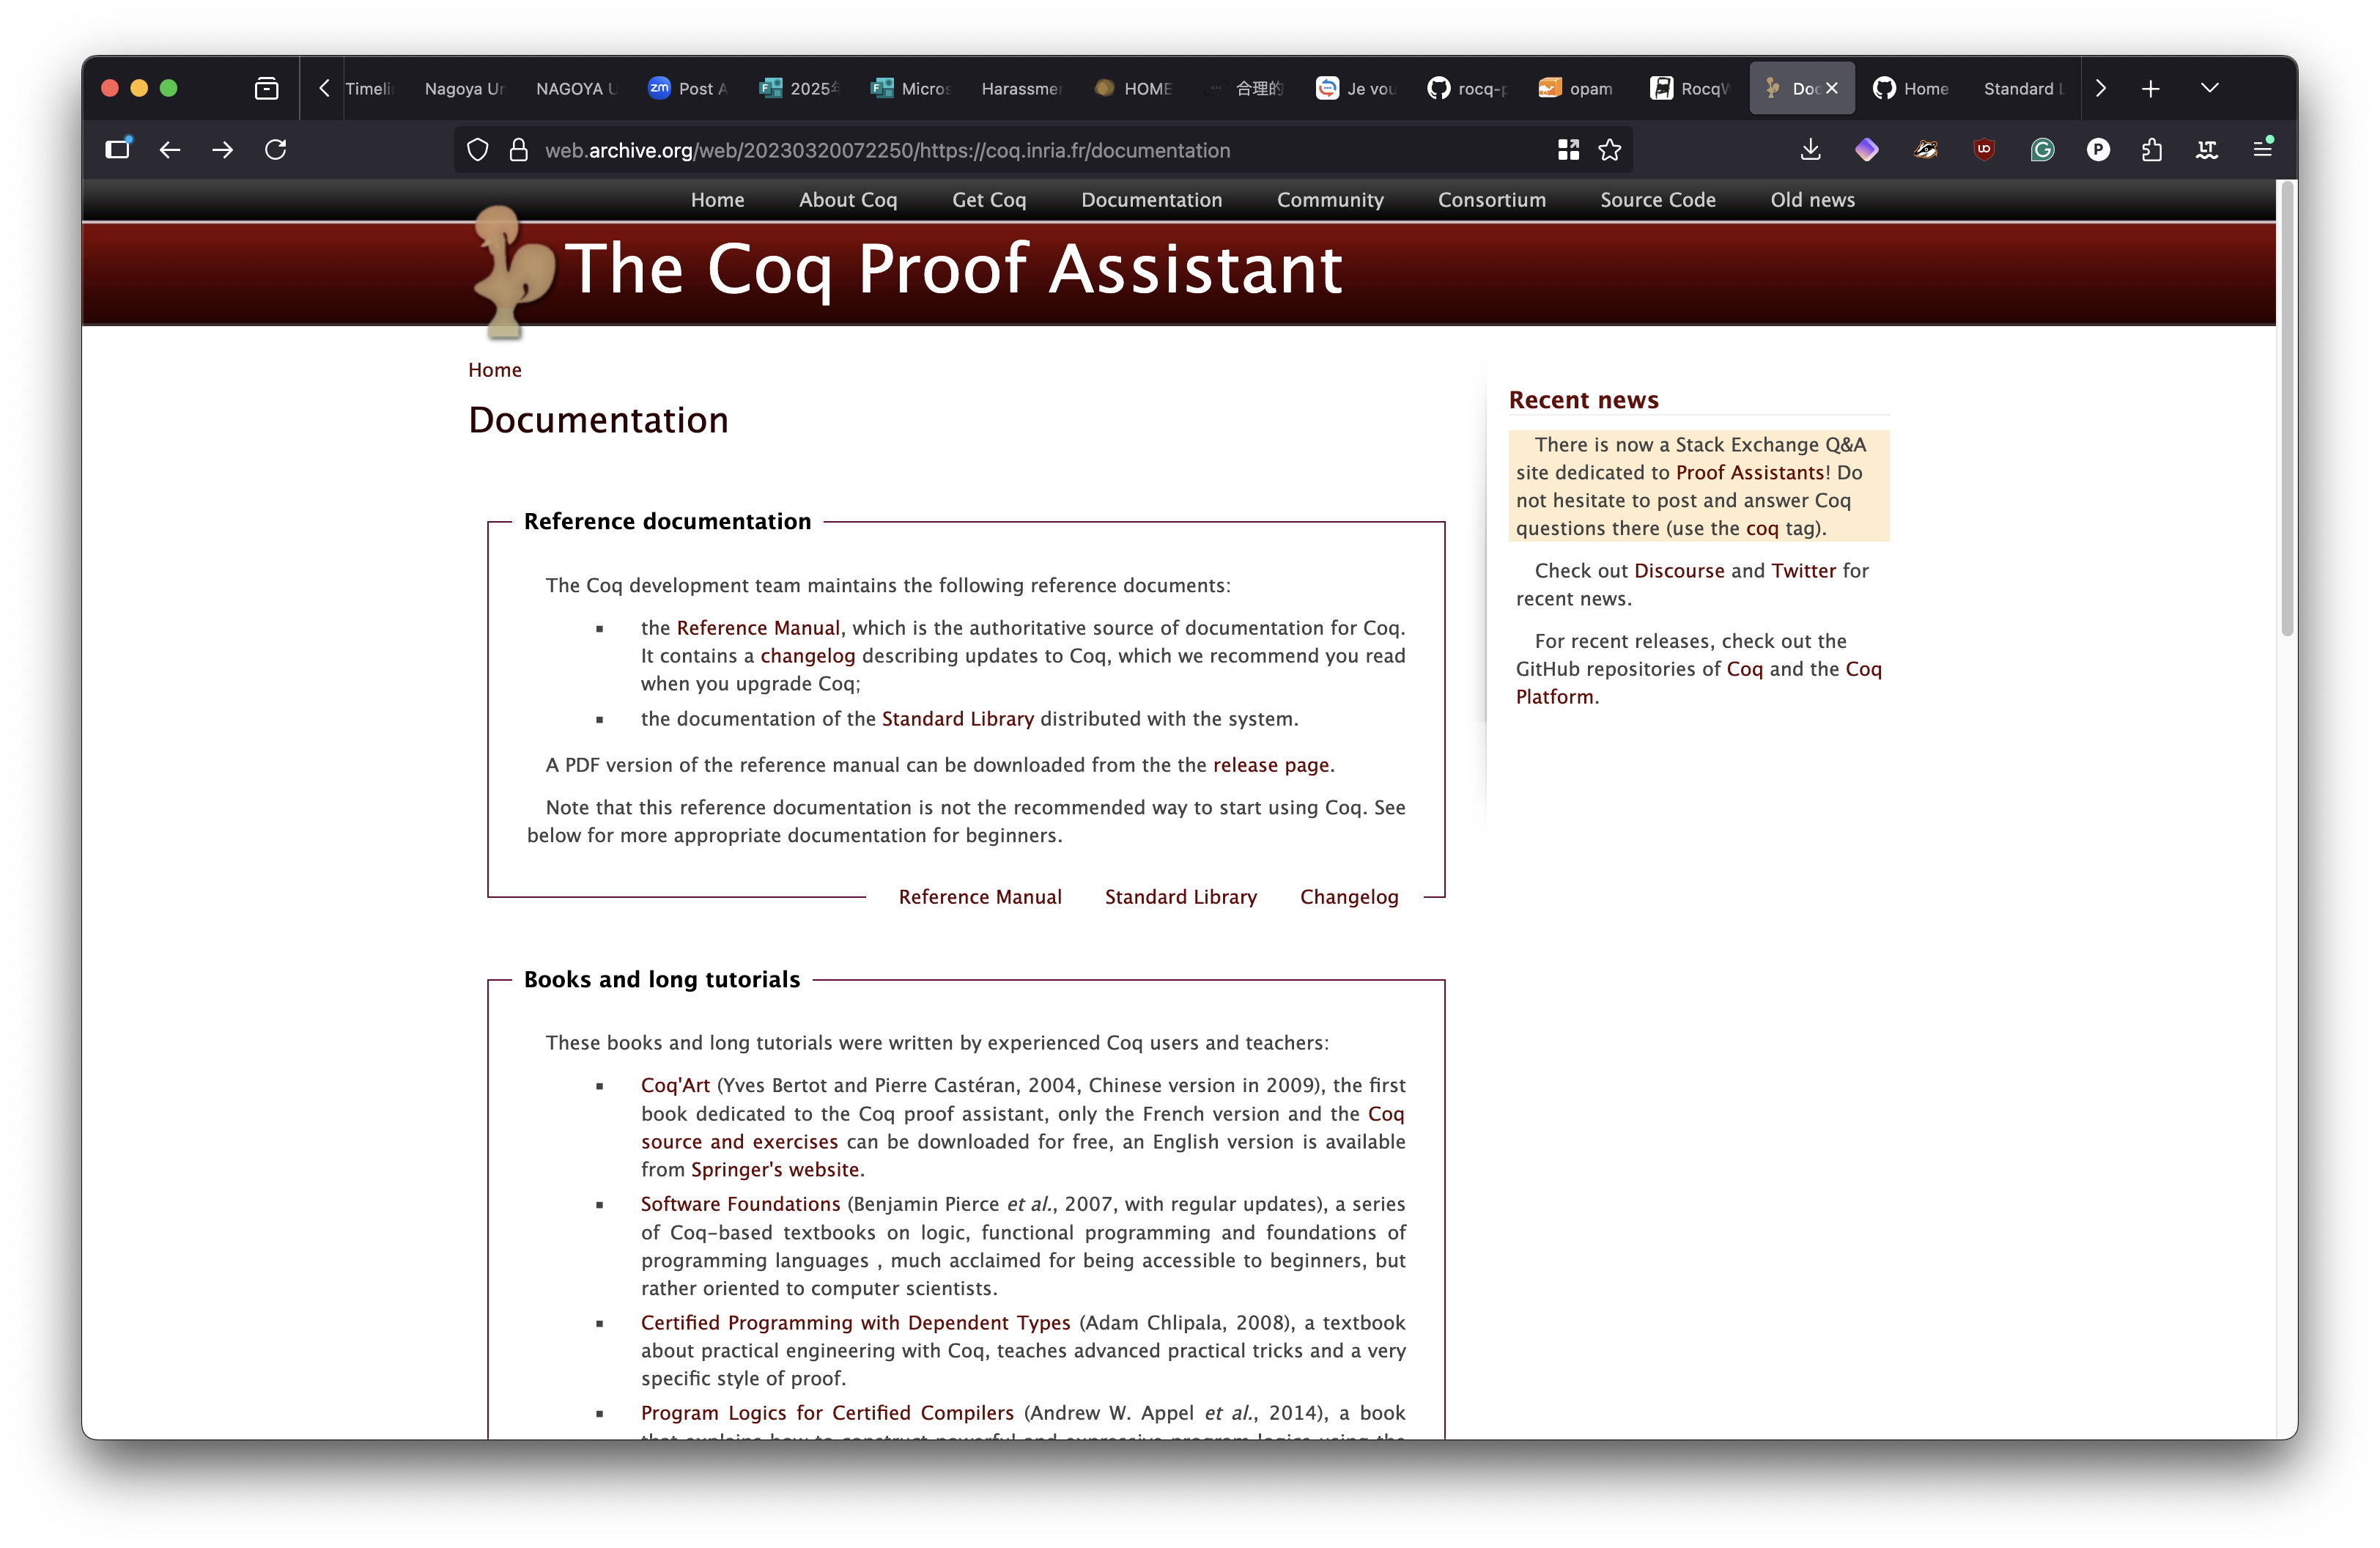
\includegraphics[width=0.45\textwidth]{coq/documentation.png}


   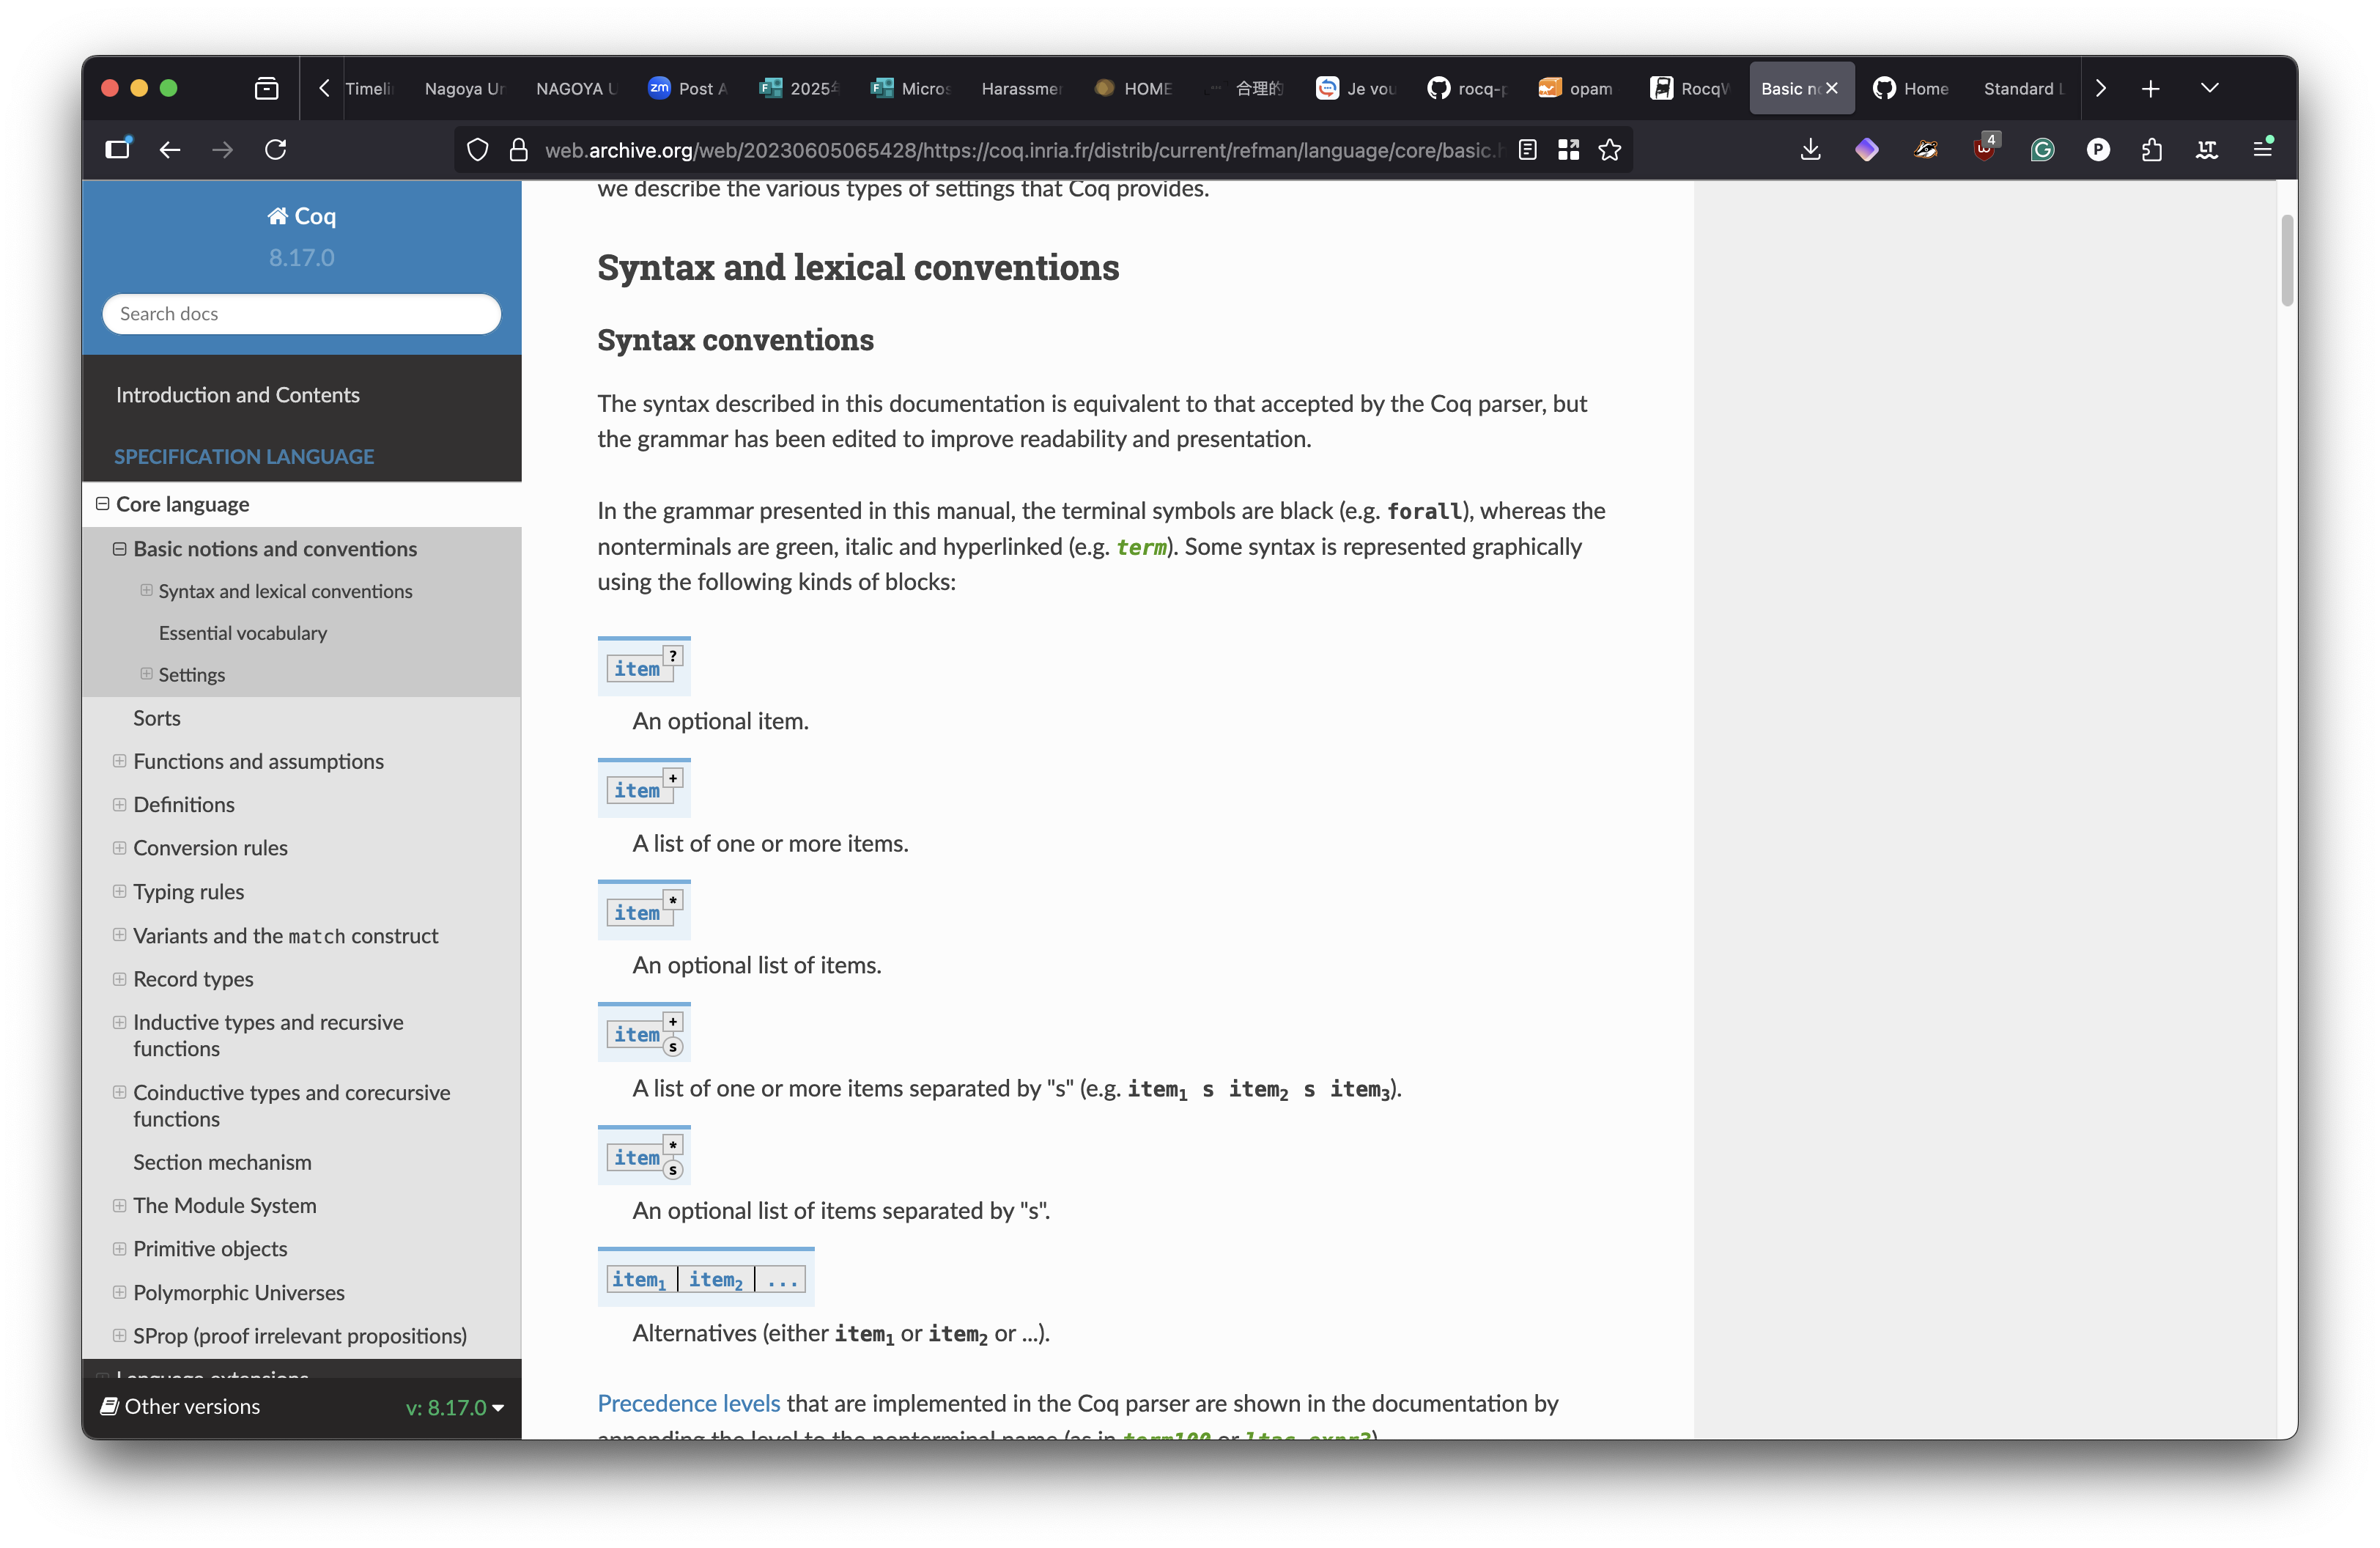
\includegraphics[width=0.45\textwidth]{coq/manual1.png}
   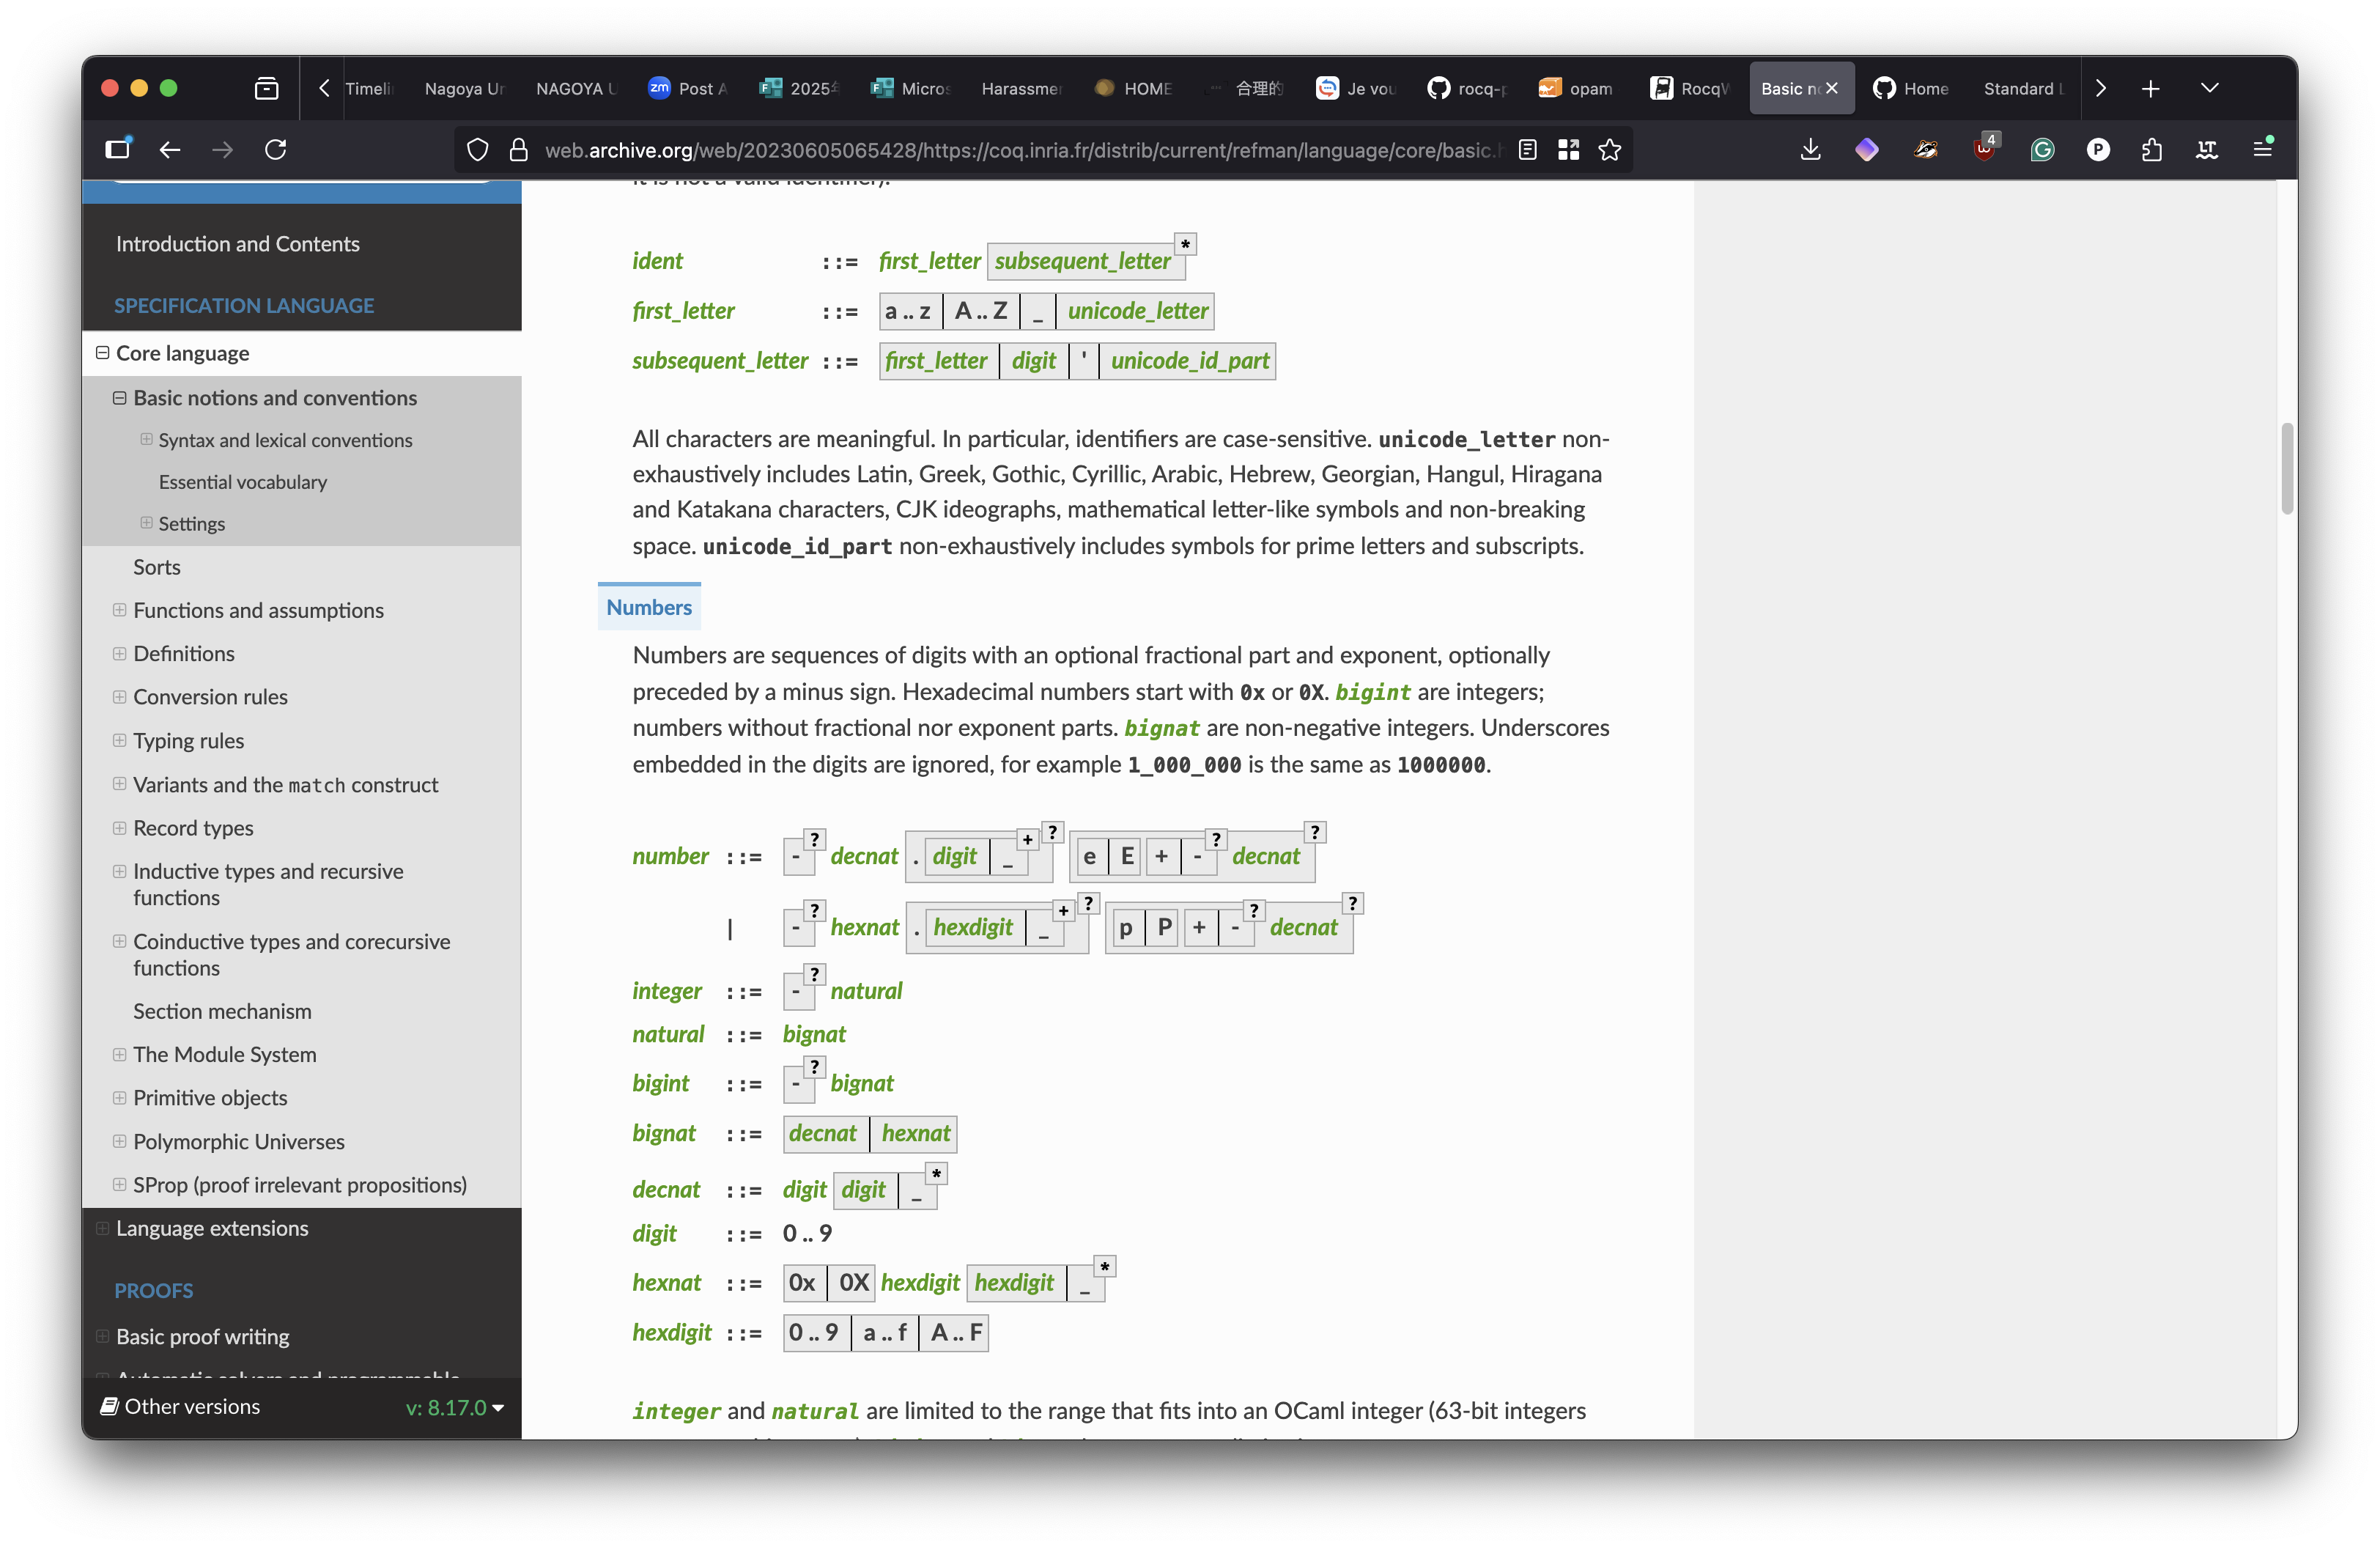
\includegraphics[width=0.45\textwidth]{coq/manual2.png}
\end{frame}

%-------------------
\begin{frame}{Rocq is better but...}
   \centering
   
\includegraphics[width=0.45\textwidth]{rocq/home.png}
   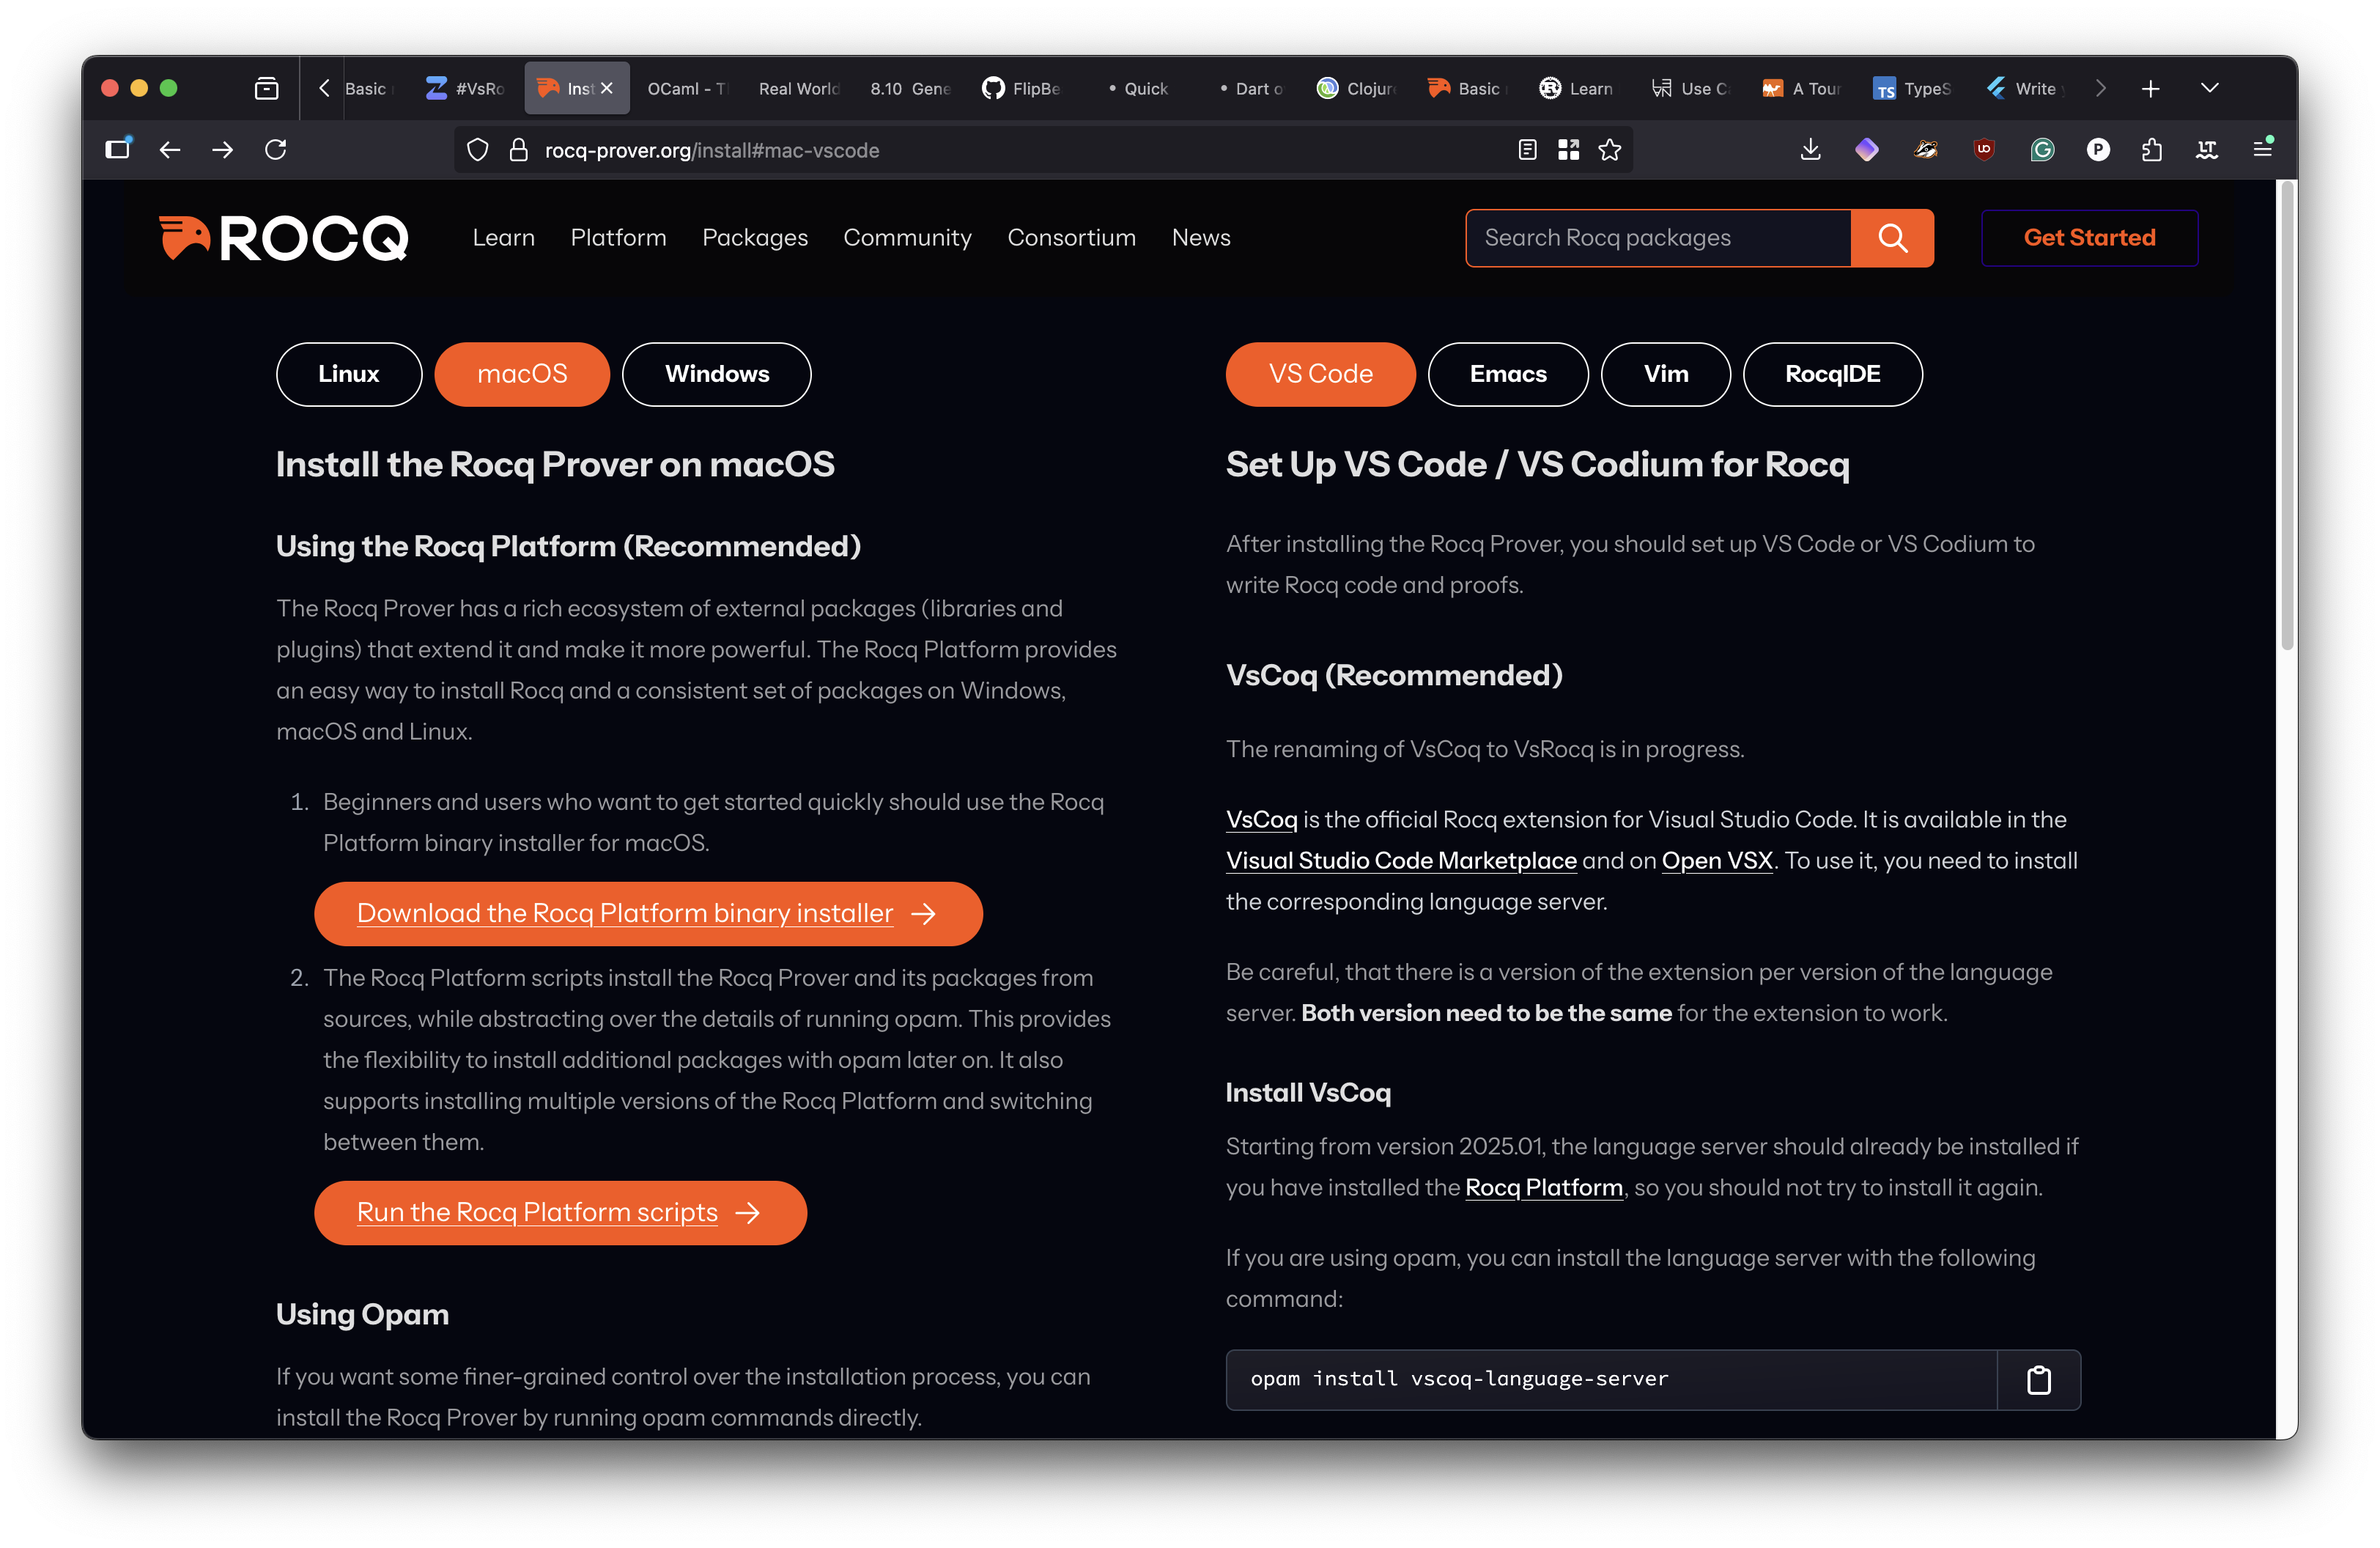
\includegraphics[width=0.45\textwidth]{rocq/install.png}

   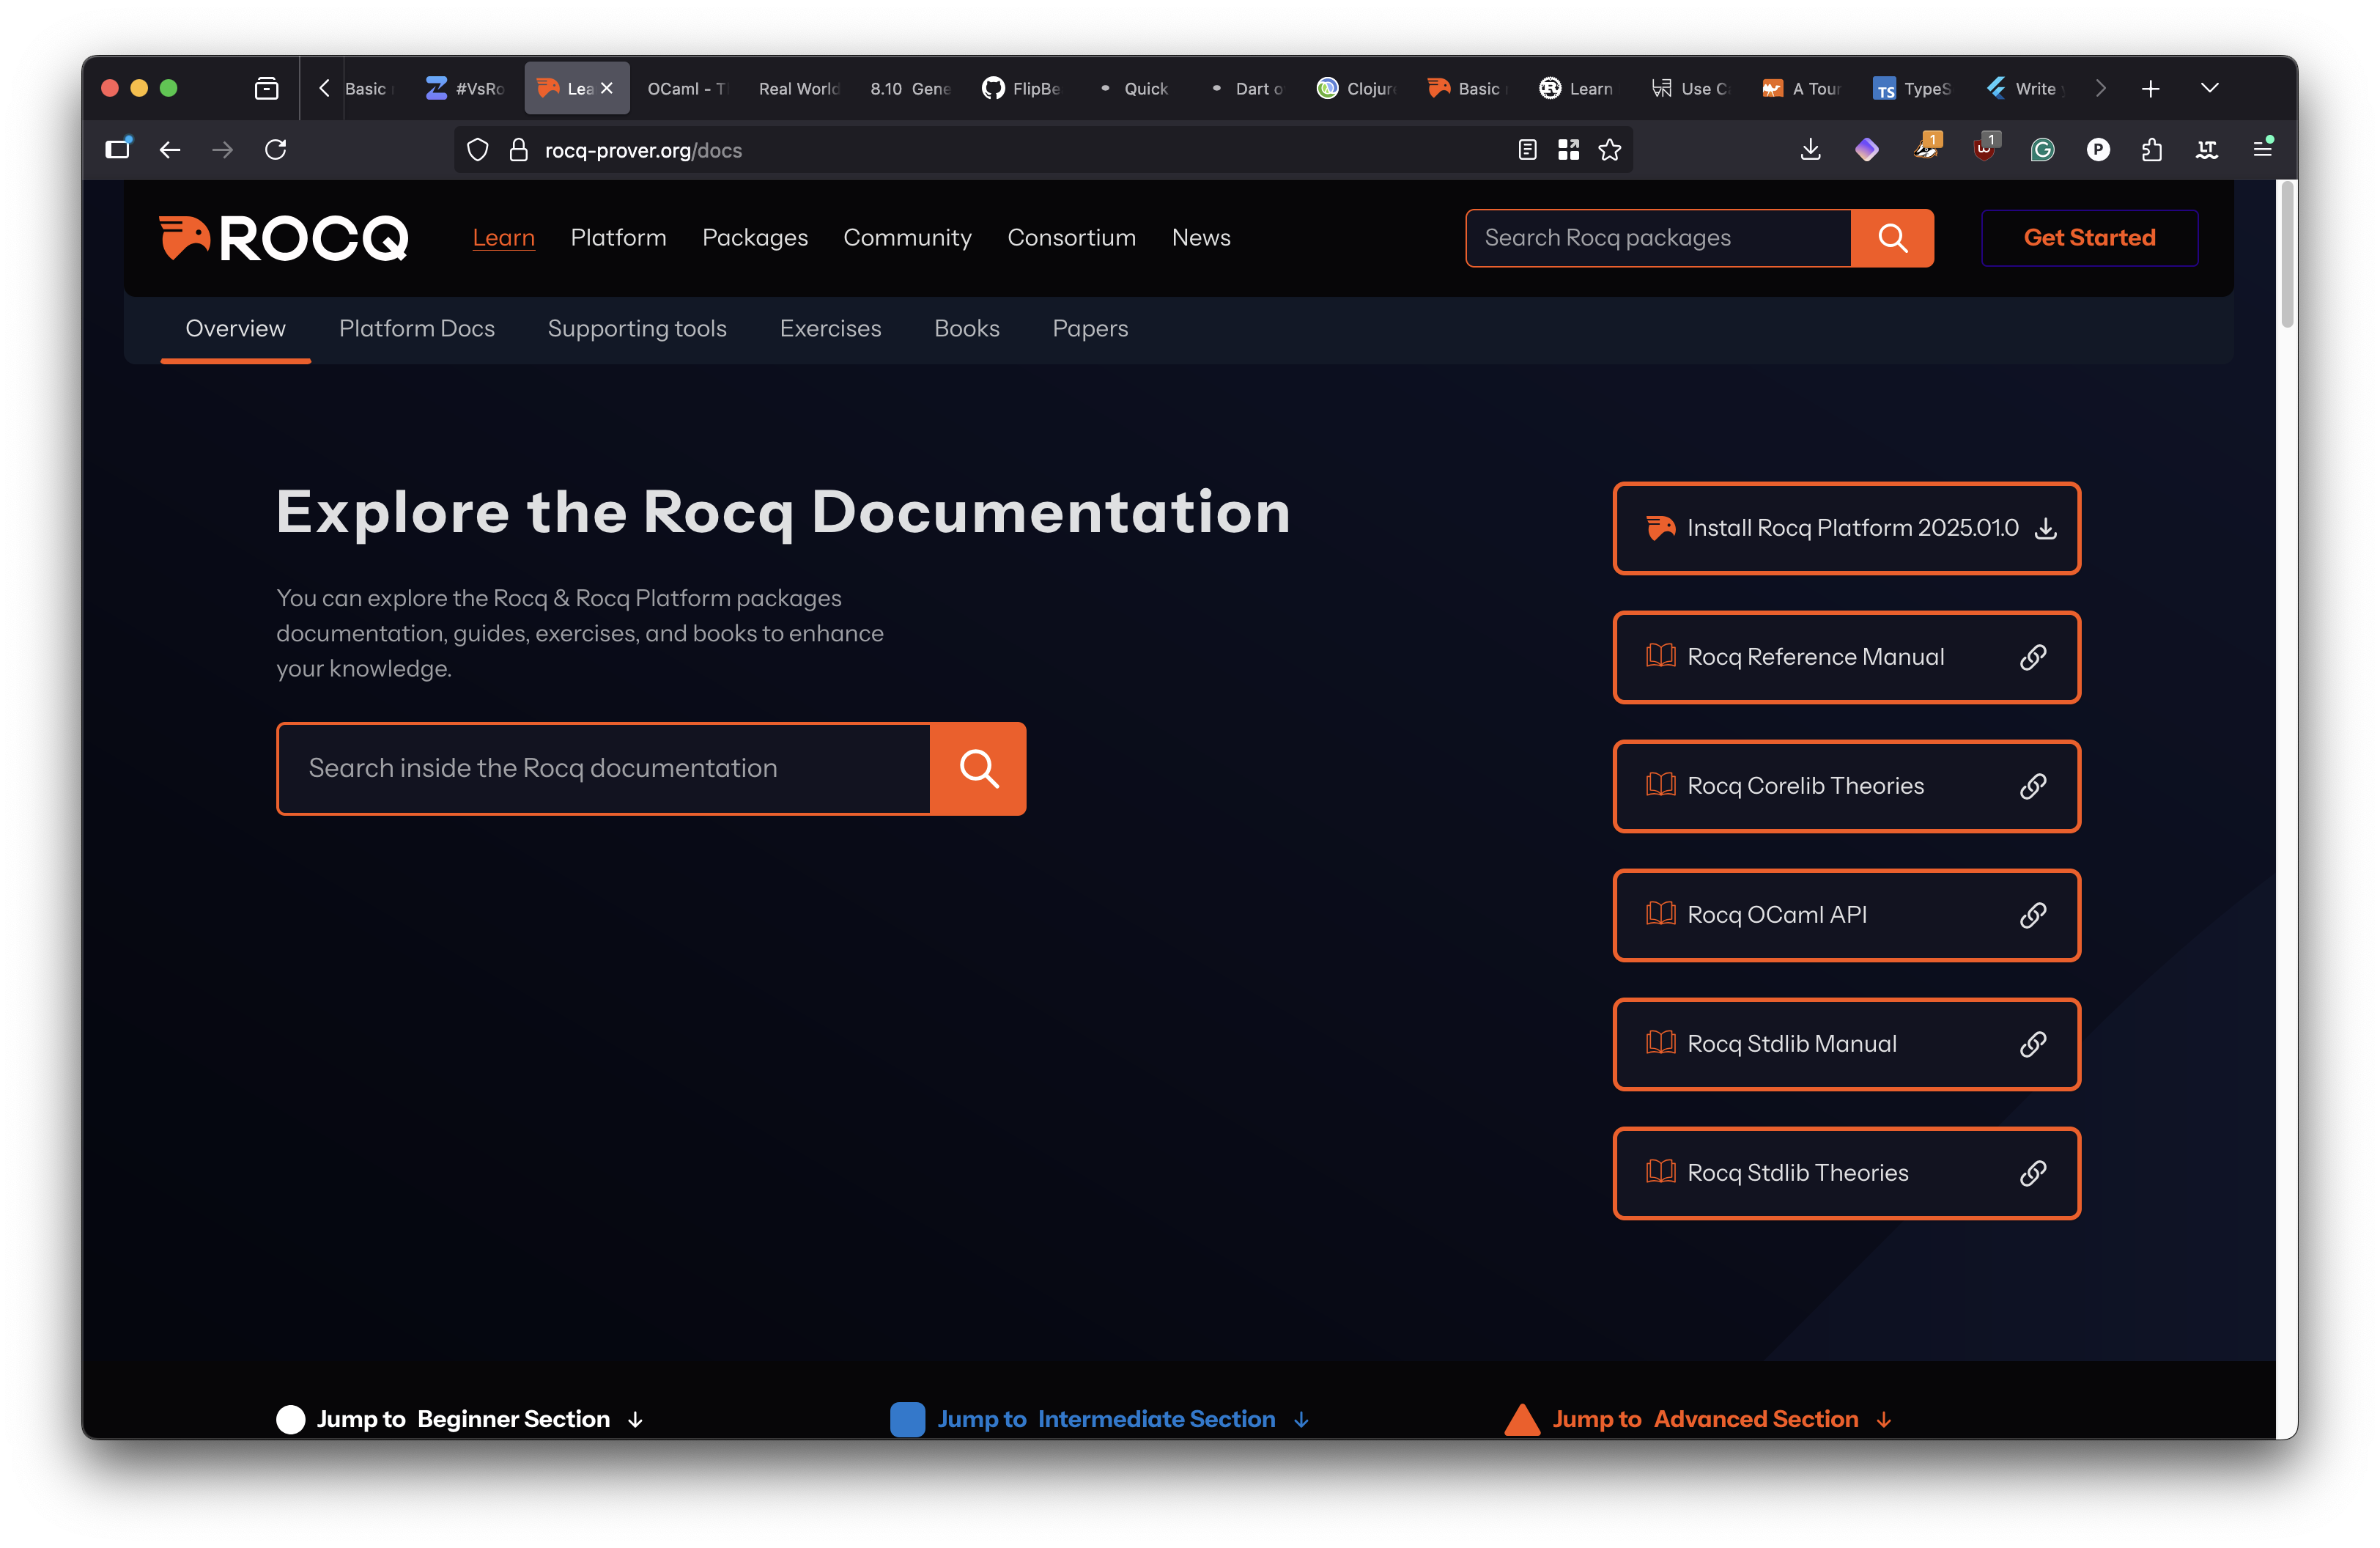
\includegraphics[width=0.45\textwidth]{rocq/doc.png}
   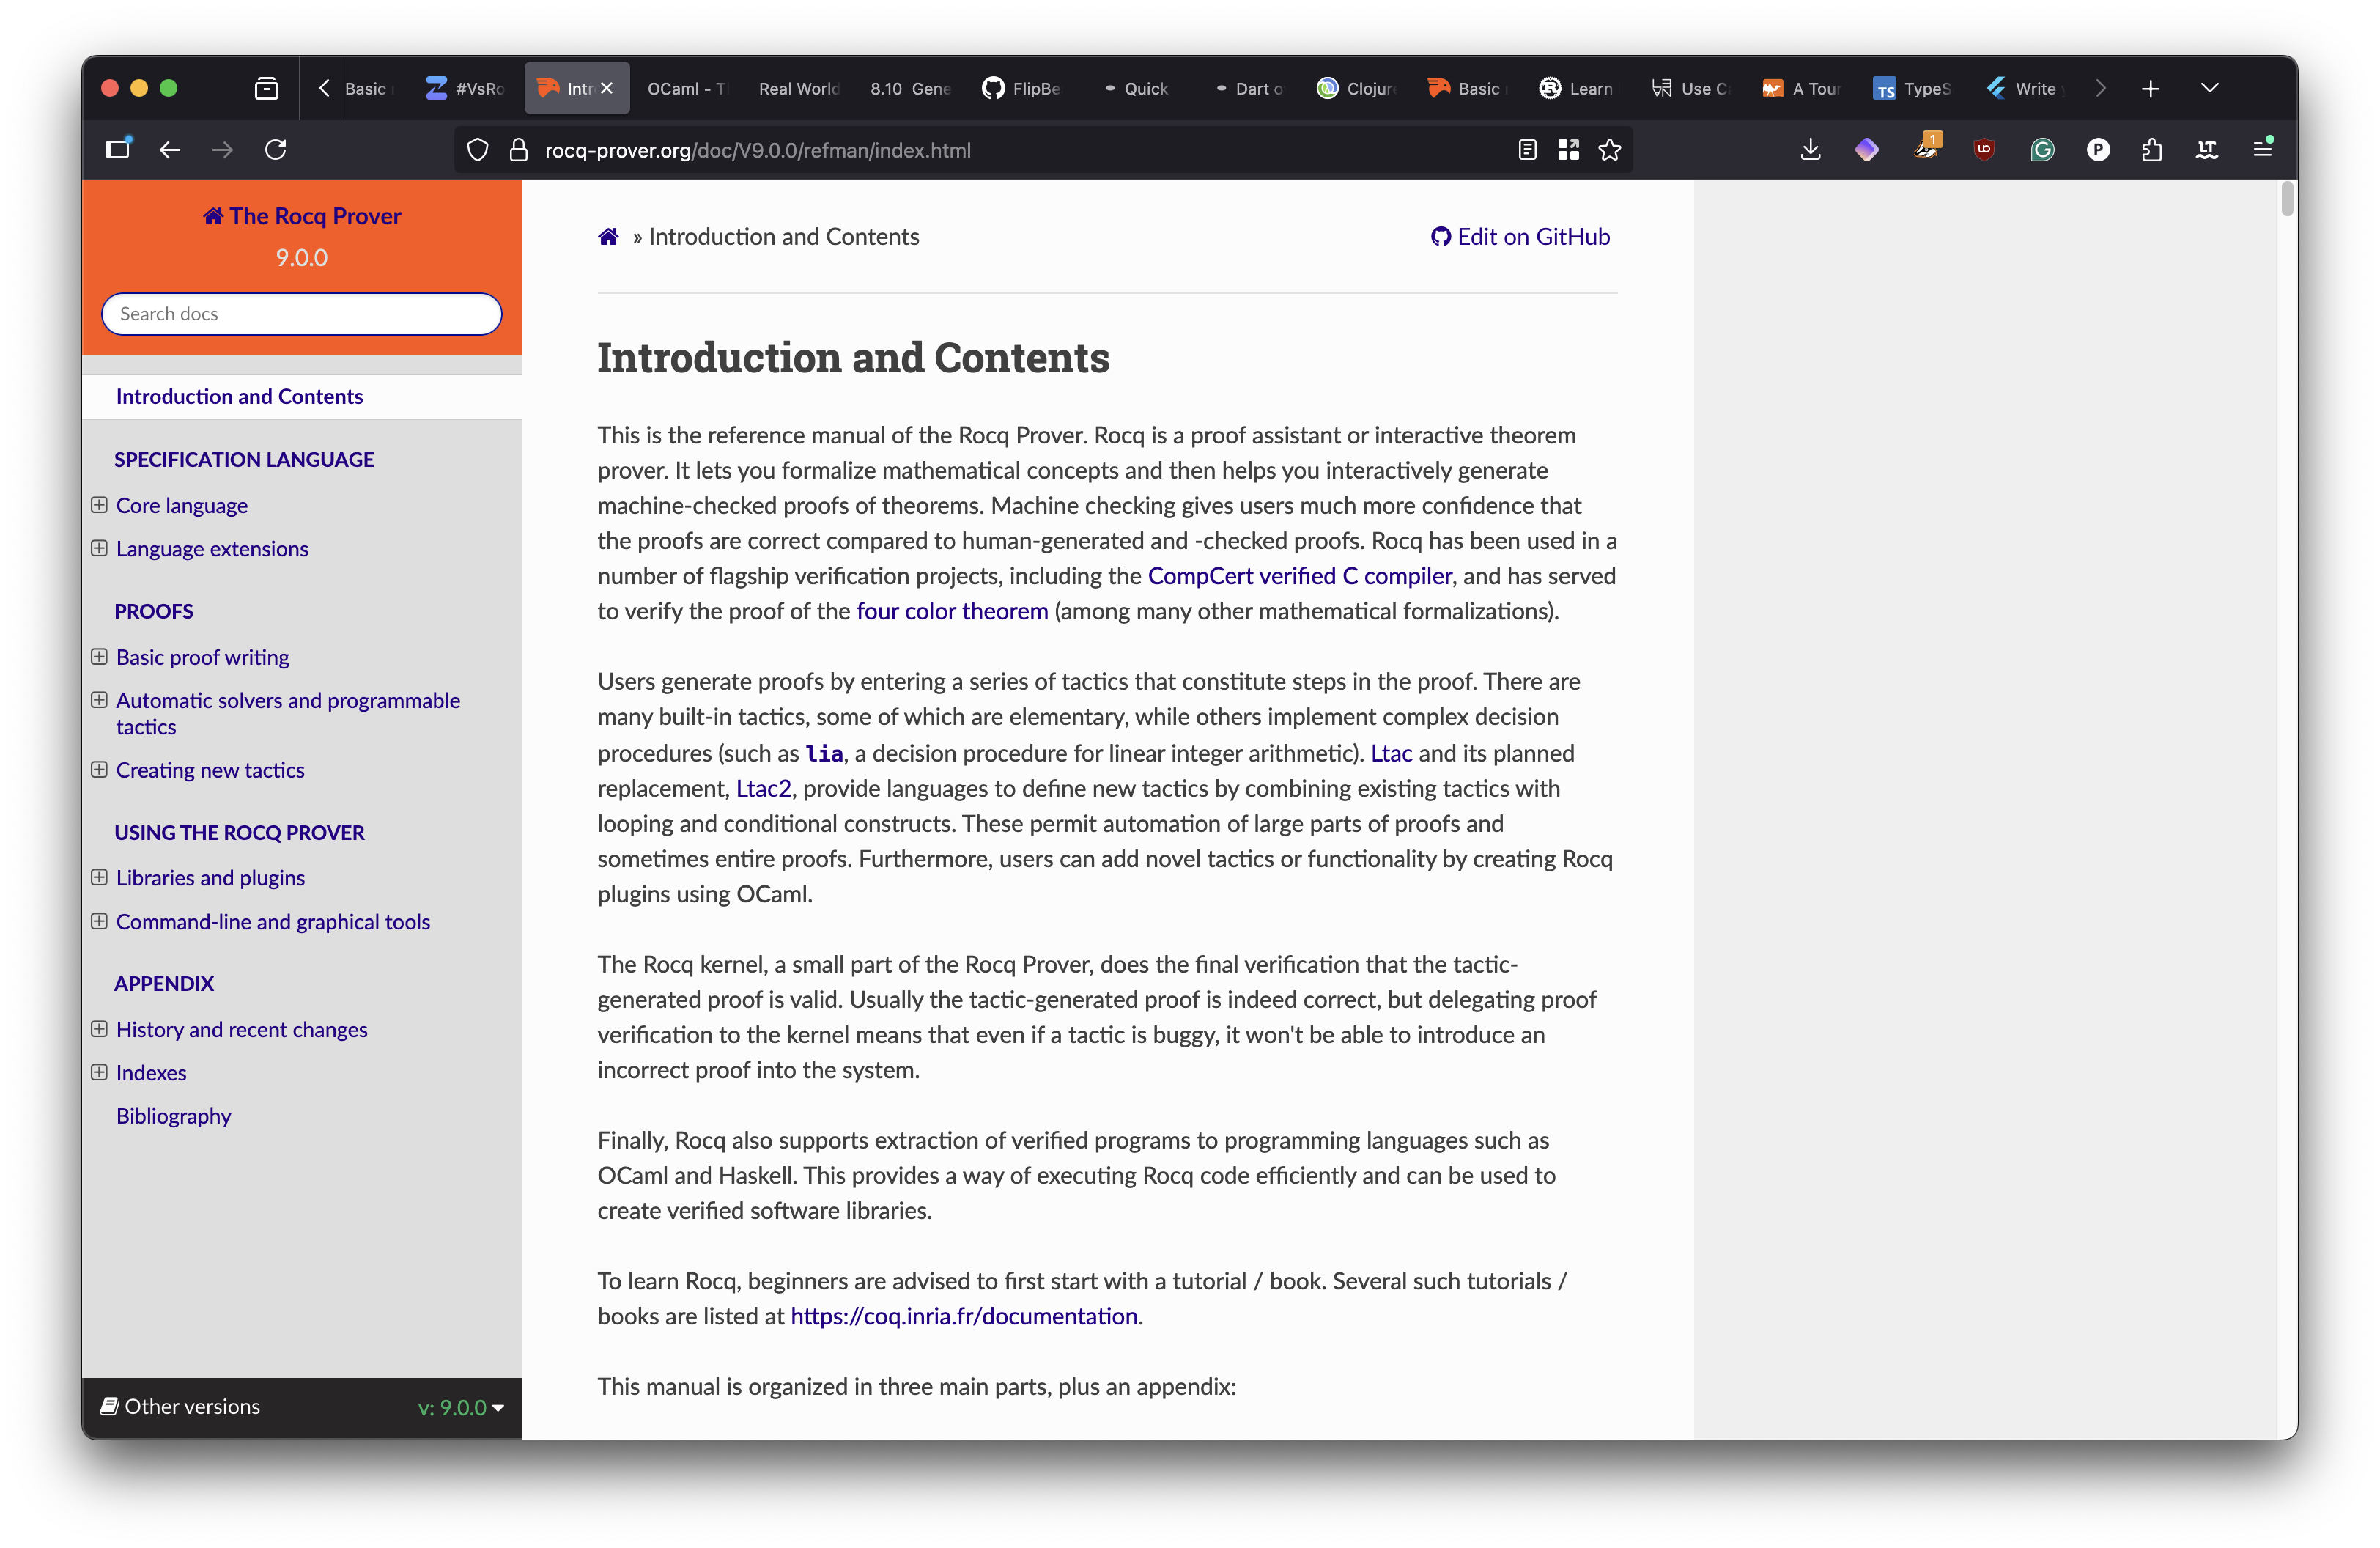
\includegraphics[width=0.45\textwidth]{rocq/manual.png}
\end{frame}

\begin{frame}{This should be more visible}
   \centering
   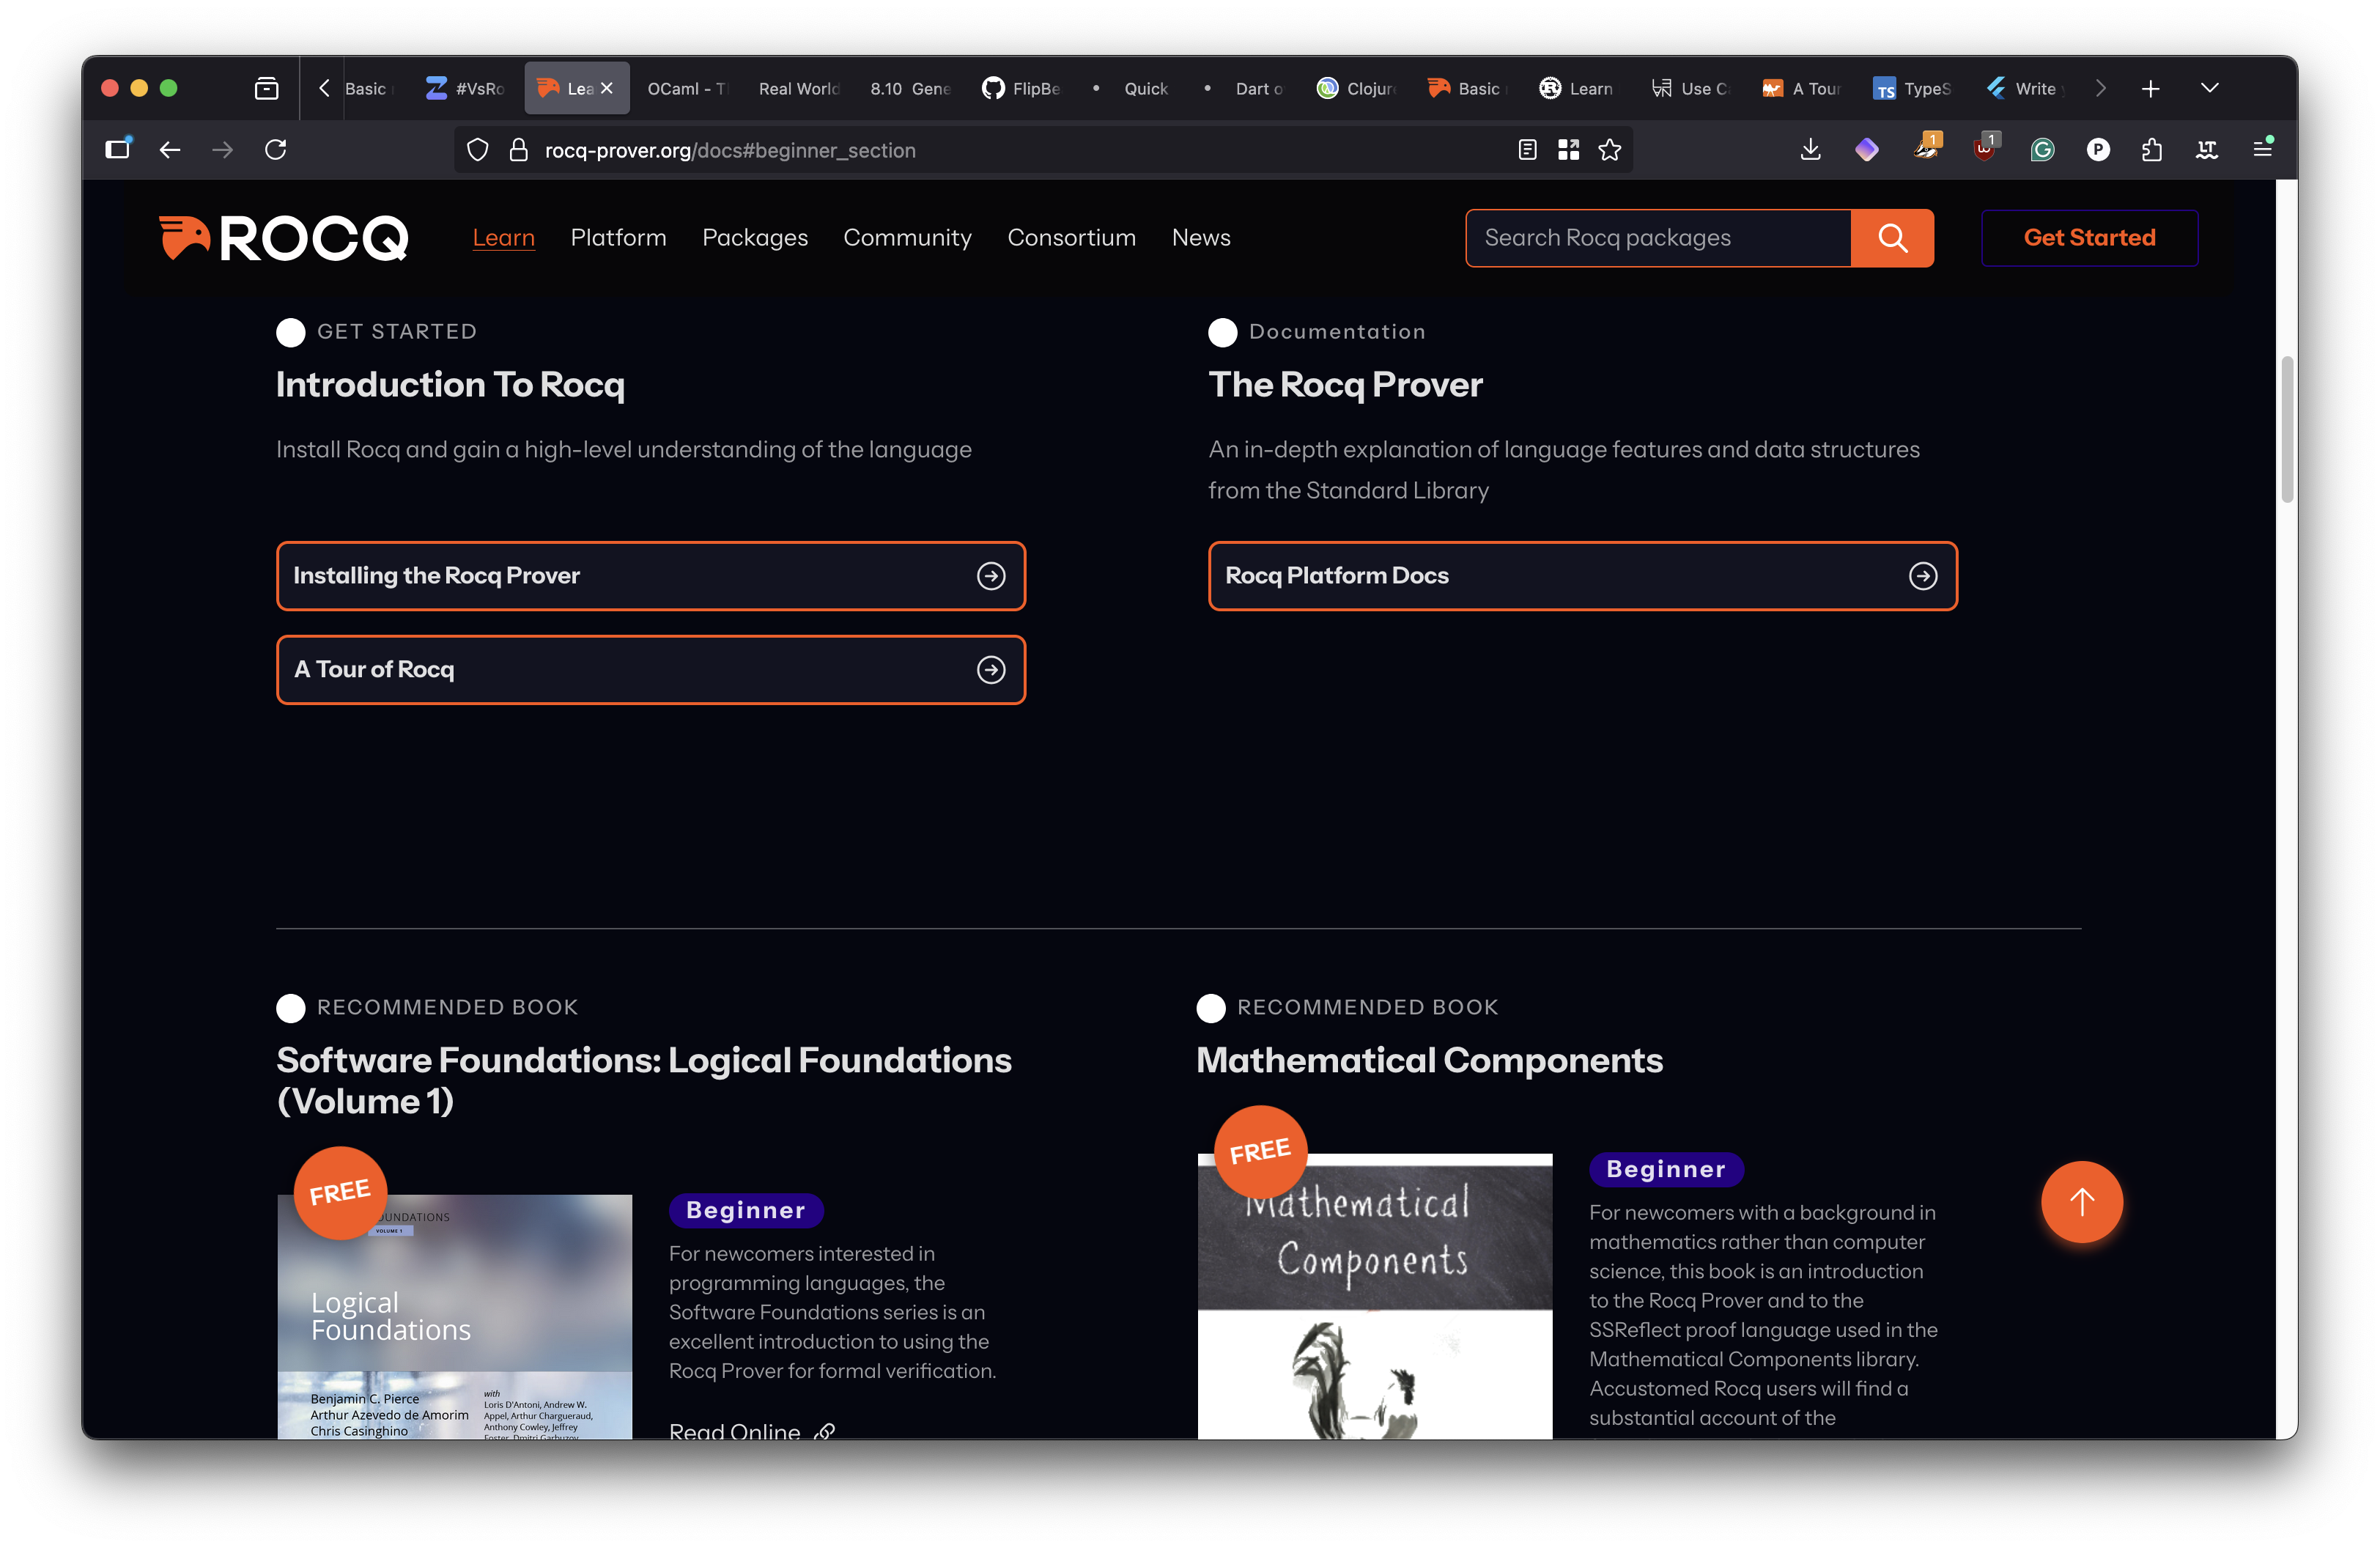
\includegraphics[width=0.45\textwidth]{rocq2/getstart.png}
   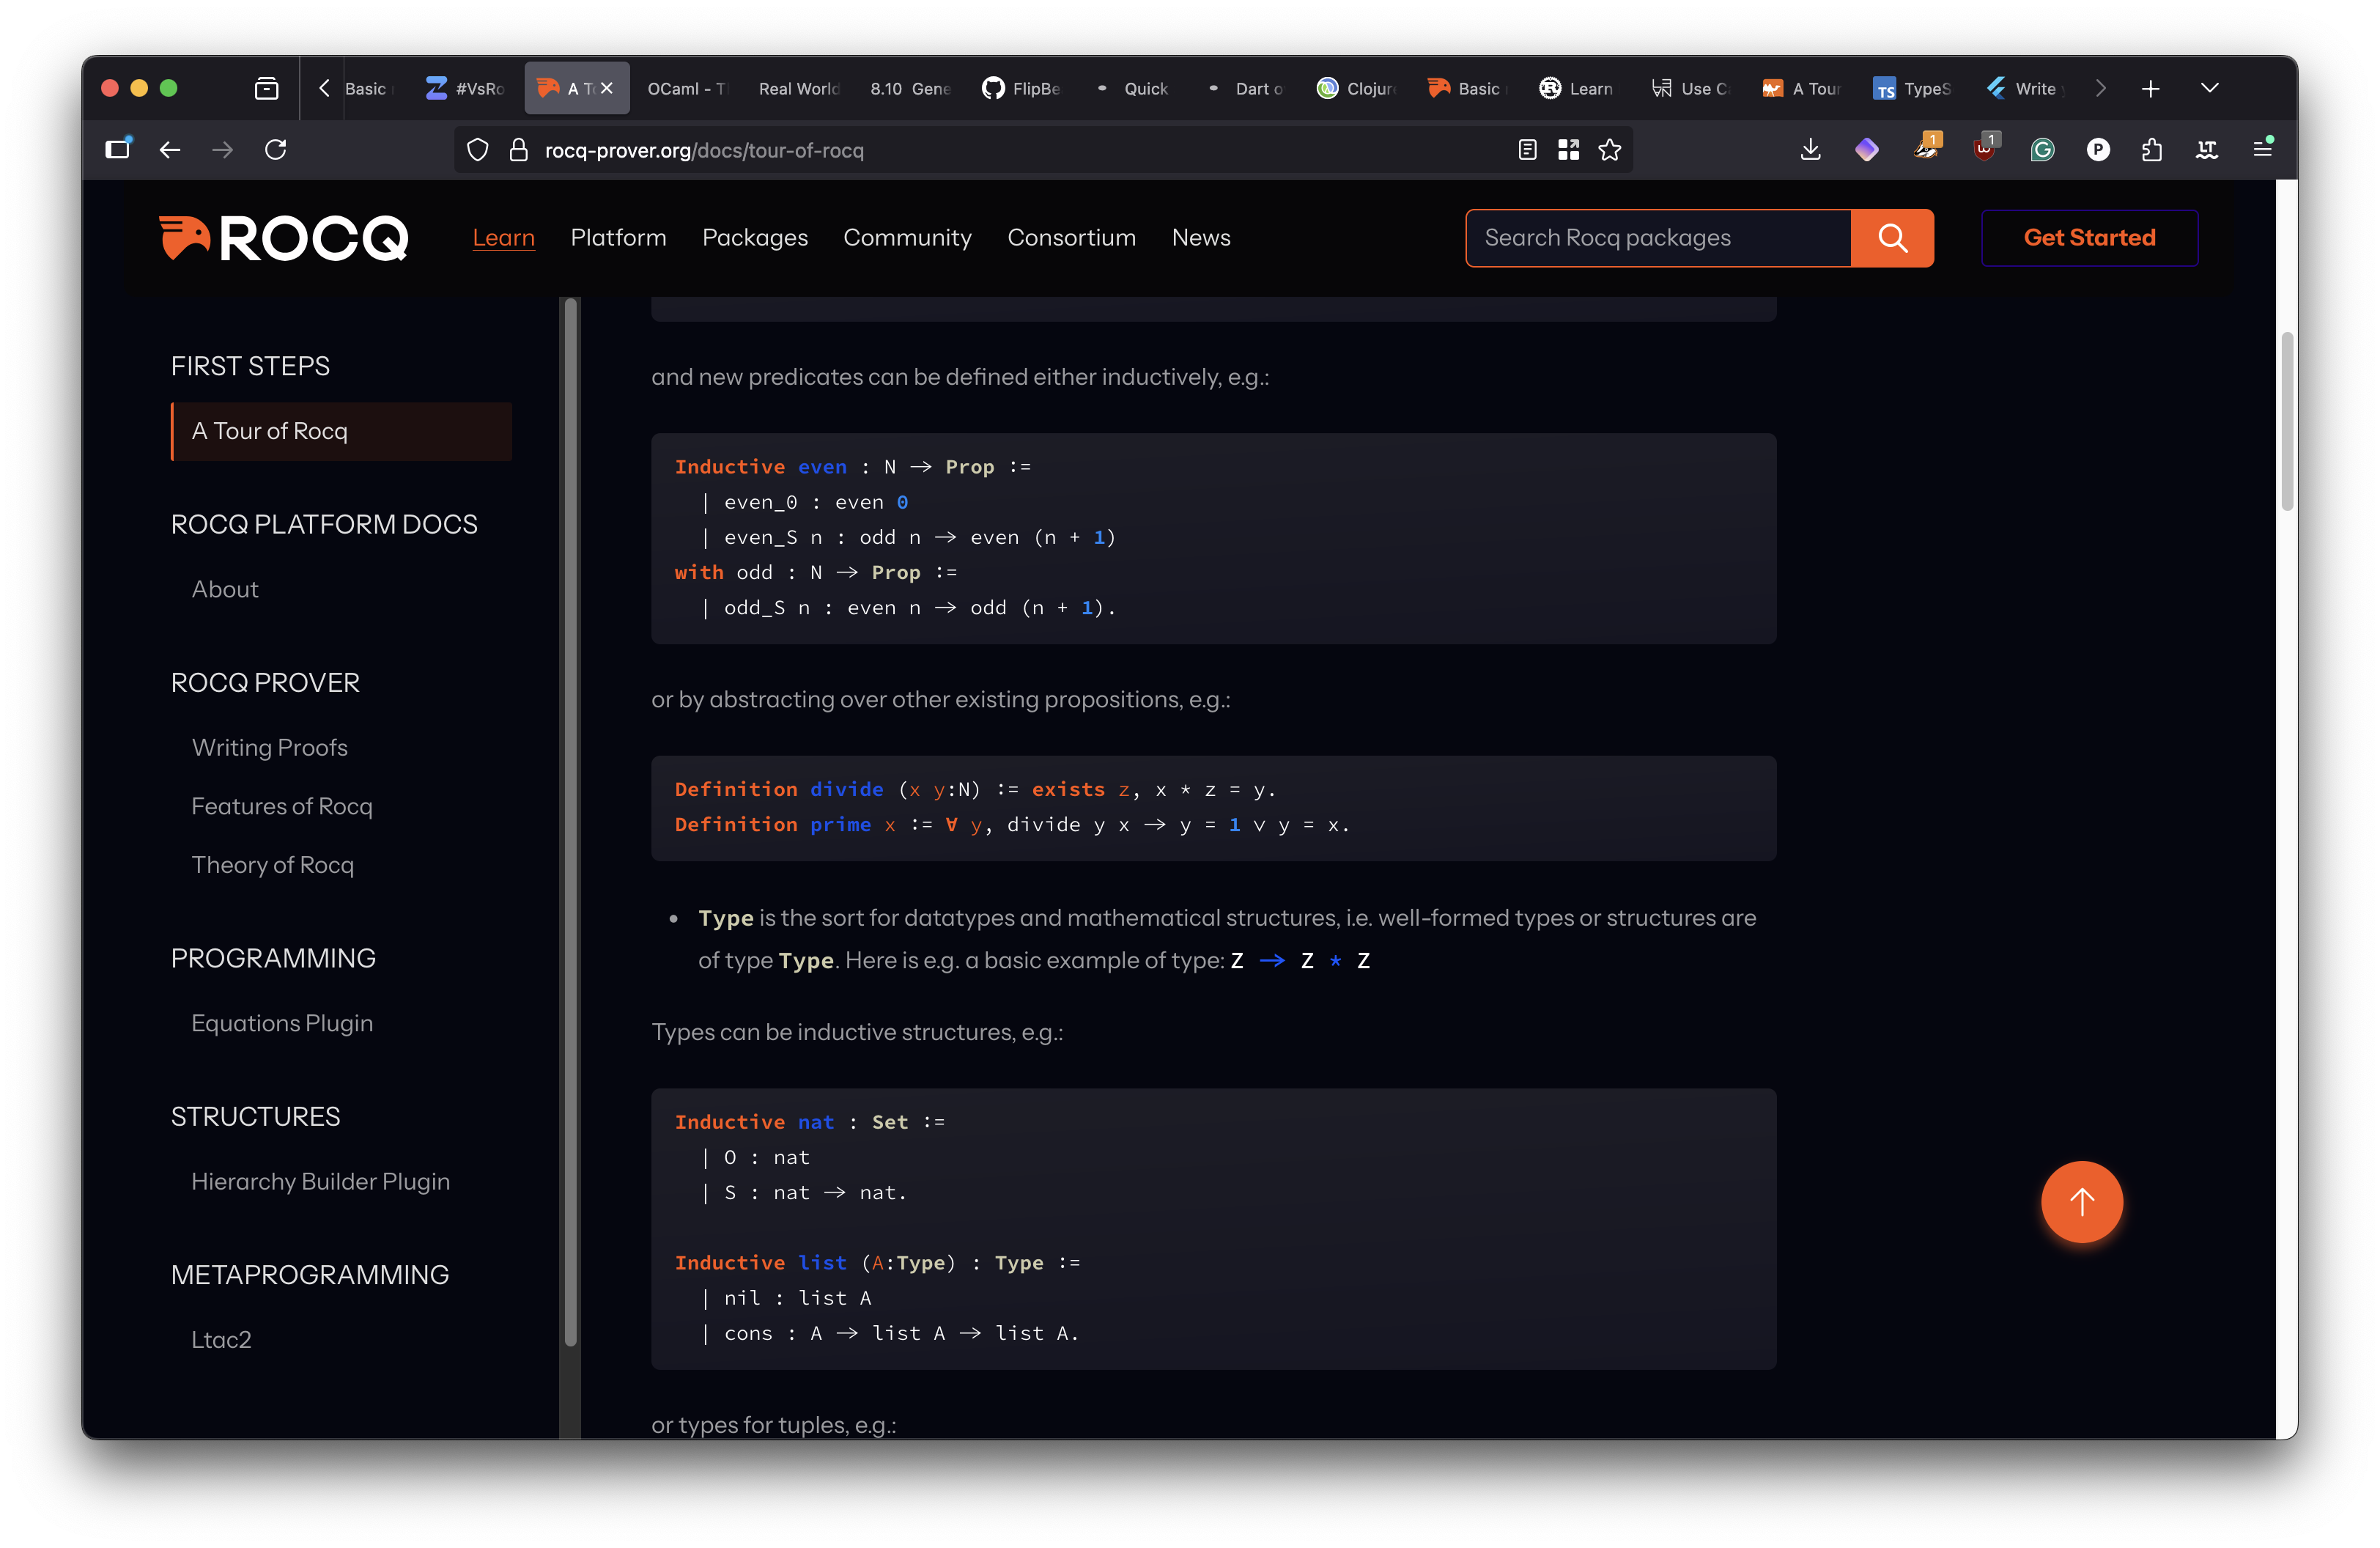
\includegraphics[width=0.45\textwidth]{rocq2/example.png}

   Ended up using Software Foundations Vol. 1
   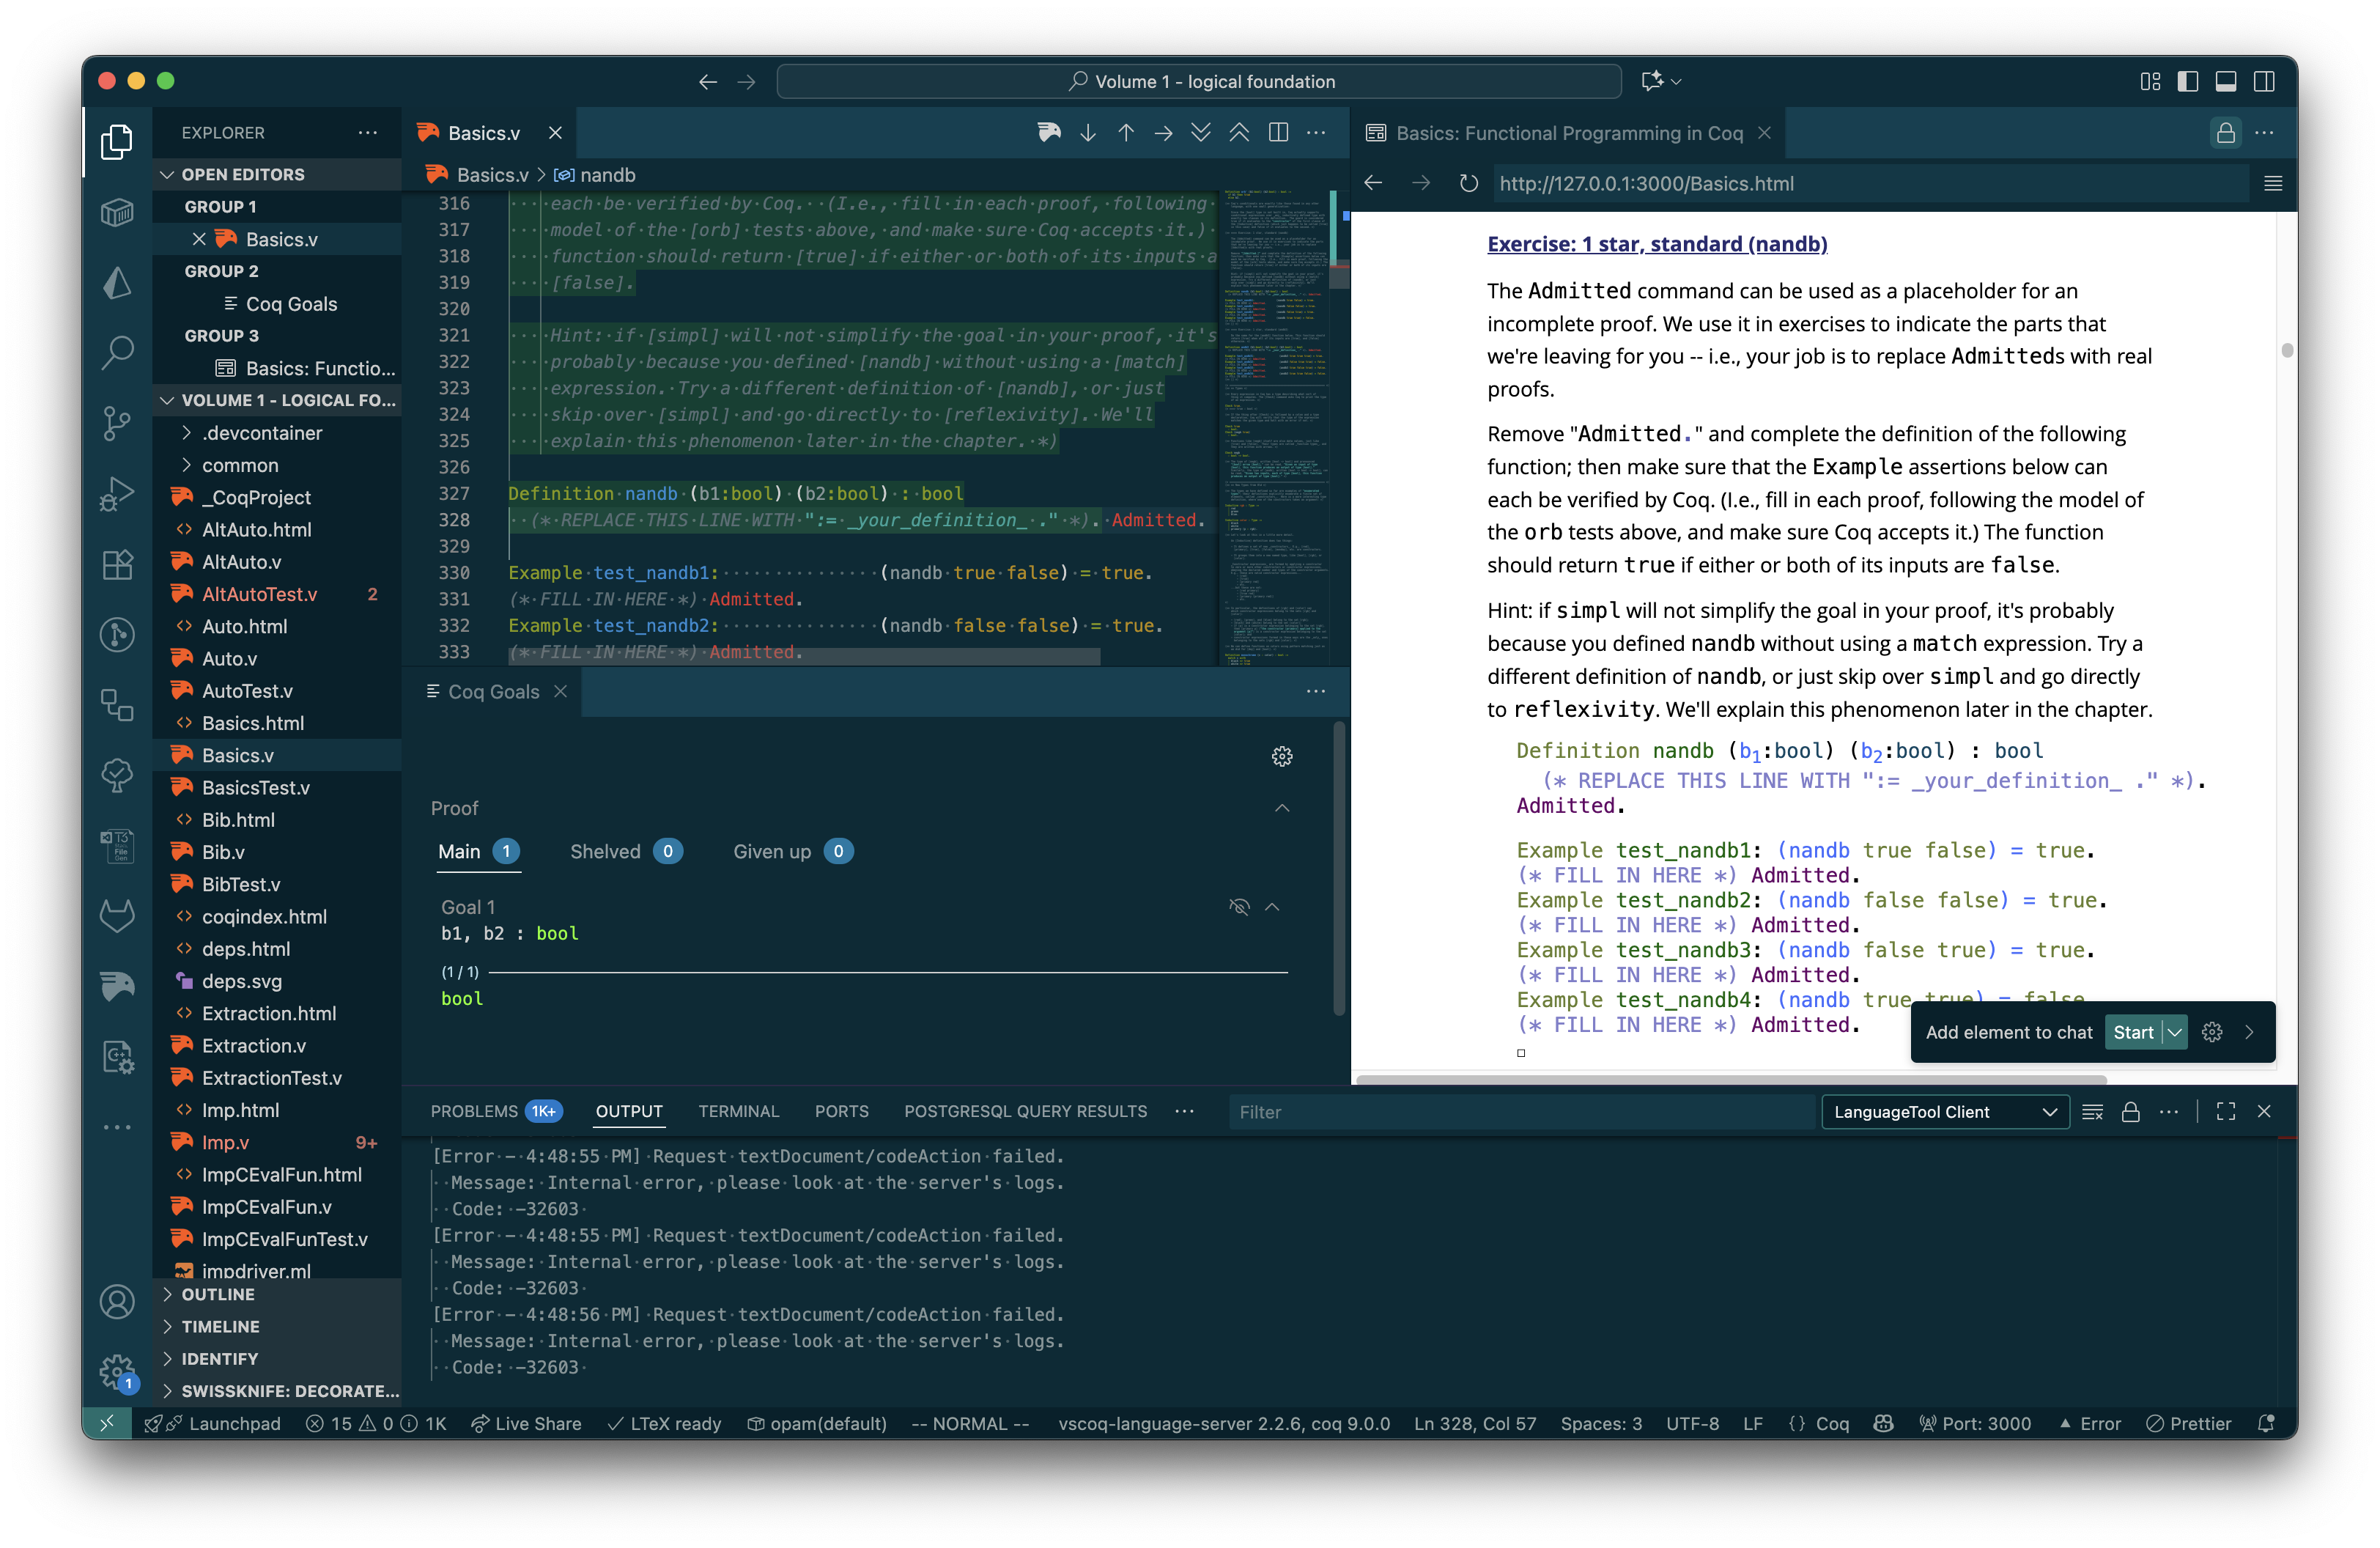
\includegraphics[width=\textwidth]{sf-lf/image.png}

\end{frame}

\section{\scshape Hands-on Experience}

%-------------------
\begin{frame}{Case Study: Red-Black Tree Deletion}
   \begin{block}{what ?}
      Well-know data structure
   \end{block}
   \begin{block}{why ?}
      Could not find an existing implem or proof
   \end{block}

\end{frame}

%-------------------
\begin{frame}{Seems simple}
   \begin{itemize}
      \item Fairly simple structure

            \begin{center}
               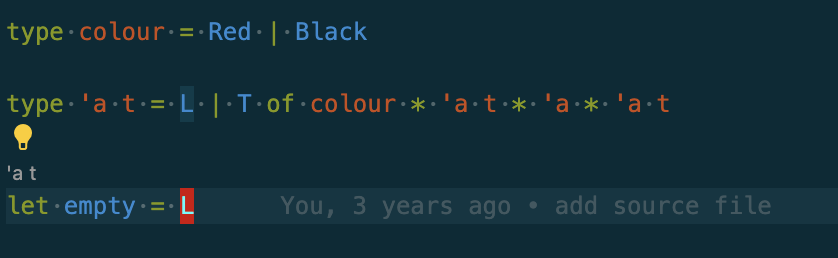
\includegraphics[width=0.5\textwidth]{ocaml-code/image.png}
            \end{center}

      \item Fairly simple algorithm (about 100 lines)
      \item Fairly simple properties to express

            \begin{center}
               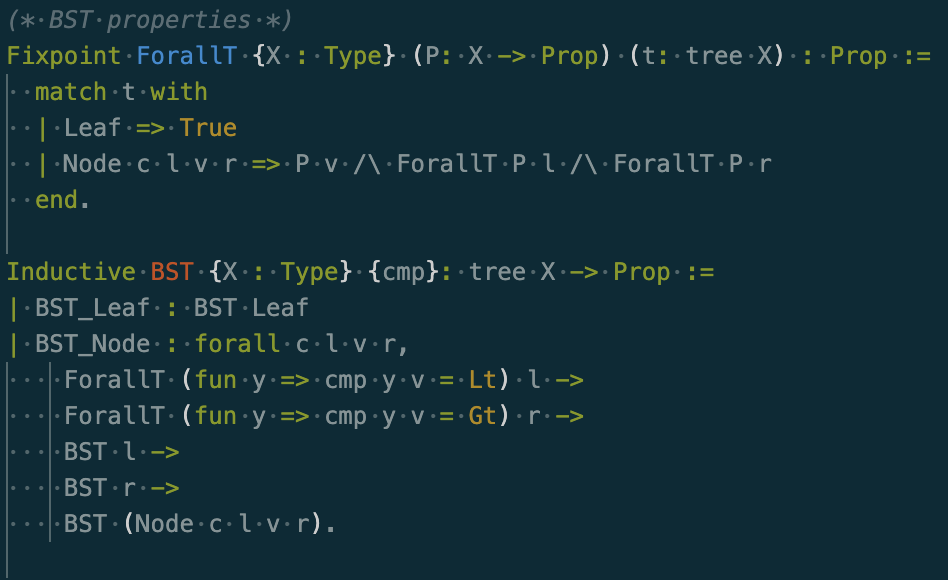
\includegraphics[width=0.45\textwidth]{coq-code/bst.png}
               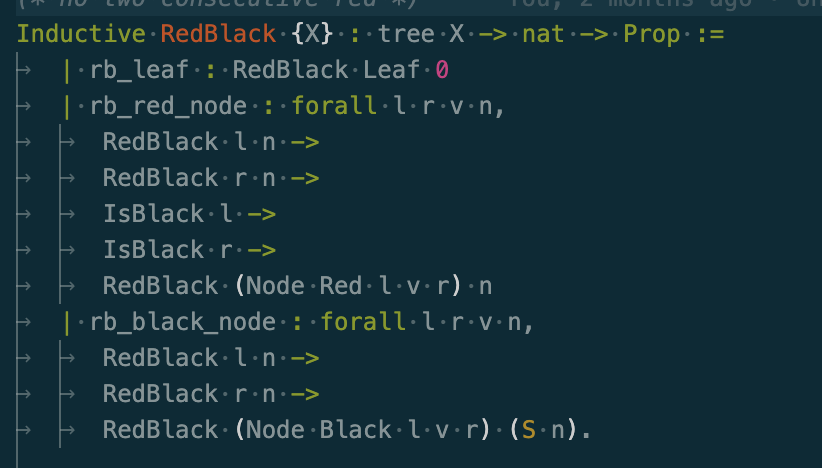
\includegraphics[width=0.45\textwidth]{coq-code/redblack.png}
            \end{center}

      \item Fairlty simple theorem
            \begin{center}
               
\includegraphics[width=0.8\textwidth]{coq-code/theorem.png}
            \end{center}
   \end{itemize}
\end{frame}

\begin{frame}{Already made an informal explanation ! (proof ?)}
   \begin{center}
      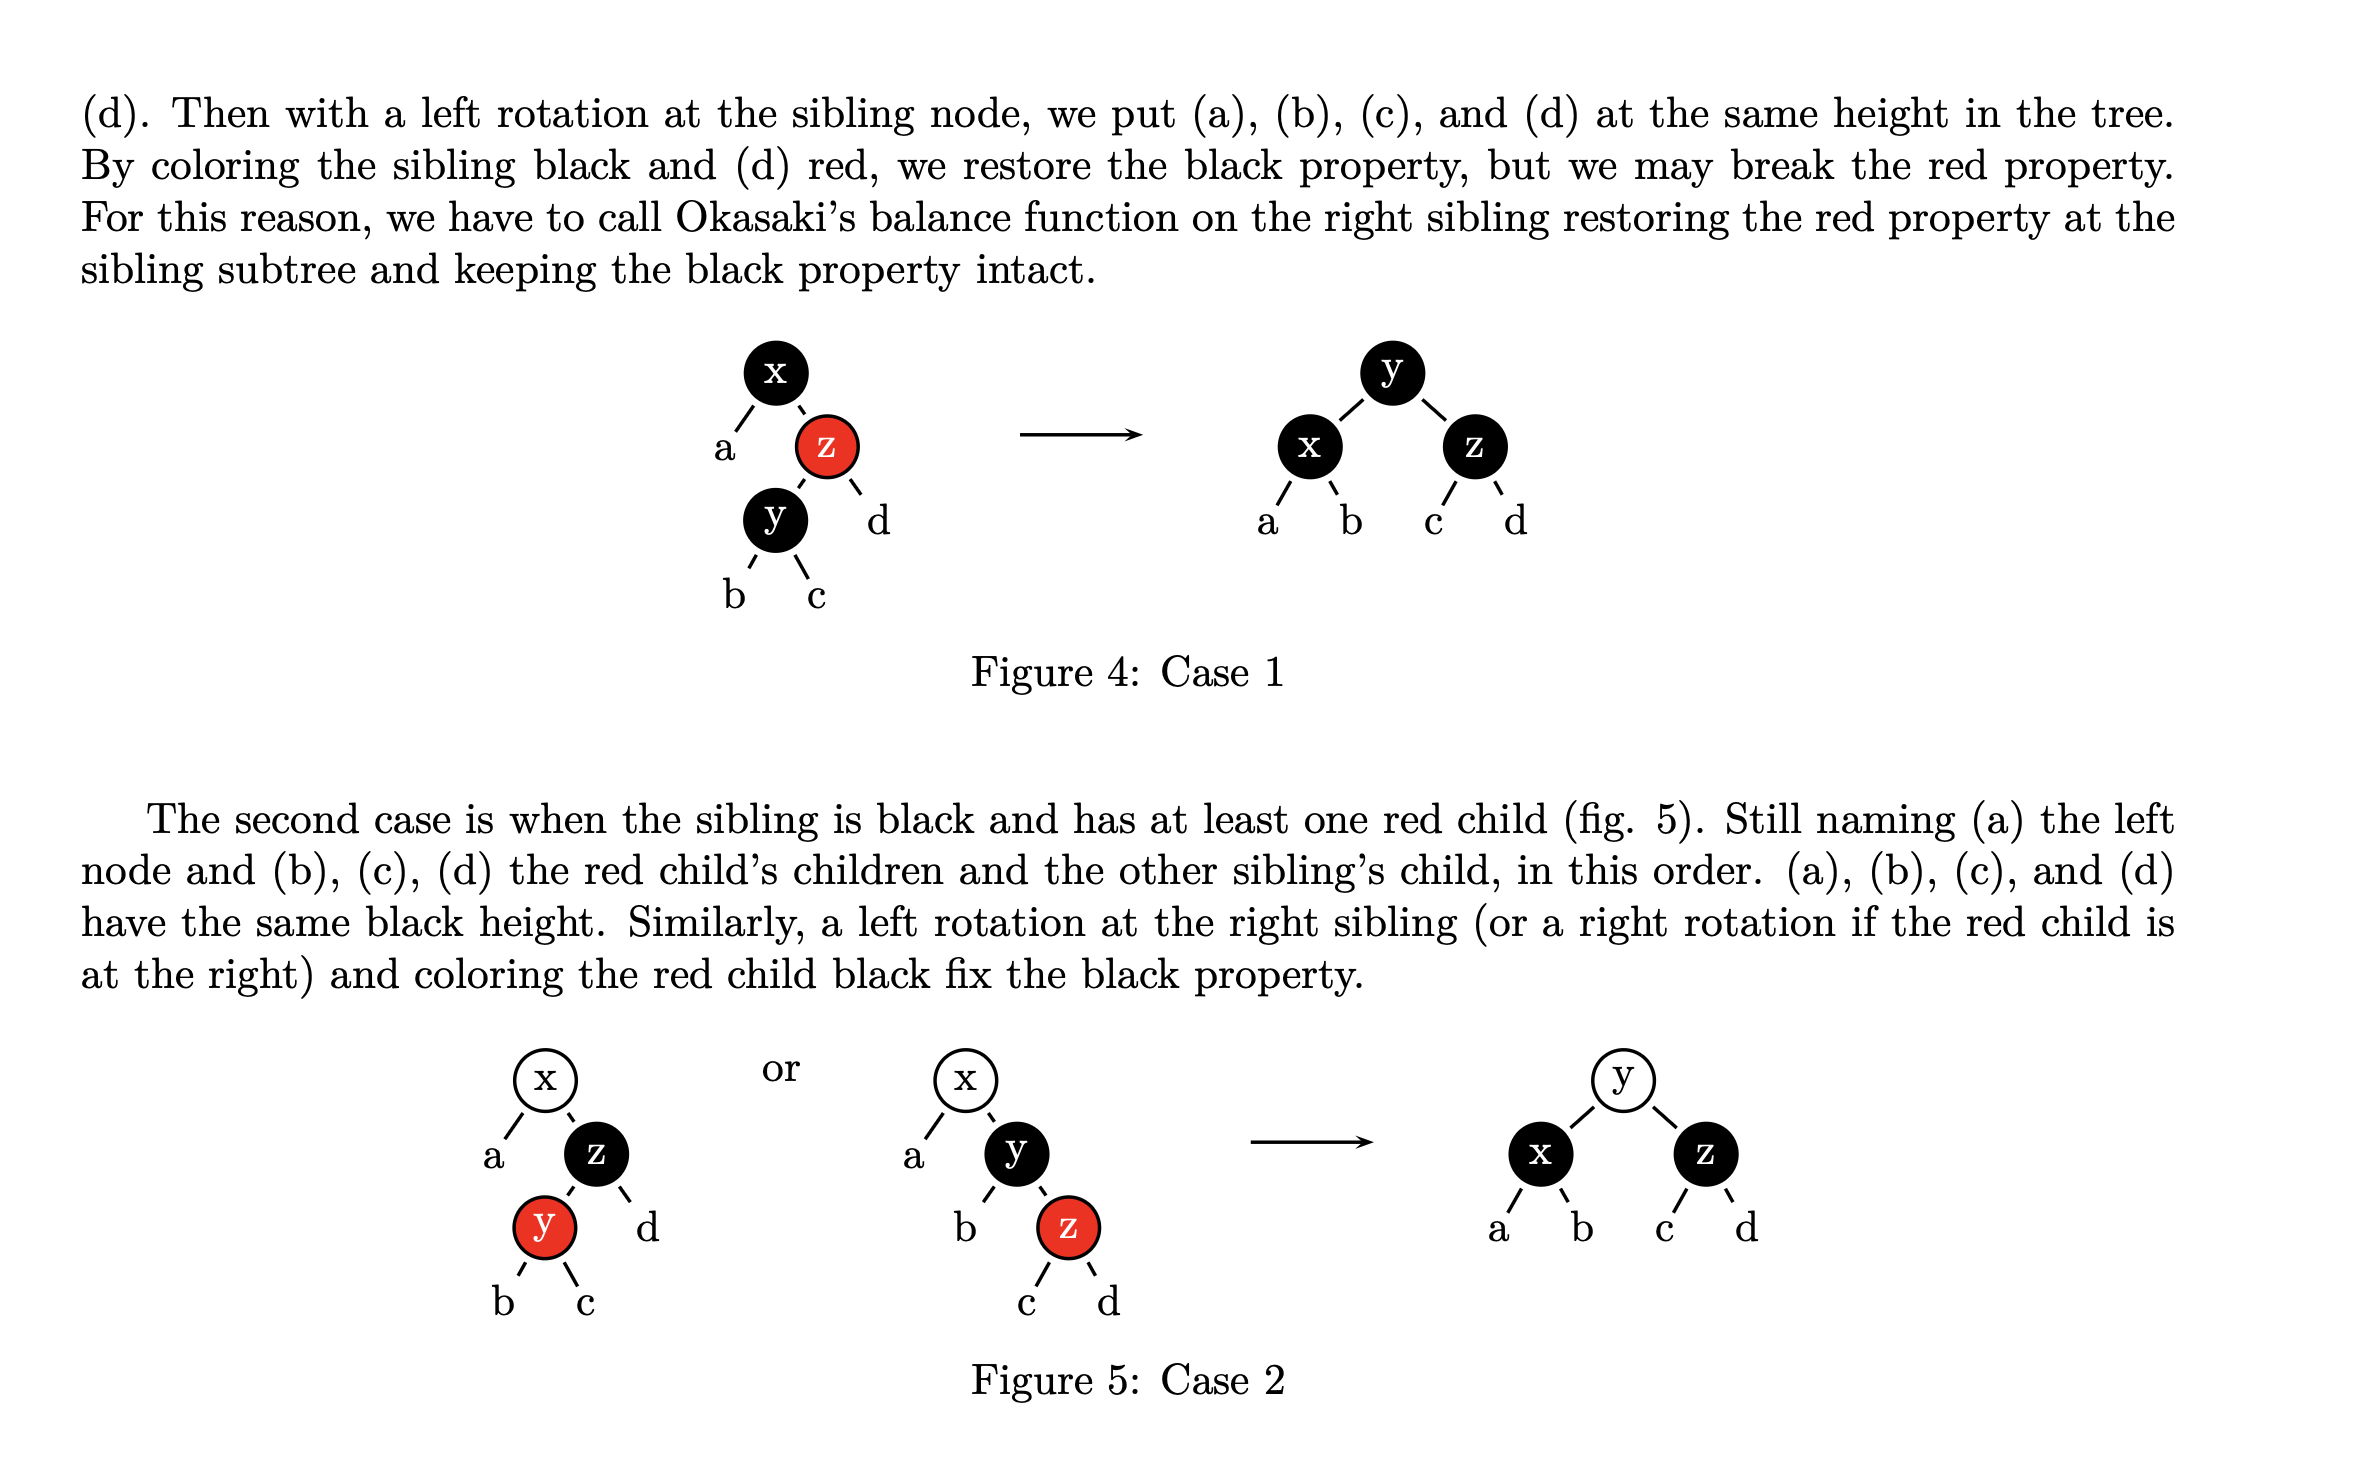
\includegraphics[width=0.9\textwidth]{paper-proof/image.png}
   \end{center}
\end{frame}

\begin{frame}{Reality: Big chunky proof}

   Attempting to prove insertion first and failing

   \vspace{1em}
   \centering
   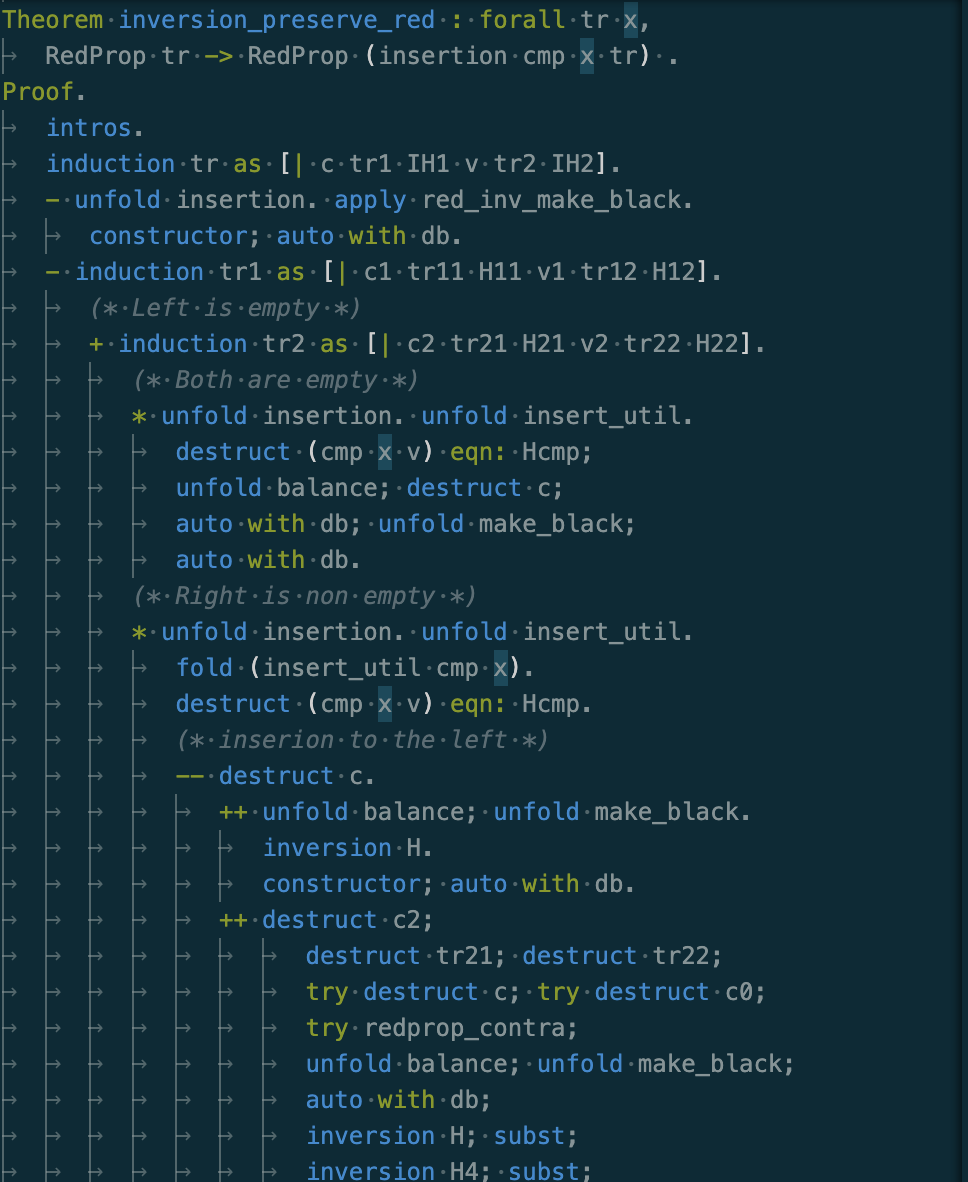
\includegraphics[width=0.3\textwidth]{attempt1/1.png}
   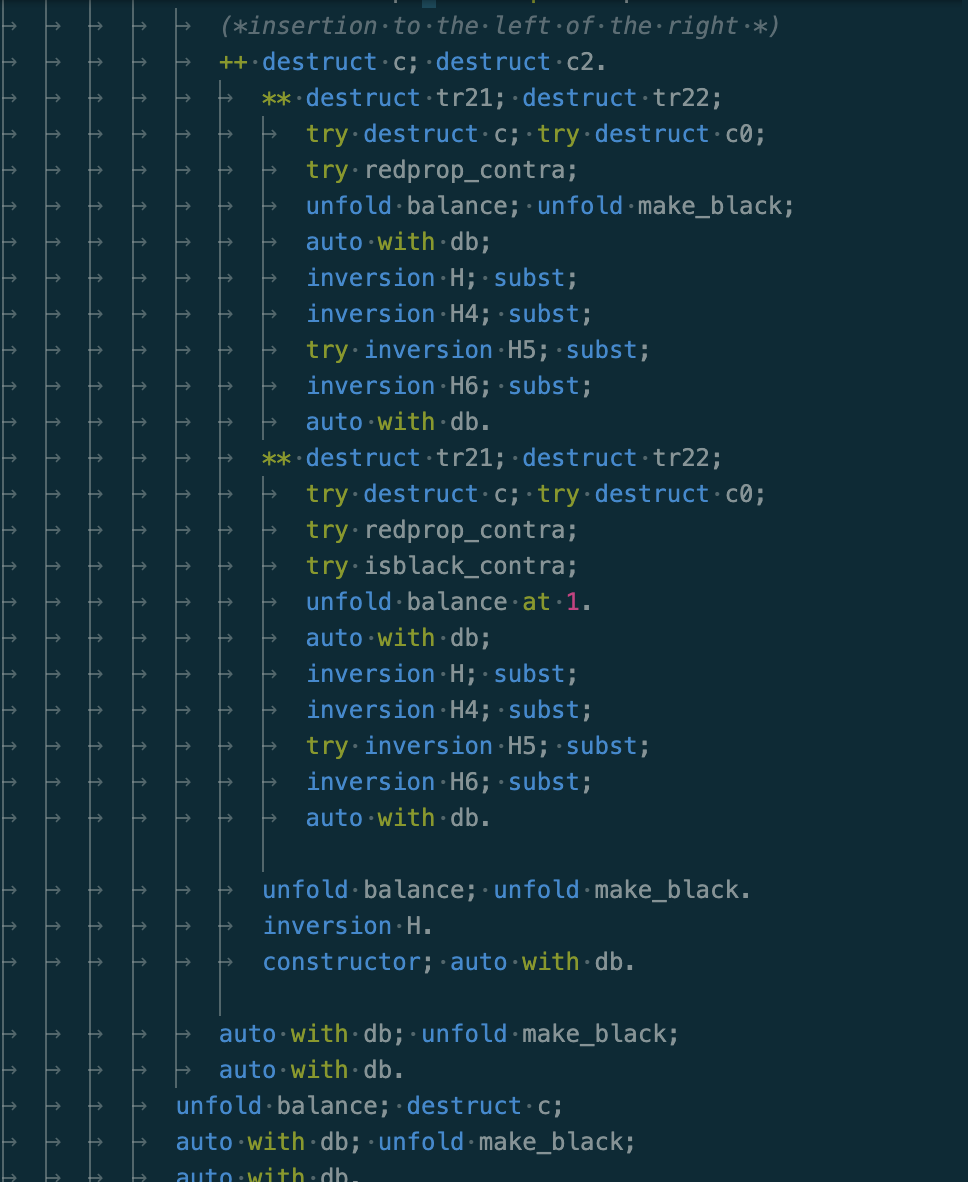
\includegraphics[width=0.3\textwidth]{attempt1/2.png}
   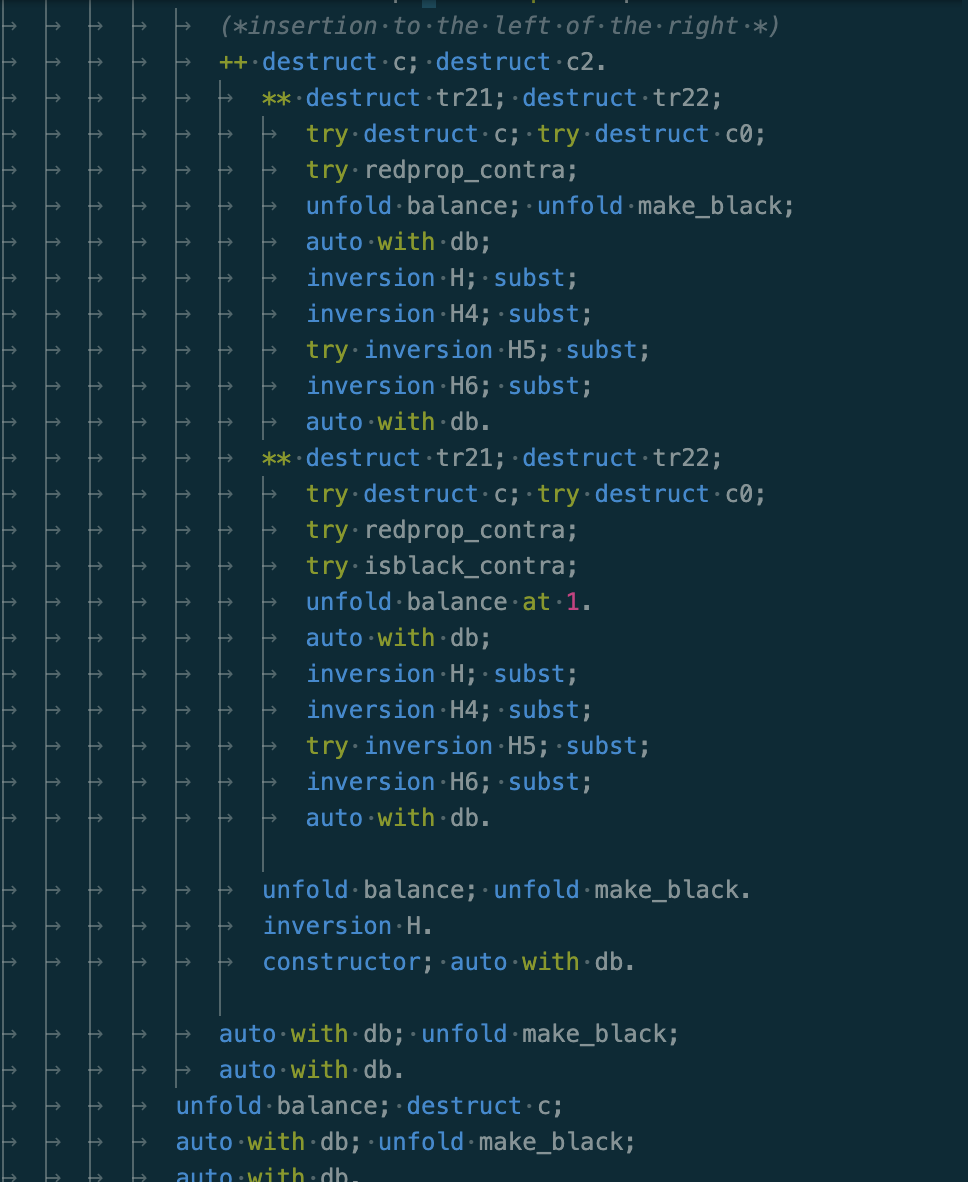
\includegraphics[width=0.3\textwidth]{attempt1/3.png}
   % Proof state screenshot placeholder:
   % \includegraphics[width=0.8\textwidth]{messy-proof.png}
\end{frame}

%-------------------
\begin{frame}{Read Soft Found 3. and retry}
   intermediary data structures
   \begin{center}
      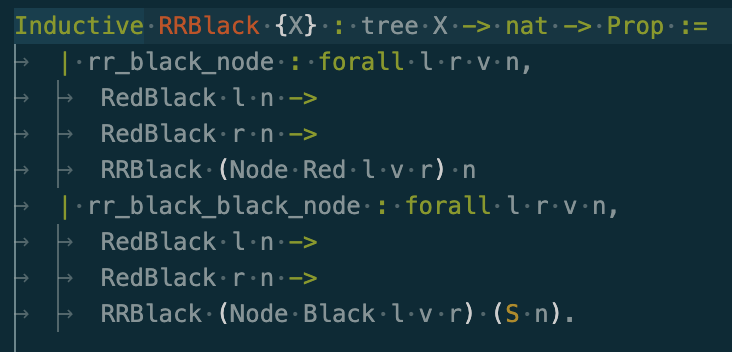
\includegraphics[width=0.45\textwidth]{attempt2/1.png}
   \end{center}
   use of ltac(1) for automation
   \vspace{1em}

   \centering
   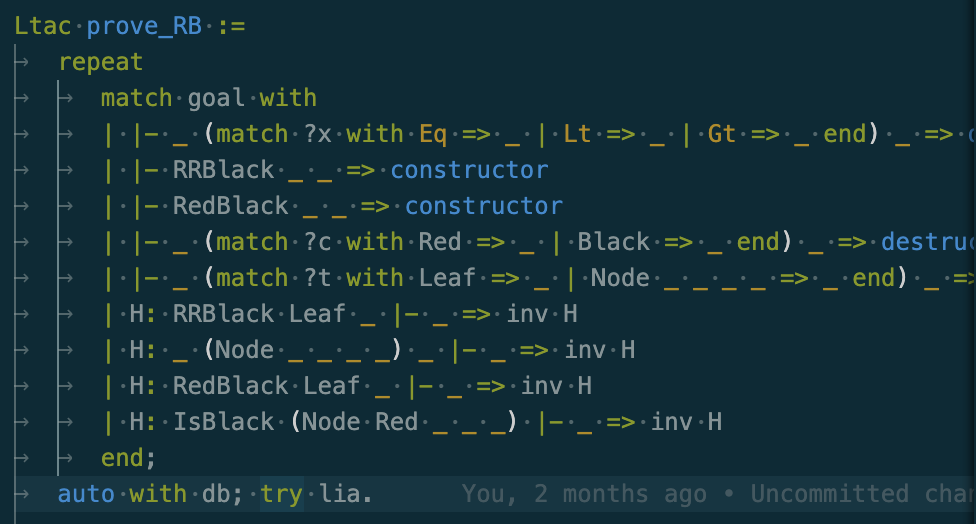
\includegraphics[width=0.45\textwidth]{attempt2/2.png}
\end{frame}

\section{\scshape Reflections}
%-------------------
\begin{frame}{Pain points}
   \begin{itemize}
      \item Proof to long ? split in smaller lemmas
      \item Lose context ? add invariants
      \item With one are correct ?
   \end{itemize}

   \vspace{1em}
   \centering
   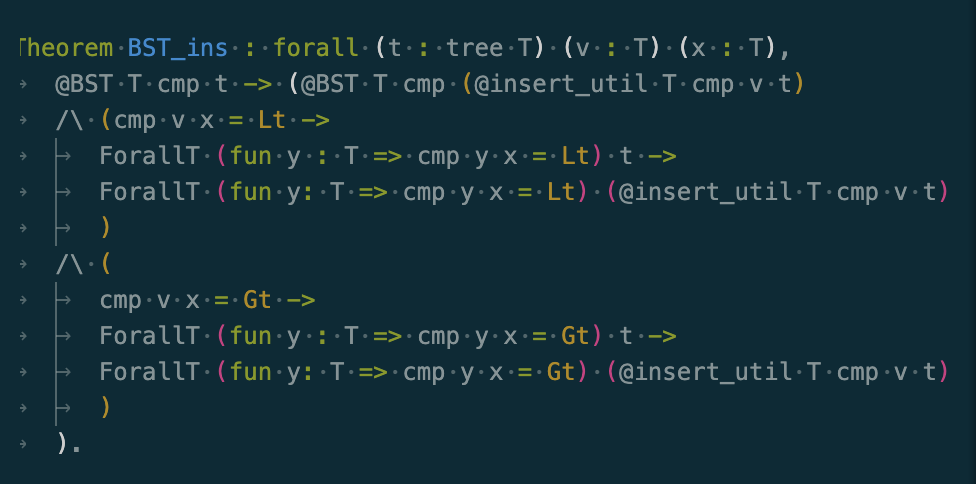
\includegraphics[width=0.45\textwidth]{pain/invariant.png}
\end{frame}

%-------------------
\begin{frame}{Pain points}
   \begin{itemize}
      \item What to do for polymorphic types ?
      \item What to do for constraints on polymorphic types ?
      \item Why does all my proofs start failing after a small change ?
   \end{itemize}
\end{frame}

\begin{frame}{Catch All tactics}
   \centering
   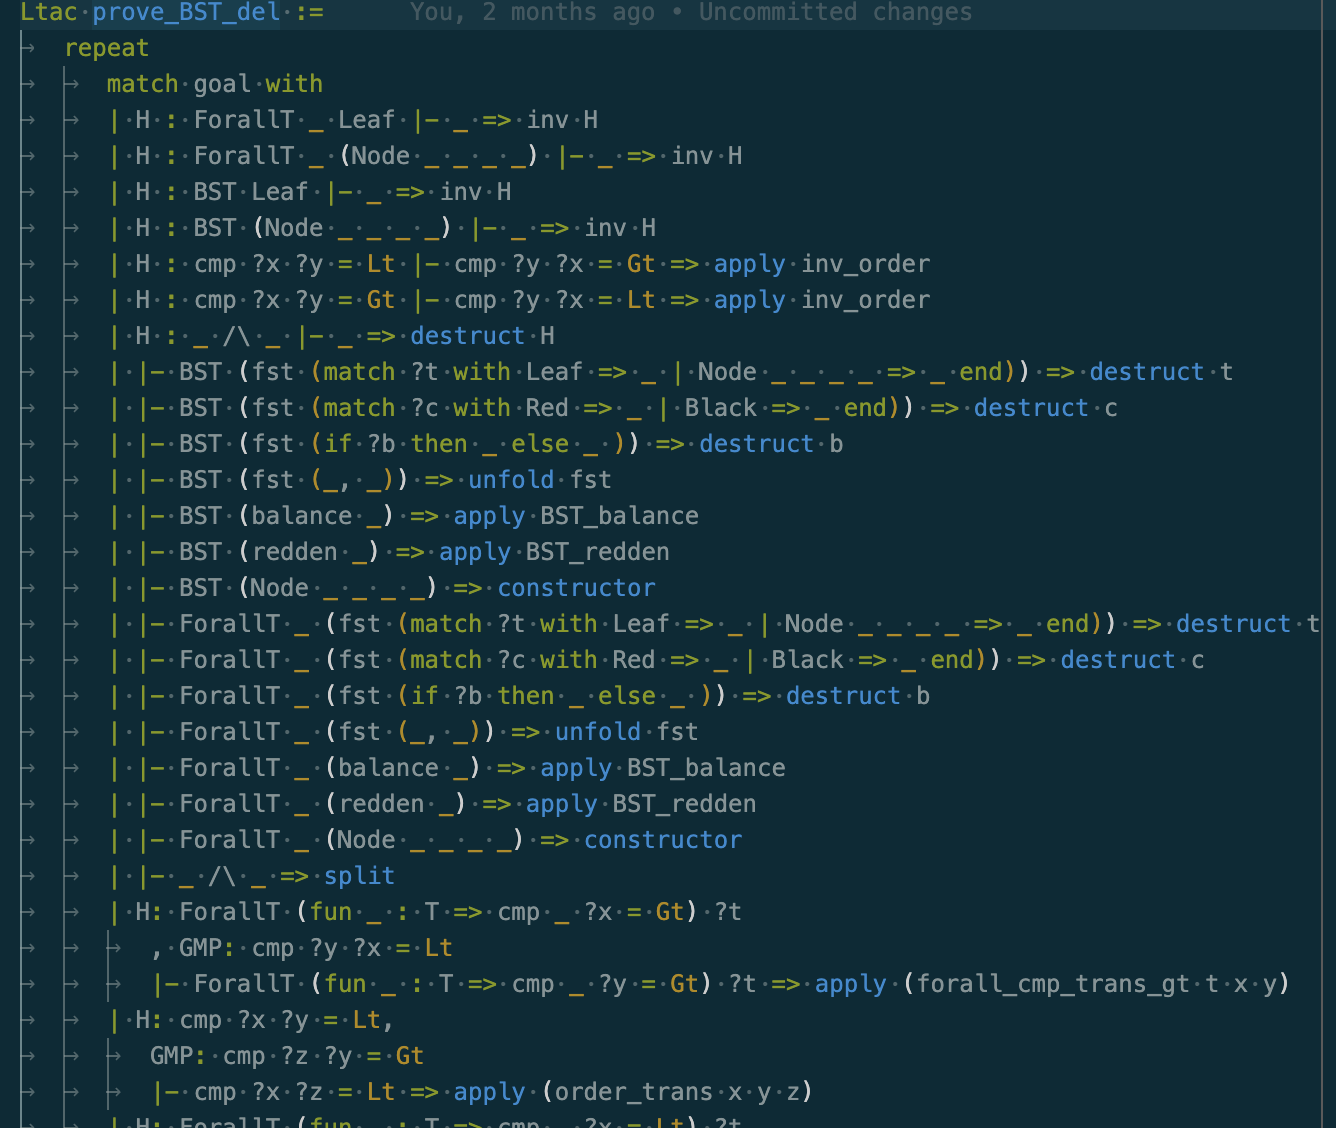
\includegraphics[width=0.7\textwidth]{pain/catch-all.png}
\end{frame}

\begin{frame}{Easy proof}
   \centering
   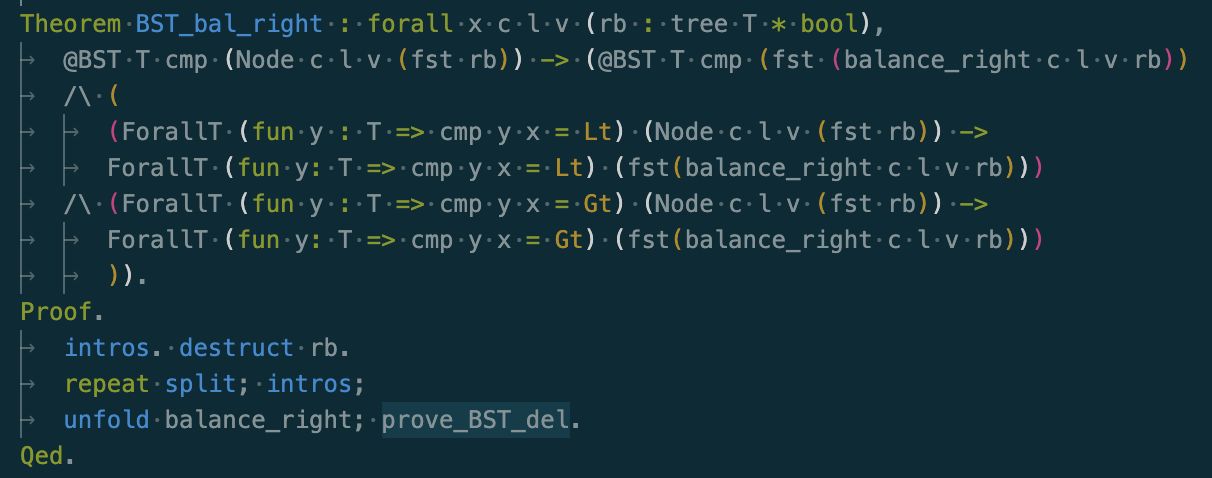
\includegraphics[width=0.7\textwidth]{pain/easy-proof.png}
\end{frame}

%-------------------
\begin{frame}{What I would like to see}
   \begin{itemize}
      \item Easy to find examples (Cookbook)
      \item High level libraries
      \item Definition vs Inductive vs Fixpoint vs ...
      \item Lemmas vs Theorem vs ...
      \item 'Easy refactoring tools'
   \end{itemize}
\end{frame}

%-------------------
\begin{frame}{Questions ?}
   \begin{center}
      \Huge Thank you !
   \end{center}
\end{frame}

\end{document}
